% Lines starting with a percent sign (%) are comments. LaTeX will 
% not process those lines. Similarly, everything after a percent 
% sign in a line is considered a comment. To produce a percent sign
% in the output, write \% (backslash followed by the percent sign). 
% ==================================================================
% Usage instructions:
% ------------------------------------------------------------------
% The file is heavily commented so that you know what the various
% commands do. Feel free to remove any comments you don't need from
% your own copy. When redistributing the example thesis file, please
% retain all the comments for the benefit of other thesis writers! 
% ==================================================================
% Compilation instructions: 
% ------------------------------------------------------------------
% Use pdflatex to compile! Input images are expected as PDF files.
% Example compilation:
% ------------------------------------------------------------------
% > pdflatex thesis-example.tex
% > bibtex thesis-example
% > pdflatex thesis-example.tex
% > pdflatex thesis-example.tex
% ------------------------------------------------------------------
% You need to run pdflatex multiple times so that all the cross-references
% are fixed. pdflatex will tell you if you need to re-run it (a warning
% will be issued)  
% ------------------------------------------------------------------
% Compilation has been tested to work in ukk.cs.hut.fi and kosh.hut.fi
% - if you have problems of missing .sty -files, then the local LaTeX
% environment does not have all the required packages installed.
% For example, when compiling in vipunen.hut.fi, you get an error that
% tikz.sty is missing - in this case you must either compile somewhere
% else, or you cannot use TikZ graphics in your thesis and must therefore
% remove or comment out the tikz package and all the tikz definitions. 
% ------------------------------------------------------------------

% General information
% ==================================================================
% Package documentation:
% 
% The comments often refer to package documentation. (Almost) all LaTeX
% packages have documentation accompanying them, so you can read the
% package documentation for further information. When a package 'xxx' is
% installed to your local LaTeX environment (the document compiles
% when you have \usepackage{xxx} and LaTeX does not complain), you can 
% find the documentation somewhere in the local LaTeX texmf directory
% hierarchy. In ukk.cs.hut.fi, this is /usr/texlive/2008/texmf-dist,
% and the documentation for the titlesec package (for example) can be 
% found at /usr/texlive/2008/texmf-dist/doc/latex/titlesec/titlesec.pdf.
% Most often the documentation is located as a PDF file in 
% /usr/texlive/2008/texmf-dist/doc/latex/xxx, where xxx is the package name; 
% however, documentation for TikZ is in
% /usr/texlive/2008/texmf-dist/doc/latex/generic/pgf/pgfmanual.pdf
% (this is because TikZ is a front-end for PGF, which is meant to be a 
% generic portable graphics format for LaTeX).
% You can try to look for the package manual using the ``find'' shell
% command in Linux machines; the find databases are up-to-date at least
% in ukk.cs.hut.fi. Just type ``find xxx'', where xxx is the package
% name, and you should find a documentation file.
% Note that in some packages, the documentation is in the DVI file
% format. In this case, you can copy the DVI file to your home directory,
% and convert it to PDF with the dvipdfm command (or you can read the
% DVI file directly with a DVI viewer).
% 
% If you can't find the documentation for a package, just try Googling
% for ``latex packagename''; most often you can get a direct link to the
% package manual in PDF format.
% ------------------------------------------------------------------


% Document class for the thesis is report
% ------------------------------------------------------------------
% You can change this but do so at your own risk - it may break other things.
% Note that the option pdftext is used for pdflatex; there is no
% pdflatex option. 
% ------------------------------------------------------------------
\documentclass[12pt,a4paper,oneside,pdftex]{report}

% The input files (tex files) are encoded with the latin-1 encoding 
% (ISO-8859-1 works). Change the latin1-option if you use UTF8 
% (at some point LaTeX did not work with UTF8, but I'm not sure
% what the current situation is) 
\usepackage[utf8]{inputenc}
% OT1 font encoding seems to work better than T1. Check the rendered
% PDF file to see if the fonts are encoded properly as vectors (instead
% of rendered bitmaps). You can do this by zooming very close to any letter 
% - if the letter is shown pixelated, you should change this setting 
% (try commenting out the entire line, for example).  
\usepackage[OT1]{fontenc}
% The babel package provides hyphenating instructions for LaTeX. Give
% the languages you wish to use in your thesis as options to the babel
% package (as shown below). You can remove any language you are not
% going to use.
% Examples of valid language codes: english (or USenglish), british, 
% finnish, swedish; and so on.
\usepackage[finnish,english]{babel}

\usepackage{adjustbox}

% Optional packages
% ------------------------------------------------------------------
% Select those packages that you need for your thesis. You may delete
% or comment the rest.

% Natbib allows you to select the format of the bibliography references.
% The first example uses numbered citations: 
\usepackage[square,sort&compress,numbers]{natbib}
% The second example uses author-year citations.
% If you use author-year citations, change the bibliography style (below); 
% acm style does not work with author-year citations.
% Also, you should use \citet (cite in text) when you wish to refer
% to the author directly (\citet{blaablaa} said blaa blaa), and 
% \citep when you wish to refer similarly than with numbered citations
% (It has been said that blaa blaa~\citep{blaablaa}).
% \usepackage[square]{natbib}

% The alltt package provides an all-teletype environment that acts
% like verbatim but you can use LaTeX commands in it. Uncomment if 
% you want to use this environment. 
% \usepackage{alltt}

% The eurosym package provides a euro symbol. Use with \euro{}
\usepackage{eurosym} 

% Verbatim provides a standard teletype environment that renderes
% the text exactly as written in the tex file. Useful for code
% snippets (although you can also use the listings package to get
% automatic code formatting). 
\usepackage{verbatim}

% The listing package provides automatic code formatting utilities
% so that you can copy-paste code examples and have them rendered
% nicely. See the package documentation for details.
% \usepackage{listings}

% The fancuvrb package provides fancier verbatim environments 
% (you can, for example, put borders around the verbatim text area
% and so on). See package for details.
% \usepackage{fancyvrb}

% Supertabular provides a tabular environment that can span multiple 
% pages. 
%\usepackage{supertabular}
% Longtable provides a tabular environment that can span multiple 
% pages. This is used in the example acronyms file. 
\usepackage{longtable}

% The fancyhdr package allows you to set your the page headers 
% manually, and allows you to add separator lines and so on. 
% Check the package documentation. 
% \usepackage{fancyhdr}

% Subfigure package allows you to use subfigures (i.e. many subfigures
% within one figure environment). These can have different labels and
% they are numbered automatically. Check the package documentation. 
\usepackage{subfigure}

% The titlesec package can be used to alter the look of the titles 
% of sections, chapters, and so on. This example uses the ``medium'' 
% package option which sets the titles to a medium size, making them
% a bit smaller than what is the default. You can fine-tune the 
% title fonts and sizes by using the package options. See the package
% documentation.
\usepackage[medium]{titlesec}

% The TikZ package allows you to create professional technical figures.
% The learning curve is quite steep, but it is definitely worth it if 
% you wish to have really good-looking technical figures. 
\usepackage{tikz}
% You also need to specify which TikZ libraries you use
\usetikzlibrary{positioning}
\usetikzlibrary{calc}
\usetikzlibrary{arrows}
\usetikzlibrary{decorations.pathmorphing,decorations.markings}
\usetikzlibrary{shapes}
\usetikzlibrary{patterns}


% The aalto-thesis package provides typesetting instructions for the
% standard master's thesis parts (abstracts, front page, and so on)
% Load this package second-to-last, just before the hyperref package.
% Options that you can use: 
%   mydraft - renders the thesis in draft mode. 
%             Do not use for the final version. 
%   doublenumbering - [optional] number the first pages of the thesis
%                     with roman numerals (i, ii, iii, ...); and start
%                     arabic numbering (1, 2, 3, ...) only on the 
%                     first page of the first chapter
%   twoinstructors  - changes the title of instructors to plural form
%   twosupervisors  - changes the title of supervisors to plural form
% \usepackage[mydraft,twosupervisors]{aalto-thesis}

\usepackage[twosupervisors]{aalto-thesis}
%\usepackage[mydraft,doublenumbering]{aalto-thesis}
%\usepackage{aalto-thesis}



% Hyperref
% ------------------------------------------------------------------
% Hyperref creates links from URLs, for references, and creates a
% TOC in the PDF file.
% This package must be the last one you include, because it has
% compatibility issues with many other packages and it fixes
% those issues when it is loaded.   
%\RequirePackage[pdftex]{hyperref}
\RequirePackage[pdfa]{hyperref}
% Setup hyperref so that links are clickable but do not look 
% different
\hypersetup{colorlinks=false,raiselinks=false,breaklinks=true}
\hypersetup{pdfborder={0 0 0}}
\hypersetup{bookmarksnumbered=true}
% The following line suggests the PDF reader that it should show the 
% first level of bookmarks opened in the hierarchical bookmark view. 
\hypersetup{bookmarksopen=true,bookmarksopenlevel=1}
% Hyperref can also set up the PDF metadata fields. These are
% set a bit later on, after the thesis setup.   


% Thesis setup
% ==================================================================
% Change these to fit your own thesis.
% \COMMAND always refers to the English version;
% \FCOMMAND refers to the Finnish version; and
% \SCOMMAND refers to the Swedish version.
% You may comment/remove those language variants that you do not use
% (but then you must not include the abstracts for that language)
% ------------------------------------------------------------------
% If you do not find the command for a text that is shown in the cover page or
% in the abstract texts, check the aalto-thesis.sty file and locate the text
% from there. 
% All the texts are configured in language-specific blocks (lots of commands
% that look like this: \renewcommand{\ATCITY}{Espoo}.
% You can just fix the texts there. Just remember to check all the language
% variants you use (they are all there in the same place). 
% ------------------------------------------------------------------
\newcommand{\TITLE}{Acoustic Information for\\Multisensory Occupancy Detection\\using Machine Learning}

% old title:  Machine Learning based Multisensory Room Occupancy Detection
% new: acoustic information for Embedded multisensory room occupancy detection using ml

\newcommand{\FTITLE}{Ohjelmistoprosessit mänteille:}
\newcommand{\STITLE}{Den stora stygga vargen:}
\newcommand{\SUBTITLE}{}
\newcommand{\FSUBTITLE}{Uusi organisaatio, uudet pyörät}
\newcommand{\SSUBTITLE}{Lilla Vargens universum}
\newcommand{\DATE}{\today}
\newcommand{\FDATE}{14. helmikuuta 2018}
\newcommand{\SDATE}{Den 18 februari 2018}

% Supervisors and instructors
% ------------------------------------------------------------------
% Usually thesis have one supervisor and one advisor. Sometimes you
% may have two advisors and, in double degree
% programs, you may have two supervisors. 
% If you have two supervisors, write both names here, separate them with a 
% double-backslash (see below for an example)
% Also remember to add the package option ``twosupervisors'' or
% ``twoinstructors'' to the aalto-thesis package (aalto-thesis.sty
% file line 72), so that the titles are in plural.
% Example of one supervisor:
%\newcommand{\SUPERVISOR}{Professor Tom Bäckström}
%\newcommand{\FSUPERVISOR}{Professori Antti Ylä-Jääski}
%\newcommand{\SSUPERVISOR}{Professor Antti Ylä-Jääski}
% Example of twosupervisors:
\newcommand{\SUPERVISOR}{Professor Tom Bäckström\\
 Professor Davide Brunelli}
%\newcommand{\FSUPERVISOR}{Professori Antti Ylä-Jääski\\
%  Professori Petra Perustieteilijä}
%\newcommand{\SSUPERVISOR}{Professor Antti Ylä-Jääski\\
%  Professor Petra Perustieteilijä}

% If you have only one instructor, just write one name here
\newcommand{\INSTRUCTOR}{Juha Kallas M.Sc. (Tech.)}
\newcommand{\FINSTRUCTOR}{Diplomi-insinööri Oili Ohjaaja}
\newcommand{\SINSTRUCTOR}{Diplomingenjör Oili Ohjaaja}
% If you have two instructors, separate them with \\ to create linefeeds
% \newcommand{\INSTRUCTOR}{Oili Ohjaaja M.Sc. (Tech.)\\
%  Elli Opas M.Sc. (Tech)}
%\newcommand{\FINSTRUCTOR}{Diplomi-insinööri Oili Ohjaaja\\
%  Diplomi-insinööri Elli Opas}
%\newcommand{\SINSTRUCTOR}{Diplomingenjör Oili Ohjaaja\\
%  Diplomingenjör Elli Opas}

% If you have two supervisors, it is common to write the schools
% of the supervisors in the cover page. If the following command is defined,
% then the supervisor names shown here are printed in the cover page. Otherwise,
% the supervisor names defined above are used.
\newcommand{\COVERSUPERVISOR}{Professor Tom Bäckström, Aalto University\\
Professor Davide Brunelli, University of Trento}

% The same option is for the instructors, if you have multiple instructors.
% \newcommand{\COVERINSTRUCTOR}{Oili Ohjaaja M.Sc. (Tech.), Aalto University\\
%  Elli Opas M.Sc. (Tech), Aalto SCI}


% Other stuff
% ------------------------------------------------------------------
\newcommand{\PROFESSORSHIP}{Autonomous Systems}
\newcommand{\FPROFESSORSHIP}{Tietotekniikka}
\newcommand{\SPROFESSORSHIP}{Datateknik}
% Professorship code is the same in all languages
\newcommand{\PROFCODE}{ELEC3055}
\newcommand{\KEYWORDS}{ Deep Neural Networks, Digital Signal Processing, Embedded AI, Lighting Control, MEMS Microphone, PIR, Presence Detection, Supervised Machine Learning }
\newcommand{\FKEYWORDS}{aineistot, aitta, akustiikka, Alankomaat,
aluerakentaminen, aapinen, ankka, aasinsilta}
\newcommand{\SKEYWORDS}{omsättning, kassaflöde, värdepappersmarknadslagen,
yrkesutövare, intresseföretag, verifieringskedja}
\newcommand{\LANGUAGE}{English}
\newcommand{\FLANGUAGE}{Englanti}
\newcommand{\SLANGUAGE}{Engelska}

% Author is the same for all languages
\newcommand{\AUTHOR}{Krist\'of Koszoru}


% Currently the English versions are used for the PDF file metadata
% Set the PDF title
\hypersetup{pdftitle={\TITLE\ \SUBTITLE}}
% Set the PDF author
\hypersetup{pdfauthor={\AUTHOR}}
% Set the PDF keywords
\hypersetup{pdfkeywords={\KEYWORDS}}
% Set the PDF subject
\hypersetup{pdfsubject={Master's Thesis}}


% Layout settings
% ------------------------------------------------------------------

% When you write in English, you should use the standard LaTeX 
% paragraph formatting: paragraphs are indented, and there is no 
% space between paragraphs.
% When writing in Finnish, we often use no indentation in the
% beginning of the paragraph, and there is some space between the 
% paragraphs. 

% If you write your thesis Finnish, uncomment these lines; if 
% you write in English, leave these lines commented! 
% \setlength{\parindent}{0pt}
% \setlength{\parskip}{1ex}

% Use this to control how much space there is between each line of text.
% 1 is normal (no extra space), 1.3 is about one-half more space, and
% 1.6 is about double line spacing.  
% \linespread{1} % This is the default
% \linespread{1.3}

% Bibliography style
% acm style gives you a basic reference style. It works only with numbered
% references.
\bibliographystyle{acm}
% Plainnat is a plain style that works with both numbered and name citations.
% \bibliographystyle{plainnat}


% Extra hyphenation settings
% ------------------------------------------------------------------
% You can list here all the files that are not hyphenated correctly.
% You can provide many \hyphenation commands and/or separate each word
% with a space inside a single command. Put hyphens in the places where
% a word can be hyphenated.
% Note that (by default) LaTeX will not hyphenate words that already
% have a hyphen in them (for example, if you write ``structure-modification 
% operation'', the word structure-modification will never be hyphenated).
% You need a special package to hyphenate those words.
\hyphenation{di-gi-taa-li-sta yksi-suun-tai-sta}



% The preamble ends here, and the document begins. 
% Place all formatting commands and such before this line.
% ------------------------------------------------------------------
\begin{document}
% This command adds a PDF bookmark to the cover page. You may leave
% it out if you don't like it...
\pdfbookmark[0]{Cover page}{bookmark.0.cover}
% This command is defined in aalto-thesis.sty. It controls the page 
% numbering based on whether the doublenumbering option is specified
\startcoverpage

% Cover page
% ------------------------------------------------------------------
% Options: finnish, english, and swedish
% These control in which language the cover-page information is shown
\coverpage{english}


% Abstracts
% ------------------------------------------------------------------
% Include an abstract in the language that the thesis is written in,
% and if your native language is Finnish or Swedish, one in that language.

% Abstract in English
% ------------------------------------------------------------------
\thesisabstract{english}{
% The abstract provides goal, motivation, background, and conclusions of the work. It has to fit to one page together with the bibliographical information.

% Goal
% - Creation of a multisensory room occupancy detection device for light automation using audio and motion sensors
% Motivation
% - 
% Background
% - 
% Conclusions
% - Introduction of audio information helped to reduce false negative predictions and allowed to operate with a shorter timeout value leading to more energy savings.

In this thesis, the combination of passive infrared (PIR) and audio sensors for indoor room occupancy detection was demonstrated, with a special focus on audio signal processing and feature extraction using Machine Learning techniques.
The lighting automation industry uses extensively PIR or motion sensors for presence detection due to their simplicity and low cost, but their small sensitivity for subtle movements makes them inefficient in certain situations. The occasional undesired behavior is often compensated with long timeout values but this leads to excessive energy consumption.


We are presenting a computationally efficient audio feature extraction method and using exhaustive grid search for Machine Learning model architecture optimization. The best-performing models provided the basis for the embedded implementation of a real-time occupancy device, which combines audio and PIR information for improved presence detection. The prototype performance was measured against the traditional PIR based solutions demonstrating lower false-negative predictions with shorter timeout values.
}

% Abstract in Finnish
% ------------------------------------------------------------------
%\thesisabstract{finnish}{
%Jos koulusivistyskielesi on suomi, diplomityössä pitää olla
%suomenkielinen tiivistelmä. Tiivistelmän pitää mahtua yhdelle
%
%Tiivistelmässä on yleensä useampia kappaleita. Tiivistelmä kertoo työn
%tavoitteet, motivaation, taustan ja johtopäätökset.
%}

% Abstract in Swedish
% ------------------------------------------------------------------
%\thesisabstract{swedish}{
%Om ditt skolespråk är svenska, måste din diplomarbetet  ha en svenskspråkig sammanfattning. %Sammanfattningen måste passa på en sida.}
%

% Acknowledgements
% ------------------------------------------------------------------
% Select the language you use in your acknowledgements
\selectlanguage{english}

% Uncomment this line if you wish acknoledgements to appear in the 
% table of contents
%\addcontentsline{toc}{chapter}{Acknowledgements}

% The star means that the chapter isn't numbered and does not 
% show up in the TOC
\chapter*{Acknowledgements}

Completion of this thesis would not have been possible without the help of several people. First of all, I would like to thank my supervisors, Tom Bäckström and Davide Brunelli for their guidance during the entire process of my graduation, and Juha Kallas and Henri Juslén for their valuable insights during the project development.

I would also like to extend my deepest gratitude to my family. To my dad, who has always found something around the house that needed to be repaired or built. I would have never become an engineer if I did not see the commitment and diligence on him. The same goes for my mom, who asked me every day what happened in school when I got home but allowed me to take risky hikes, and to study abroad.

% Finally, I am also grateful to the soldiers who allowed me to enter Italy and Finland at the border control in these uncertain times, and all the fellow students who showed up at my place during this two-year master's program in Trento and Espoo when I invited them for causal discussions.

Finally, I am also grateful to all the fellow students who showed up every time at my place during this two-year master's program in Trento or Espoo when I invited them to dinner or a simple gathering.



% Moreover I want to thank my father that after arriving home from work he never just lay back watching TV, but always kept pushing the tasks around the garden until dark. I would have never became an engineer without seeing the dedication on him. And most importantly I would like to express my gratitude towards my mother, who asked me every day what happened with me in school, and let me abroad to study.


% 
\vskip 10mm

\noindent Espoo, \DATE
\vskip 5mm
\noindent\AUTHOR

% Acronyms
% ------------------------------------------------------------------
% Use \cleardoublepage so that IF two-sided printing is used 
% (which is not often for masters theses), then the pages will still
% start correctly on the right-hand side.
\cleardoublepage
% Example acronyms are placed in a separate file, acronyms.tex
\addcontentsline{toc}{chapter}{Abbreviations and Acronyms}
\chapter*{Abbreviations and Acronyms}

% The longtable environment should break the table properly to multiple pages, 
% if needed

\noindent
\begin{longtable}{@{}p{0.25\textwidth}p{0.7\textwidth}@{}}
AI              &       Artificial Intelligence \\
ANN             &       Artificial Neural Network  \\
ASIC            &       Application-Specific Integrated Circuit      \\
ASR             &       Automatic Speech Recognition  \\
BN              &       Batch Normalization     \\
BSP             &       Board Support Package     \\
CMSIS           &       Cortex Microcontroller Software Interface Standard    \\
CNN             &       Convolutional Neural Network  \\
DCT             &       Discrete Cosine Transform  \\
DFT             &       Discrete Fourier Transform  \\
DMA             &       Direct Memory Access  \\
DSP             &       Digital Signal Processing  \\
ELU             &       Exponential Linear Unit  \\
ESC             &       Environmental Sound Classification  \\
FCN             &       Fully Connected Network  \\
FIR             &       Finite Impulse Response     \\
FLOP            &       Floating Point Operation   \\
FPU             &       Floating Point Unit  \\
GMM             &       Gaussian Mixture Model  \\
GPIO            &       General Purpose Input/Output    \\
HAL             &       Hardware Abstraction Layer     \\
HMM             &       Hidden Markov Model  \\
HVAC            &       Heating Ventilation and Air Conditioning   \\
I2S             &       Integrated Inter-IC Sound Bus  \\
IDE             &       Integrated Development Environment  \\
iHMM            &       infinite Hidden Markov Model   \\
IIR             &       Infinite Impulse Response     \\
IoT             &       Internet of Things  \\
ISR             &       Interrupt Service Routine     \\
LPCM            &       Linear Pulse Code Modulation   \\
LSB             &       Least Significant Bit     \\
MACC            &       Multiply And Accumulate      \\
MCU             &       Microcontroller Unit  \\
MEMS            &       Micro Electro Mechanical Systems   \\
MFCC            &       Mel-Frequency Cepstral Coefficients   \\
ML              &       Machine Learning \\
MLP             &       Multi-Layer Perceptron  \\
MSB             &       Most Significant Bit     \\
ONNX            &       Open Neural Network Exchange   \\
PCA             &       Principal Component Analysis  \\
PCM             &       Pulse Code Modulation  \\
PIR             &       Passive Infrared Sensor  \\
ReLU            &       Rectified Linear Unit   \\
RL              &       Reinforcement Learning \\
SPI             &       Serial Peripheral Interface     \\
SRAM            &       Static Random-Access Memory      \\
STE             &       Short-Time Energy  \\
SVM             &       Support Vector Machine  \\
UART            &       Universal Asynchronous Receiver-Transmitter   \\
UMAP            &       Uniform Manifold Approximation and Projection   \\
VAD             &       Voice Activity Detection  \\
ZCR             &       Zero Crossing Rate  \\
                &         \\
                &         \\



\end{longtable}


% Table of contents
% ------------------------------------------------------------------
\cleardoublepage
% This command adds a PDF bookmark that links to the contents.
% You can use \addcontentsline{} as well, but that also adds contents
% entry to the table of contents, which is kind of redundant.
% The text ``Contents'' is shown in the PDF bookmark. 
\pdfbookmark[0]{Contents}{bookmark.0.contents}
\tableofcontents

% List of tables
% ------------------------------------------------------------------
% You only need a list of tables for your thesis if you have very 
% many tables. If you do, uncomment the following two lines.
% \cleardoublepage
% \listoftables

% Table of figures
% ------------------------------------------------------------------
% You only need a list of figures for your thesis if you have very 
% many figures. If you do, uncomment the following two lines.
% \cleardoublepage
% \listoffigures

% The following label is used for counting the prelude pages
\label{pages-prelude}
\cleardoublepage

%%%%%%%%%%%%%%%%% The main content starts here %%%%%%%%%%%%%%%%%%%%%
% ------------------------------------------------------------------
% This command is defined in aalto-thesis.sty. It controls the page 
% numbering based on whether the doublenumbering option is specified
\startfirstchapter

% Add headings to pages (the chapter title is shown)
\pagestyle{headings}

% The contents of the thesis are separated to their own files.
% Edit the content in these files, rename them as necessary.
% ------------------------------------------------------------------
\chapter{Introduction}
\label{chapter:intro}
% 2-5 pages
%  It usually has two subsections with titles Problem
% statement and Structure of the Thesis, as follows next.


% Introduction tells the motivation, scope, goal and the outcome of the work. Anyone should be able to understand it. The preferred order of writing your master's thesis is about the same as the outline of the thesis: you first discover your problem and write about that, then you find out what methods you should use and write about that.  Then you do your implementation, and document that, and so on.  However, the abstract and introduction are often easiest to write last.  This is because these really cover the entire thesis, and there is no way you could know what to put in your abstract before you have actually done your implementation and evaluation. This means that you have to rewrite them in the end of your work.

% TOM COMMENTS:
%  - First paragraph is only one sentence, need a follow-up, for example highlighting that room-lighting uses a considerable amount of energy, which can be improved if lights were off when nobody is there.
%  - The intro overall is now nicely readable for people with an engineering background. I would recommend making this readable for an even wider range of people; My usual recommendation to use as a mental image, is that your parents should be able to understand this section. This applies primarily to the first page of the intro, the rest can be directed to people with an engineering background.

% Advanced level tuning of intro:

% 1. 
% Think about the overall structure, by labeling each paragraph, for example;
% - First paragraph "Energy consumption"
% - Second paragraph "Building automation"
% - Third "Occupancy detection"
% and so on. 

% Then make each paragraph balanced, in size and depth, with respect to the overall structure.

% 2.
% Finally, think about contrasts: An effective way to trigger reader interest is to alternate between good things and bad things, first slowly (long sections of only good and only bad), but then contrasting more and more frequently, until the climax where your fantastic solution to room occupancy detection wins the world. After the climax, the text is only about good things.

% If you manage to combine the two, balanced structure and increasing speed of contrasts, then that would elevate the literary quality from student work to a work of art.

% PETERRR
% too many "since" replace with as or for
% comma before too -> , too.

% Energy need increases
% Buildings use a lot of energy
In a world of rising energy needs and excessive usage of natural resources, the need for energy conservation has become ever more important lately. Global urbanization and population growth are clear trends of the twenty-first century. The proportion of people living in cities are increasing steadily. Residential and commercial buildings consume up to 40\% of world electricity \cite{perez2008_energyBuilding} according to IEA (International Energy Agency) statistics.

% Building automation
\begin{sloppypar}
Building Automation technologies have risen in popularity after the widespread use of large indoor offices and factories with the premise of cost reduction and later with increased comfort and well-being of workers. Simple control systems were used to regulate the properties of the building based on a predefined schedule only, which allowed only a limited amount of energy savings since they completely ignored the presence of people.
% https://www.zeroscience.mk/files/ioybms_gk_2019.pdf
\end{sloppypar}

% Occupancy measurements
Modern, flexible work arrangement policies raised new demand for more adaptive Building Management Systems to control building equipment that reacts quickly to space usage changes. Indoor room occupancy detection is an actively researched area, previous studies mostly focused on single sensor-based data analysis and future forecasting predictions to improve reliability and applicability to different scenarios. Most commonly used input data sources include passive infrared (PIR), Camera, Sound, Radar, CO\textsubscript{2}, and other Environmental sensors \cite{build_occ_det_tech_review}. Previous research has demonstrated the importance of occupancy data to reduce excess energy use \cite{ZHANG2018build_energy_occ, NGUYEN2013build_energy_occ}.
% https://journals.sagepub.com/doi/pdf/10.1177/1420326X19875621?casa_token=6d_4bFUbzTQAAAAA:xq__QTtH6Y5aHHFRAkTZ66BNJuSh65vo1PjxcRQSdaC1Io7lsssF9LpFxIluYbMs9xMxLD47IA
% 2 - A comprehensive review of approaches to building occupancy detection \cite{build_occ_det_tech_review}

% Sound information for occupancy, multisensor
Single sensor-based occupancy solutions carry the limitations of the chosen sensor inherently due to its physical properties. Some of them require a direct line of sight, sensitive to external noises, intrusive or non-intrusive in their operation. Research shows that the combination of various sensors can be beneficial for increasing prediction accuracy \cite{UCI_occ_dataset_pred, UCI_autoencoder, UCI_nn_real_time, Yang12multisensor_aud}. Our study will focus on the combination of PIR, as the most often deployed sensor in Building Automation, and sound sensors for enhancement.

% Solutions
% Machine learning and IoT
Machine Learning has been recently introduced to extract high-level information from sensor data streams. Classical machine learning and more advanced Deep Learning methods provide a universal platform for classification tasks given a large enough dataset for training. According to the traditional machine learning based Internet of Things (IoT) approach, the computationally heavy calculations are performed in a cloud service while the IoT devices only stream the raw sensor measurements.

%TODO: Internet of things, increasing trend in edge computation... \cite{wang2020fannonmcu}
% https://arxiv.org/pdf/1911.03314.pdf

% Cloud based solutions
However, the acceptance of cloud-based innovative Building Management solutions falls behind, due to privacy concerns and data bandwidth limitations mainly \cite{yu2016iot}. Moreover, from a user experience perspective, lighting automation solutions are expected to respond instantaneously to environmental changes or movements of people leaving no room for top-down cloud-based control with its inherent network latency.

% Embedded computation only
Mitigating the aforementioned limitations, the new trend is to allocate as much local data processing as possible creating the basis of smart sensor platforms or Edge Computing. According to this paradigm, the machine learning inference is pushed towards the edge of the network facilitating mostly on ARM-based microcontrollers. The research field related to embedded machine learning is relatively new, but some applications in production can already be spotted and expected to grow with the microcontroller hardware performance and software library support.

% My solution, goal of the thesis
This thesis aims to explore the possibilities of machine learning techniques in an embedded environment for occupancy detection in the current industrial setting. It provides a thorough analysis of the problem complexity and offers an effective real-time feature extraction and classification method for spotting human presence in sound and PIR sensor streams. 


\section{Problem statement}

The PIR (Passive Infrared) sensor is the most common device used for room occupancy detection in office environments, given its simple structure, low cost, and easy integration properties. It works satisfactorily mainly in motion detection tasks, where the big movement is a clear indicator of human activity such as in corridors.

The limitations of the technology arise when it is deployed to other kinds of office scenarios. Without any additional logic, it often fails to detect presence in meeting rooms given the detectable movement is usually very limited during a conversation.
This observation is usually compensated with long timeout values on the lighting control level, hoping that the sensor will pick up some movement in the given 15 or 30 minutes long window even in those situations. However, this approach leads to unnecessary extra energy consumption, since we have to wait at least 15 min for the light to turn off even if people left the meeting room, and discomfort due to false automatic behavior of luminaries.
Moreover providing true occupancy data could help optimizing space usage and lead to smarter and more environmentally friendly HVAC (Heating, Ventilation and Air Conditioning) control solutions, compared to the current PIR-based approximations.

The primary goal of the thesis is to explore novel approaches with the combination of sound and PIR sensors and machine learning techniques to improve the reliability of room occupancy detection and therefore reduce excess energy usage.


% In this last paragraph, which is now just a sentence, add a hypothesis or expectation of results, and why those results are important. Or describing the same thing in a different way. Always construct arguments such that they contain why, what and how. Now you explain only what you will do, a bit of how you will do it is there as well, but the why is missing. You did explain the why in the previous paragraphs, but it should be connected explicitly to the goal of this thesis.

\section{Structure of the Thesis}
\label{section:structure} 

%The structure of the thesis should help to present your merits: knowing the literature, understanding the theory, mastering the methods, and presenting the findings.

% example structure:
% 
% - Introduction (e.g. 5 pages)
% - Theory (10–15 pages)
% - Methods and materials (10–15 pages)
% - Analysis (15–20 pages)
% - Discussion (5–10 pages)
% - Conclusions (3–5 pages)


%You should use transition in your text, meaning that you should help the reader follow the thesis outline. Here, you tell what will be in each chapter of your thesis. Often the thesis does not have as many chapters as is in this template. For example, environment and implementation can be combined as well as chapters of evaluation and discussion.  The rest of this thesis is organized as follows. Chapter~\ref{chapter:background} gives the background, etc.


The Background chapter describes the recent findings of research areas closely related to the thesis topic such as Environmental Sound Classification, Voice Activity Detection, and Occupancy detection for indoor environments. Results of these papers support the understanding of the technologies used and the offered potential for the next advancements. After the general research overview, we will move to our specific case in Chapter 3 starting with the examination of input data used for machine learning purposes together with the theoretical explanation of key concepts in Digital Signal Processing needed to extract the most information possible. The next chapter starts with a high-level overview of currently popular machine learning tools with the focus of Deep learning model structures which are needed in the search for the best model for our purpose. The training procedure, effect of different model sizes, and prediction accuracy comparison will be presented. After experimenting with different model structures and hyper-parameter settings Chapter 5 offers a real-time embedded hardware implementation of the trained model with the sensors needed for data collection, while in the following chapter the test results of the deployed model are discussed with various performance measures. Finally, the thesis ends with the Conclusion part summarising shortly the research findings and offers promising ideas for future advancements of the project.




%Chapter & Content
%Background & Literature review
%Environment &  Data used for ML
%Methods &  ML models, comparison
%Implementation & Model deployment to EDGE
%Evaluation &  Test of the EDGE-AI, compare to ground-truth
%Discussion  &
%Conclusions   &













\chapter{Background}
\label{chapter:background} 

% \emph{[Literature review: ESC findings - Enviromental Sound Classification (also embedded implementations), VAD findings - Voice Activity Detection, PIR room occupancy research, keyword spotting, Edge AI?]}
% \bigskip

% Probably you should change the title to something that describes more the content of this chapter. Background consists of information that help other masters of the same degree program to understand the rest of the thesis. Often the background has two parts: the first part tells the theoretical background and the second one describes the background tied to the implementation.


% LAURAA
% too long etc..
% In Chapter 2, you should try to fit the intro to the chapter (before 2.1 begins) in one paragraph.  In my opinion, it is not necessary to discuss the contents of subsubchapters (2.1.x) in the opening.  
% Contents of 3.1.1. would perhaps fit better in 2.1 because now you discuss PIR problems before telling much about what PIR is and how it works. 

%the three main topics
% - Acoustic Scene Classification
% - Room occupancy 
% - Edge-AI
 
This chapter provides a general introduction to research areas and insights closely related to the thesis topic.
%Moving on, the remaining part of the chapter presents the latest scientific achievements and industrial best practises in presence detection and information extraction from audio.
The Acoustic Scene Classification section will give a general overview of the latest research publications and most common industrial approaches dedicated to high-level information extraction from audio.

After the general introduction to the strictly sound-related research,we are going to narrow our focus to Room Occupancy research outcomes, detecting or counting people in indoor environments. Providing an overview on the various sensors researchers historically tested in different scenarios and their usability in several situations.

%More importantly with a special focus on Environmental Sound Classification and Voice Activity Detection research fields, which are the closest to the problem description of the thesis. These well-established fields had a great impact on the applied technologies and their well organized datasets and ready made solutions provided a clear guidance in the development of the audio processing part of the project. 

Some of the papers describe the implementation and test results of the developed algorithms on embedded platforms too, which helps to position the problem in the computational complexity and feasibility space. The increased computational requirement for novel deep learning model inference on edge devices often imposes a hard limit for real-time usability.


Finally, a short overview of Edge-AI will close the chapter, since in most cases the incentive is to run the advanced machine learning algorithms exclusively on embedded level. Given that it is an early stage but rapidly evolving field, the aim is to provide an overall picture of the capabilities and hard limitations using this approach.




\section{Acoustic Scene Classification}

Extracting high-level information from a given audio flow is a well-researched area with recent breakthroughs in many fields including Automatic Speech Recognition (ASR) to convert the live speech to text, Speaker Recognition, or Speech Separation using end-to-end Deep learning. Human presence can be associated with many different types of noises in indoor office environments. Speech is the most obvious one but even silent work with computers involves noises like typing, footsteps, breathing, and many others which might also reveal room occupancy. Among the mentioned alternatives, detection of speech will be the focus of the thesis, given it is the easiest and loudest signal for a human listener to differentiate between an occupied and an unoccupied meeting room. Moreover, speech frequencies and tones are characteristic of people while squeaking noises can be generated by other sources outside the examined area leading to false predictions.

In the next sections, we will exclusively concentrate on research fields where the goal is to spot human voice regardless of the content of the speech. The problem definition is simpler than for most recognition tasks, but could be sufficient for the scope of the thesis, where the meaning of the speech is considered to be irrelevant.

% Consider if you want to explain why and how detecting speech was selected. The "ultimate goal" would be spot "all" voices created by human presence (like typing, steps, chair noise or even breathing) but spotting pure speech was chosen to be in the scope of the thesis.

\subsection{Environmental Sound Classification (ESC)}
The goal of ESC is to classify audio recordings with a given length into one of the predefined classes which best describes the environment it was recorded in. The ESC-50 dataset \cite{ESC_dataset} is a labeled collection of audio samples for 50 categories, ranging from various animal, human and natural soundscapes to urban noises.A subset of the collection will be beneficial for training our DNN models in a different context and some of the research findings can also be translated into our domain.

\subsection{Voice Activity Detection (VAD)}
The Voice Activity Detector can be often found as one of the first modules in Automatic Speech Recognition (ASR) algorithms. Its only function is to detect at the lowest cost whether the audio stream contains speech or not, which needs to be further processed by more resource-intensive functions.

Approaches involve Gaussian Mixture Models (GMM) \cite{reynolds2009gaussianMM} and Hidden Markov Models (HMM) \cite{eddy2004hiddenMM}, like in the WebRTC VAD \cite{webrtc_vad}, developed by Google for real-time communication through the internet. Although their relatively simple architecture made it possible to run constantly in the background with low computational cost, they often face difficulties to spot speech in noisy environments. To overcome this issue modern VADs usually apply deep neural network models after feature extraction in the frequency domain. Test results are suggesting that both feed-forward and recurrent neural network structures can produce accurate predictions for the task \cite{sehgal18convolutional_vad}, although computationally heavy networks can be impractical for real-time embedded inference, regardless of their high accuracy.

% VAD sources:
% https://github.com/nicklashansen/voice-activity-detection
% https://github.com/nicklashansen/voice-activity-detection/blob/master/vad.ipynb
% https://github.com/hcmlab/vadnet

% WebRTC VAD
% https://webrtc.github.io/samples/
% https://developer.mozilla.org/en-US/docs/Web/API/WebRTC_API

The QUT-NOISE \cite{qut_noise} background noise, and the TIMIT \cite{timit} clean speech corpus serve as the base for constructing the QUT-NOISE-TIMIT dataset as well known training dataset and benchmark for VAD algorithms. Following the provided procedure over 600 hours of audio can be generated by mixing the noise and speech files with various target signal-to-noise ratios (SNR).

\section{Room occupancy detection research}

%input
Earlier research tackles the presence detection problem using a wide variety of sensors ranging from the conventional PIR, CO2, camera, sound, and environmental sensors to alternative, indirect approaches, mostly based on network activity and electricity usage. Cameras are generally used in this context only to establish only the ground truth for learning-based methods for other types of sensors, due to their high intrusiveness. \autoref{tab:comp_sensor} provides an overview of the most recent sensor technologies in research and their current capabilities. 

%sensor alternatives literature overview
% \cite{build_occ_det_tech_review}, algorithms
% \cite{build_occ_det_tech_review_sensor} - sensors

\begin{table}[]
\centering
\begin{adjustbox}{max width=0.95\textwidth}
\begin{tabular}{lllll}
\hline
\textbf{Sensor type}           & \textbf{Intrusiveness} & \textbf{Cost} & \textbf{Level of occupancy}                  & \textbf{References} \\ \hline
PIR                            & Low           & Low  & Presence, location                   & \cite{Naray15PIR_loc, PIR_only_behav_ext,PIR_only_behav_ext_mcu,PIR_tracking_yang2019new}          \\
CO\textsubscript{2}                            & Low           & Low  & Presence, location, count, activity  &  \cite{Yang12multisensor_aud,Newsh10PIR_CO2, CALI2015co2_anal}          \\
Camera                         & High          & High & Presence, location, count, activity, &  \cite{SHIH2014camera}          \\
                               &               &      & \hspace{0.5cm}tracking, identity     &            \\
Ultrasonic                     & Low           & Low  & Presence, location                   &  \cite{Shih16ultrason}           \\
Sound                          & Medium        & Low  & Presence, location                   & 
\cite{Aud_crowd_entropy_Chen, Aud_crowd_ste_huang, aud_gm_hmm, Yang12multisensor_aud}           \\
Environmental                  & Low           & Low  & Presence                             &   \cite{Yang12multisensor_aud}         \\
Tag based (Alt.)               & Low           & Low  & Presence, count, identity, location  &  \cite{Li16rfid_occ}           \\
Smart device based (Alt.)      & High          & High & Presence, location, count, activity, &   \cite{Gupta13WIFI_occ}         \\
                               &               &      & \hspace{0.5cm}tracking, identity     &            \\
Network activity based (Alt.)  & High          & Low  & Presence, count, location, identity  &   \cite{Newsh10PIR_CO2}         \\
                               &               &      & \hspace{0.5cm}activity               &            \\
Electricity usage based (Alt.) & Low           & High & Presence, location, activity         &   \cite{Newsh10PIR_CO2}           \\ \hline
\end{tabular}
\end{adjustbox}
\caption{Comparison of sensing approaches in occupancy detection research, adapted from \cite{build_occ_det_tech_review_sensor}.}
\label{tab:comp_sensor}
\end{table}



%alg
\begin{sloppypar}
Rueda et al. \cite{build_occ_det_tech_review} grouped the occupancy detection algorithms into three main categories in their literature review: analytical, data-driven, and knowledge-based. Analytical techniques aim to construct a mathematical relationship between the occupancy state and the measured sensor values. Cali et al. \cite{CALI2015co2_anal} developed a dynamic model for approximating the number of occupants by the measured CO\textsubscript{2} concentration in the room and predicted correctly 80.6\% of the time in their test environments.
\end{sloppypar}

Data-driven solutions often involved various modeling tools such as infinite hidden Markov model (iHMM) \cite{rasmussen1999infiniteGM}, hidden Markov model (HMM), k-means clustering \cite{hartigan1979kmeansclus, likas2003globalkmeansclus}, Support Vector Machines (SVM) \cite{noble2006supportVM}, Bayesian inference, and artificial neural network approaches \cite{Yang12multisensor_aud, UCI_nn_real_time}. Agarwal et al. \cite{rajesh10occ_rules} designed a knowledge-based system with magnetic door sensors and PIR sensor modules and managed to detect occupancy correctly with the predefined rules for expected system behavior.

%output
Occupancy detection systems can be divided into two general categories related to their measurement output. Simpler presence detectors can only indicate human presence as binary information (0 or 1), while more complex systems are able to classify the number of people, their location, identity, current activity, or even the direction of motion in the examined area, depending on the applied sensors and data processing approaches.



\subsection{PIR only}
It has been a growing effort to extract occupancy count, movement direction, human position, and behavioral features based on the analog output of a single or multiple PIR sensors arranged in a predefined way across the given space. 

Raykov et al. \cite{PIR_only_behav_ext} demonstrated that occupancy count can be extracted with $\pm$ 1 individual accuracy even from a single analog PIR sensor output by modeling the PIR output with Laplace distributions and clustering it with infinite hidden Markov model (iHMM) to group similar patterns. The approach worked best in cases of less than 8 people with a relatively long, 20 minutes applied time window.
% https://publications.aston.ac.uk/id/eprint/29352/1/Predicting_room_occupancy_with_a_PIR_sensor_through_behavior_extraction.pdf
They also provide a real-time microcontroller-based solution \cite{PIR_only_behav_ext_mcu} achieving more than 80\% accuracy on 1500 samples for a 30 seconds window while consuming less than 50 mW.
% https://www.researchgate.net/publication/314151438_Real-time_Room_Occupancy_Estimation_with_Bayesian_Machine_Learning_using_a_Single_PIR_Sensor_and_Microcontroller

Yang et al. \cite{PIR_tracking_yang2019new} used the analog PIR data from multiple sensors to estimate the azimuth angle of a moving person and with multiple sensor predictions localize it in a predefined area. The average localization error was strictly decreasing as they added more sensors to the experiment and reached as low as 0.63m with 4 sensors applied. Narayana et al. \cite{Naray15PIR_loc} built an array of PIR sensors and also with analog signal processing techniques managed to classify moving objects and localize them with 30 cm accuracy with 80 \% confidence in 5 m range.
% https://arxiv.org/pdf/1901.10700.pdf


\subsection{Sound only}
Solely microphone-based research in this domain mainly aims to estimate crowd size by extracting various features from the audio signal. One naive approach assumes that all the participants are speaking relatively at the same time and in this case the energy of the recorded signal will be proportional with the number of people. While more advanced solutions compute the Mel-Frequency features to better distinguish speech from general noise produced by non-human sources.

Huang et al. \cite{Aud_crowd_ste_huang} proposed a crowd size estimation technique based on Short-Time Energy (STE) computed on a 50 ms window, and tested it in a simulated environment using the TIMIT speech dataset \cite{timit} modeling the size of the room and the relative position of people to the microphone. The simulation only used clear recordings of people and did not take the room acoustics into account. For increased robustness, they fit a probability density function of data collected for 5 or 20 seconds and classify with respect to the maximal value and the theoretically established baseline derived from the simulation parameters. While in the following paper Huang  \cite{Aud_sound_cancellation} lays down an approach for noisy environments using background noise cancellation before the STE computation which leads to an 11\% increase in average detection accuracy.
% https://core.ac.uk/download/pdf/60582955.pdf
% https://www.mdpi.com/2075-5309/8/6/78?type=check_update&version=1
Chen et al. \cite{Aud_crowd_entropy_Chen} proposed an entropy-based method for the same problem.
% https://www.isca-speech.org/archive/Interspeech_2017/pdfs/0070.PDF

Valle in \cite{aud_gm_hmm} developed algorithms based on their audio dataset collected in a retail shop with a smartphone and labeled with the help of Amazon's Mechanical Turk. For the people counting prediction, the Mel-Frequency Cepstral Coefficients (MFCC) and their first and second deltas turned to be the most useful in their analysis. Given a total of 60 features (20+20+20) as an input to the Gaussian Mixtures and Hidden Markov Model (GM-HMM) the algorithm was able to predict occupancy up to 200 people reasonably accurately.
% https://www.researchgate.net/publication/305655038_ABROA_Audio-Based_Room-Occupancy_Analysis_using_Gaussian_Mixtures_and_Hidden_Markov_Models


\subsection{Multisensor based}
\label{section:Multisensor_research}
More recent research uses multiple environmental sensor sources for the hope of increased reliability and robustness in occupancy prediction. Even if the new sensor measurements such as light level or temperature would not be sufficient for presence detection on their own, but they can contribute new features for the final prediction model.

Candanedo et al. \cite{UCI_occ_dataset_pred} collected temperature, relative humidity, light, CO\textsubscript{2} levels and computed a humidity ratio in a test office room while a camera recorded the true occupancy for model fitting purposes. They have published the data set freely available on the UCI University domain. Their methods involved Linear Discriminant Analysis (LDA), Classification and Regression Trees (CART), and Random Forests (RF) reaching 95\%$+$ accuracy in their environment. However, since the lights were manually operated during the experiment it features an overwhelmingly high correlation with the occupancy, but with a false sense of confidence. The final models could not be used in different environments or controlling the lights based on occupancy, like in our case, since nobody would give this reliable input with a manual light switch.
% https://www.researchgate.net/publication/285627413_Accurate_occupancy_detection_of_an_office_room_from_light_temperature_humidity_and_CO2_measurements_using_statistical_learning_models
% nice comparison of previous approaches

There have been various developments on the same data set introducing deep learning methods for performance improvements. Liu et al. \cite{UCI_autoencoder}  first trained a sparse Auto-encoder structure for feature extraction before the Support Vector Machine (SVM) and Liblinear classifiers, while simple Feed-forward Neural Networks were used in \cite{UCI_nn_real_time}.
% https://ieeexplore.ieee.org/document/7912203



\section{EDGE-AI}
The constant improvements of embedded hardware performance and efficiency have opened the door for a new era of computing in machine learning, which focuses on local data processing for inference, eliminating the need for cloud computation and data streaming. Although current Edge AI solutions \cite{chen2019deep_edge_review} still rely on external computation for speeding up the training process, the prediction steps can be computed on the device exclusively. Taking this approach often yields better response time than the cloud-based counterpart, due to the elimination of network and additional latency \cite{zhou2018robust_edge_ai}. Edge AI offers an elegant solution for privacy concerns too since the sensitive information does not need to leave the device, can be processed locally, and therefore devices can be designed without any network connection.

The limited processing power of microcontrollers restricts the maximal size, type, depth of artificial neural networks by a significant amount. Techniques like quantization and network pruning of trained models can reduce the computational complexity in systems without floating-point arithmetic while maintaining prediction accuracy \cite{han2016deep_quant_prun}.
%The emergence of Edge AI and the rapid improvements in hardware development opened the door for ideas which could not been possible to implement before due to computation or network constraints. 
Chip manufacturers are fueling the innovation with alternatives on low power system-on-a-chip (SoC) devices, mostly developing dedicated hardware accelerators for AI inference purposes. This initiative can manifest in various forms with increased memory and bandwidth for Deep Learning model weights and dedicated matrix multipliers for a reduced delay in forward-pass.

High-performance yet affordable embedded platforms and tools motivated this work to explore the feasibility and applicability of the combination of machine learning and embedded audio processing in the presence detection space.


\chapter{Environment}
\label{chapter:environment}

% Most often you need to describe the environment you work in, what limits there are and so on. This is a good place to do that. Sometimes the environment is described together with your own implementation, in the same chapter.

% \emph{[ - Data and data preprocessing - , Audio, PIR, time/frequency domain, Mel-Frequency spectrum, MFCC, Data collection circumstances, Ground truth with camera]}
% \bigskip

In this chapter, we will give an overview of the basics of audio and PIR signal processing needed to understand the practical implementation of the multisensory prediction model. Since the goal is to classify different events, in the preprocessing step we aim to generate the most insightful but minimal set of features, from which presence can be easily detected. Our research will include time and frequency domain analysis of the audio signal and a basic introduction of the PIR sensor data.



\section{Raw PIR data processing}

Passive Infrared (PIR) sensors are the most widely used devices for motion detection and presence estimation for indoor spaces. Due to its simplicity, one sensor is incapable of distinguishing the source of movement or its direction. However, more options are available using analog sensors, since the sensitivity can be adjusted on the field for different applications and more information can be extracted from the signal waveform.

\subsection{The PIR sensor}
% TODO: better PIR sensor description Michrophonics: occupancy sensor technologies white paper pdf
 %PIR sensors are the most widely used devices for motion detection and presence estimation for indoor spaces. 
 The PIR sensor exploiting the pyroelectric properties of the applied materials, it can convert the absorbed infrared radiation into measurable analog voltage after a signal amplification step. 
 To be able to detect movement in the sensor field of view, PIR sensors split at least two parts and measure the relative difference between them canceling out the absolute radiation always present in the room. Additionally, focusing the IR rays to the different sensor elements, a custom-designed Fresnel lens is used, precisely controlling detection area and sensitivity. An example of a typical detection area arrangement for a ceiling-mounted PIR sensor can be seen in figure \ref{fig:pir_fov}. Sensor manufacturers are offering a wide variety of lenses tailor-made for the most common use cases ranging from horizontally wide detection areas for corridors to long-distance detection for sports halls with 7-10 meters expected installation height.

\begin{figure}[ht!]
  \begin{center}
    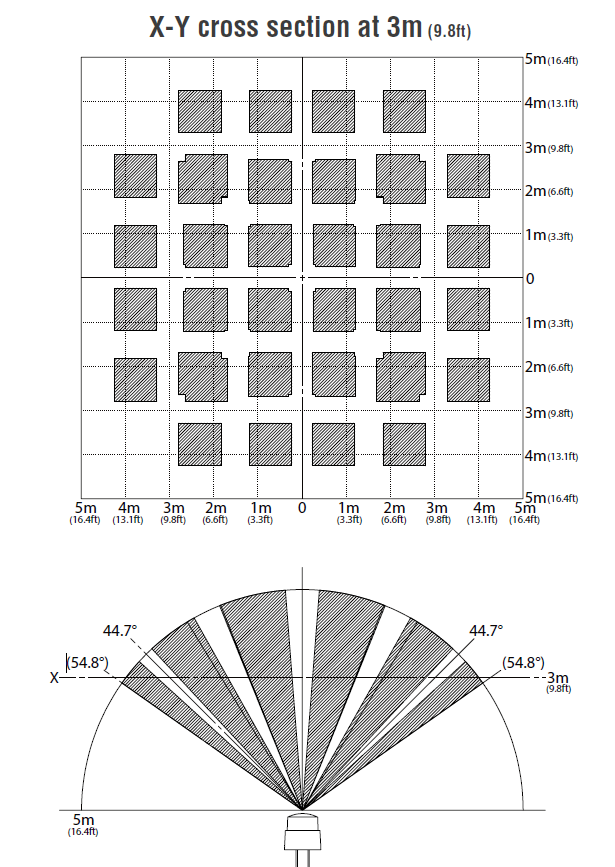
\includegraphics[width=0.5\textwidth]{thesistemplate/fig/pir_fov.png}
    \caption{Field of view of an industrial PIR sensor \cite{papir_dsheet}, the arrangement and sizes of detection zones are controlled by custom lens design.}
    \label{fig:pir_fov}
  \end{center}
\end{figure}

PIR sensors detect humans by their body temperature relative to the surrounding environment. As the thermal radiation for people mostly consists of infrared waves, it is sufficient to construct a sensor exclusively dedicated to spotting the IR level change in its switching zones. Sensor sensitivity can be increased by careful design of the lens, dividing the detection area into multiple smaller switching zones. Detection sensitivity is up to 4 \textdegree C at sensor level in most cases, between the background and the target object.


% JUHAA
%  You could also mention, that digital PIR variants often have integrated electronics providing output hold time (from seconds to minutes, configurable by user). This enables direct lighting control output.
From an application point of view, there are many variations of PIR sensors are available on the market. Starting from the most simple solution, analog PIR sensors provide direct access to the sensing elements with or without signal conditioning by an additional Amplifier circuit. To provide digital output, manufacturers integrate a Comparator circuit too after the signal amplification with a fixed threshold to distinguish between motion and steady-state. Moreover, the most complex digital PIR products offer adjustable sensitivity and output hold time with potentiometers. This way the signal output can be kept high for seconds or even minutes, which makes them applicable for direct lighting control without additional electronics.


Due to their physical properties, PIR sensors require a direct line of sight, which makes them hard to use in some special circumstances where people can be occluded by partitions or larger machines. Extensive deployment of single PIR sensors might mitigate the problem, but for a robust and flexible solution companies tend to deploy new approaches for more reliable presence detection.

%https://b2b-api.panasonic.eu/file_stream/pids/fileversion/4540
%https://na.industrial.panasonic.com/products/sensors/sensors-automotive-industrial-applications/lineup/pir-motion-sensor-papirs




\section{PIR based occupancy detection issues}

PIR or movement detection sensors are essential building blocks of automated lighting control systems. Unfortunately movement only is sometimes not sufficient to detect human presence, given the fact that PIR sensors are often not as sensitive to catch small changes in posture or breathing, therefore to avoid incorrectly turning the light off, they apply relatively long timeout values. 

Increasing the waiting time for new detected movement will improve system stability, but it also increases excess energy usage inevitably. By adjusting this interval the system can be tuned manually but due to the unpredictable nature of human activities, it falls far short of optimal behavior. Moreover, based on experience, PIR sensors can also produce false-positive triggers occasionally, due to various effects. Sudden changes in temperature, electromagnetic noises, or other building automation systems such as automatic window opening and curtain movements can trigger the sensor and lead to false lighting control scenarios. 


\begin{figure}[ht!]
  \begin{center}
    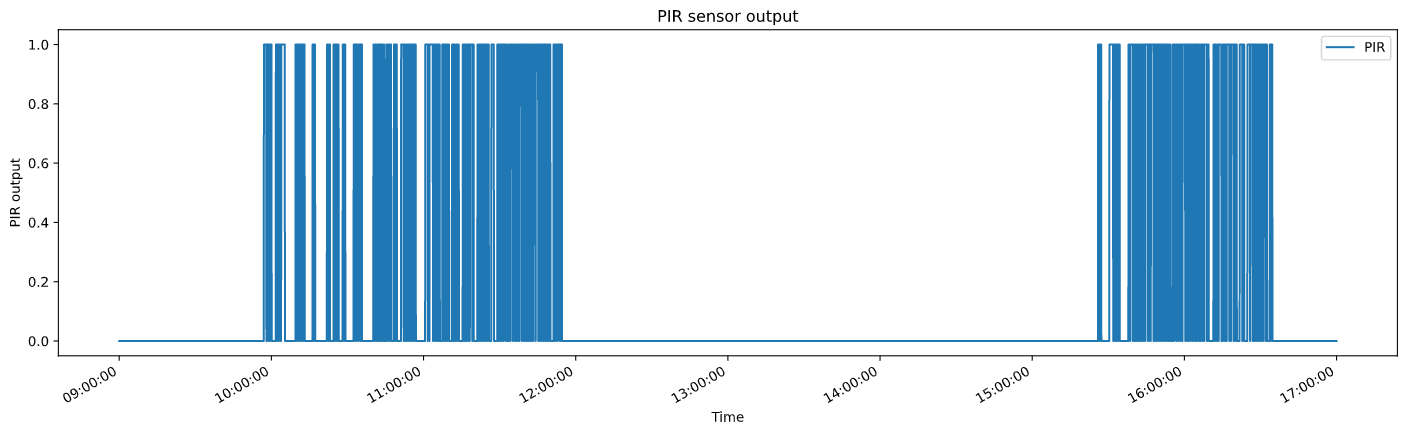
\includegraphics[width=1\textwidth]{thesistemplate/fig/pir_sensor_output.png}
    \caption{Raw output from a ceiling mounted PIR sensor during a working day, high output corresponds to detected movement.}
    \label{fig:state_mach}
  \end{center}
\end{figure}

% \subsection{PIR sensor output}

% Here we could display the difference between an analog and a digital PIR sensor output with a graph. The digital version mostly just a simplified version of the analog employing an amplifier and a comparator with a static threshold.

\section{Audio signal processing}

Audio signal processing is an engineering discipline concerned with the analog or digital manipulation of audio signals. To help to understand the implementation part of the thesis we only cover the most important concepts essential for comprehension.

\subsection{Audio signal}

After vision, the second most important sense humans rely on for information gathering from our closest environment is hearing. A sound signal is defined as sound pressure change over time, which propagates through a transmission medium. The generally accepted audio frequency range is 20 Hz to 20 kHz \cite{rosen2011signals_speech}, but studies show that the hearing sensitivity declines, especially in the upper-frequency range starting from early adulthood \cite{jilek2014hearing_loss}. 

Considering human sound-producing capabilities the organ larynx plays the most important role, and more strictly the vocal folds inside it \cite{rossing02the_science_of_sound}. The mass and length of vocal folds determine the typical or fundamental frequencies used in speech, which varies slightly between the sexes. Males use lower frequencies in general with a fundamental frequency around 110~Hz compare to 220~Hz with females and 300 Hz with children, but there is a high variance amongst individuals. \cite{rossing02the_science_of_sound} 

%JUHAA
% The Science of Sound. Rossing, Moore Wheeler, 3rd edition.
% Speech production, Chapter 15, Page 339:

% "The rate of vibration of the vocal folds is determined primarily by their mass and tension, although the pressure and velocity of the air do contribute in a smaller way. The vocal folds are typically longer and heavier in the adult male than in the female and, therefore, vibrate at a lower frequency (pitch). During normal speech, the vibration rate may vary over a 2:1 ratio (one octave), although the range of a singer's voice is more than two octaves. Typical frequencies used in speech are 110 Hz in the male, 220 Hz in the female and 300 Hz in the child, with wide variations from one individual to another."

The microphone is the most commonly used device to convert the sound pressure change into an electrical signal, firstly to a continuous analog signal then through sampling and discretization to digital audio. This step is inevitable in situations, where any kind of digital filtering or postprocessing is required for signal enhancement or manipulation.


\begin{figure}[ht!]
  \begin{center}
    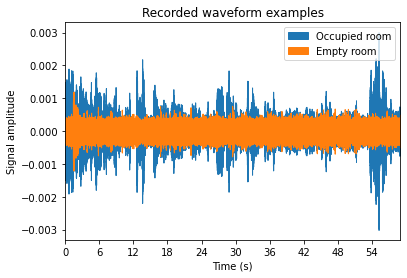
\includegraphics[width=0.6\textwidth]{thesistemplate/fig/recorded_waveform_ex.png}
    \caption{One minute normalized audio signal from empty and occupied room scenarios.}
    \label{fig:raw_aud_plot}
  \end{center}
\end{figure}


\subsection{Pulse Code Modulation}

Pulse code modulation (PCM) refers to a coding method used to transform analog waveforms to digital signals by sampling in time domain and quantization in value. Sampling frequency or sample rate determines the number of samples in one second, which reduces the continuous-time signal to a sequence of discrete values at specified time intervals. The selected sampling rate will affect the maximal bandwidth of the signal which can be reconstructed correctly without aliasing effects. According to the Nyquist Sampling Theorem, a continuous-time signal can be accurately reconstructed from its samples if the sampling frequency is at least twice as large as the highest frequency component.

\begin{equation*}
    f_{max} < f_s / 2
\end{equation*}

So choosing a sampling rate $f_s$ of 8 kHz will limit the signal to frequencies between 0 and 4 kHz. If the signal contains higher frequency components it needs to be filtered out by a low-pass filter to avoid aliasing effects.
%JUHAA
% Mention here Nyquist rate. Fs/2 gives upper limit of the signal frequency range. So 8kHz Fs means that signal can include frequencies in between 0 - 4kHz. If analog signal includes higher frequencies before AD, signals at higher frequencies will fold to lower frequencies. This is why signal should be always low-pass filtered before AD. MEMS mic with I2S output takes care of that for you.
The most commonly used sampling rates are 8000 Hz in telecommunication, 44,100 Hz as the standard CD quality, or 48000 Hz as audio channels for movies.


Although in some professional use cases might require an even higher sample rate in special circumstances. While in value, bit depth and the quantization levels  have to be defined. PCM as a general term is often used to describe LPCM or Linear pulse code modulation coding as the most commonly used  quantization method. LPCM features uniformly distributed levels for digitization purposes and the number of possible discrete values determined by the bit depth. The CD standard uses 16-bit resolution while modern digital media services apply 20, 24-bit depth for a bigger dynamic range representation.


\begin{figure}[ht!]
  \begin{center}
    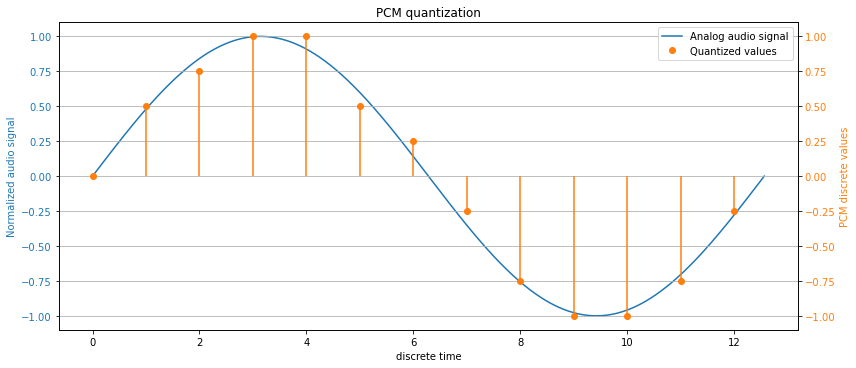
\includegraphics[width=0.9\textwidth]{thesistemplate/fig/pcm_plot.png}
    \caption{PCM quantization example, with linearly uniform quanization levels (LPCM).}
    \label{fig:pcm}
  \end{center}
\end{figure}



\subsection{Mel Frequency Cepstral Coefficients}

The Mel Frequency Cepstral Coefficients (MFCC) are short-term features dominantly used for speech recognition \cite{mfcc_logan2000mel}, speaker identification and proven to be beneficial for general audio processing purposes for Music Analysis or Genre Classification.

Figure \ref{fig:mfcc_proc} shows the process of the computation of the MFCC features for a given audio wave. The method aims to compress the speech-related information from the amplitude spectrum of the signal in a computationally efficient way, also taking into consideration the human perception of speech. The first step is to create fixed-size frames of the audio signal with the help of a windowing function, for speech detection purposes it usually means 20-30 ms wide segments with Hamming window. 
%JUHAA Why? If you mention it, describe it with a bit more details.
Hamming window has proven to reduce spectral leakage effects in the next DFT step \cite{mfcc_logan2000mel}. The leakage, appearance of high-frequency noises, occurs inevitably because of the edges created by framing the signal and the nonzero difference between the ends. The second problem can be thought of as a jump in value if we consider it from a Fourier-transformation point of view, which assumes a periodic extension of the signal.

\begin{figure}[t]
  \begin{center}
    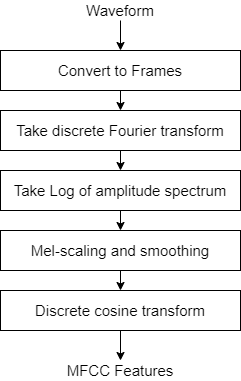
\includegraphics[width=0.25\textwidth]{thesistemplate/fig/mfcc_process.png}
    \caption{Process flow for generating MFCC features from audio signal, adapted from \cite{mfcc_logan2000mel}. }
    % https://ww2.mathworks.cn/help/audio/ref/mfcc.html
    \label{fig:mfcc_proc}
  \end{center}
\end{figure}

This step is followed by the Discrete Fourier Transformation of each frame to get the frequency spectrum representation of the signal from where the logarithm of the amplitude spectrum is extracted next. The logarithm function was applied because human loudness perception follows a quasi logarithmic scale. The phase information is not utilized for MFCC computation, previous research has shown few additional benefits compared to the computational overload.

After the scaled spectrum amplitude components the next step is to reduce the number of components by grouping and averaging them according to the Mel-scale. The Mel-scale is used to divide the whole frequency spectrum to the final number of MFCC bins by dedicating smaller intervals in the lower frequency range and increasing the size in a logarithmic manner mapping the human pitch perception. An example Mel-filter bank for computing 20 mels is depicted in \autoref{fig:mel_filter_bank}.

%JUHAA
% Can you give just a briefly more practical explanation why DCT is applied. The last step here calculates "the spectrum of the log of spectrum", so called cepstrum. It could be done with DFT again but DCT has benefits. See this:
%https://dsp.stackexchange.com/questions/31/how-do-i-interpret-the-dct-step-in-the-mfcc-extraction-process
Finally, a Discrete Cosine Transform (DCT) is applied to decorrelate the Mel-spectral components, increase noise tolerance and produce the final MFCC feature set. DCT is selected in contrast to DFT because the expected shape of the spectrum is a declining line approximately, which is hard to fit with a full cycle of sine waves with DFT, while DCT has cosines with a half-integer number of cycles too, and does not assume periodic extension of the signal. To compress the information but preserve the overall shape of the spectrum, the algorithm discards the higher coefficients and only selects the first (say) 20-40 values of the DCT function as a good representation of the signal.

% http://citeseerx.ist.psu.edu/viewdoc/download?doi=10.1.1.11.9216&rep=rep1&type=pdf
% https://wiki.aalto.fi/display/ITSP/Cepstrum+and+MFCC



\begin{figure}[ht]
  \begin{center}
    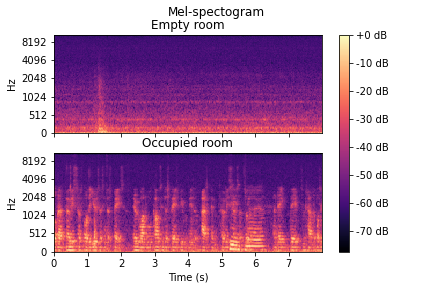
\includegraphics[width=0.8\textwidth]{thesistemplate/fig/mel_spec_comparison_ex.png}
    \caption{Mel-spectogram examples for short empty and occupied room recordings, the upper recording only had small noises from outside, while in the lower case represents an ongoing conversation.}
    \label{fig:mel_comp}
  \end{center}
\end{figure}


\begin{figure}[ht]
  \begin{center}
    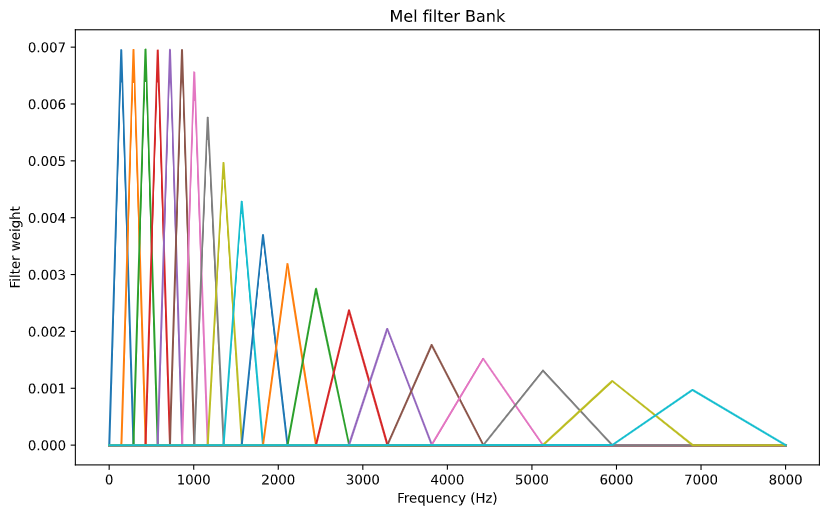
\includegraphics[width=0.8\textwidth]{thesistemplate/fig/mel_filter_bank.png}
    \caption{Mel-filter bank for 20 mels for 16 kHz sampling rate, each triangle represents the weighting values for the entire frequency spectrum, the peaks are constant until 1kHz and it decreases a logarithmic way for higher frequencies mimicking the human perception of sound.}
    \label{fig:mel_filter_bank}
  \end{center}
\end{figure}



 
%  Digital Signal Processing introduction contents:
%  \begin{itemize}
%   \item PCM, sample-rate - ok
%   \item Fourier transformation
%   \item Mel frequency spectrum/ MFCC - ok
%   \item Short time energy (STE), dBFS - decibels relative to full scale
%   \item Windowing, feature engineering
% \end{itemize}




% PDF\@.
% Comment: If your sentence ends in a capital letter, like here, you should
% write \@ before the period; otherwise LaTeX will assume that this is not
% really an end of the sentence and will not put a large enough space after the
% period. That is, LaTeX assumes that you are (for example), enumerating using
% capital roman numerals, like I. do something, II. do something else. In this
% case, the periods do not end the sentence.

% Similarly, if you do need a normal space after a period (instead of
% the longer sentence separator), use \  (backslash and space) after the
% period. Like so: a.\ first item, b.\ second item.



\chapter{Methods}
\label{chapter:methods}
%TODO : Change logo
% \emph{[Supervised machine learning basics, neural networks, convolutional, fully connected layers, Recurrent NN, Model ensemble options (compare it with traditional alg.) ]}
% \bigskip

% JUHAA
% It feels to me that your methods section is somehow lacking the thread. Of course there was still missing parts but more clear connection to your implementation would help to understand it. And you need to explain only main methods you really use. I would try to avoid having short sub sub sections.

% What I try to say is that try to compress your text a bit and add clear links to your implementation. For example “this method is often used with problems that are very similar to the one discussed in the thesis…”


This chapter starts with a theoretical part related to machine learning and Artificial Neural Networks with the concept of Model Ensemble at the end. The theoretical concepts are always supported with typical use cases to help the reader better understand the different approaches.A supervised machine learning framework will be chosen to formulate a generalized model for occupancy detection based on the features extracted from the dataset described in the previous chapter. The presumption is, that by using nonlinear classification methods the speech information can be extracted with higher precision.


\section{Machine Learning introduction}

Machine learning as a subset of Artificial Intelligence research aims to develop algorithms, which performance improves with data given during the learning process. Or as famously known from Tom M. Mitchell: "Machine learning is the study of computer algorithms that allow computer programs to automatically improve through experience" or “A computer program is said to learn from experience E with respect to some class of tasks T and performance measure P, if its performance at tasks in T, as measured by P, improves with experience E” \cite{ML_book_Mitchell97}.

In the next section, the three main branches of machine learning will be introduced briefly, supervised, unsupervised, and reinforcement learning. 


\subsection{Types of Machine Learning tasks}


\subsubsection{Supervised Learning}

In a Supervised Learning setting a dataset is given with the corresponding correct output or so-called label for each example. Starting with a labeled dataset the tasks can be divided into two main categories: classification and regression. In the first case, the machine learning model tries to learn the generalized mapping between the input dataset and the provided labels or classes while in regression the model output is a continuous function \cite{DL_book_Goodfellow}.

\subsubsection{Unsupervised Learning}

Unsupervised learning algorithms aim to extract patterns from data without any a priori information provided such as labels or scores. In clustering, the patterns are used to group samples based on their similarity and, in addition, the clusters can help detecting outliers of a given dataset. The research field dedicated to outlier detection is called anomaly detection and their findings used extensively in several industrial scenarios, in finance for bank fraud detection or in cybersecurity domain for intrusion detection and system health monitoring \cite{DL_book_Goodfellow}. Alternatively, in principal component analysis, the extracted information is used to compress the training dataset by selecting the features which most discriminates the samples from each other and reduce the dimensionality of the problem \cite{DL_book_Goodfellow}.


\subsubsection{Reinforcement Learning}

Reinforcement learning problems are often modeled as for an agent to interact with an environment and take the best action sequence, which maximizes its reward \cite{RL_book_Sutton1998}. Explicit data collection is not needed for the problem in advance in the traditional sense, as the data is most often generated during the learning phase. One key challenge is that the agent has to find the right balance between exploration  of new actions and exploitation of already proven solutions. Board games such as chess and Go are the most recent areas where implementation of RL algorithms turned to be useful for reaching superhuman performance level strategies \cite{silver18alphazero}.

%JUHAA
% Reference for GO chess etc..
% https://discovery.ucl.ac.uk/id/eprint/10069050/1/alphazero_preprint.pdf

\subsubsection*{Discussion on the used approach}
Among the three introduced machine learning paradigm, for our goal, the easiest solution would be to form it as a Supervised Learning challenge. Collecting audio files representing unoccupied and occupied room scenarios and labeling them respectively, gives us a binary classification problem. Building a model aiming to spot the human speech or noises in a given time frame. Moreover, to ensure the usability of the model in various circumstances, the aim is to use the most diverse training sources, cover the most common use cases, and choosing the right architecture for the model, to be able to capture the underlying patterns in the dataset. While the concept of Unsupervised Learning would target to find anomalies or similarities in the dataset without human input, which might mislead the learning process since our target is clearly defined.


\section{Artificial Neural Networks}

Artificial Neural Networks \cite{DL_book_Goodfellow}, in the most general sense, are directed computational graphs with learnable parameters. Early models, such as the Perceptron, were inspired by the structure of the human brain, artificially replicating neurons as universal computational units and synapses to transmit signals across the network. Conventionally, neurons are grouped into layers which perform similar functionality, then layers stacked together to construct the final network.

The main incentive behind the research of Neural Networks is to define mathematical models which can adapt to the task requirements and perform better with experience. Feedforward architectures with nonlinear activation functions can approximate any continuous function according to the Universal Approximation theorem \cite{HORNIK1991univ}, which makes them viable for complex high dimensional problems with the right training algorithms.

\subsection{The Perceptron}

In machine learning, the Perceptron \cite{rosenblatt1958perceptron} was one of the first realizations of an Artificial Neuron, constituted of a weighted sum of its inputs plus the bias term which then forwarded to a thresholding function:


\begin{equation}
      f(x) =
    \begin{cases}
      1 & \text{if $W\cdot x + b > 0$}\\
      0 & \text{otherwise.}
    \end{cases} 
\end{equation}

The $f(x)$ function is an early version of the more complex activation functions used nowadays, it simply implements a step function, therefore the model will output 1 if $x$ was positive and 0 in negative cases. The decision boundary can be adjusted by the $b$ bias term. Therefore if used in single layer configuration it can only converge for linearly separable problems and require a custom training algorithm given that the activation function is not differentiable.

\begin{figure}[ht]
  \begin{center}
    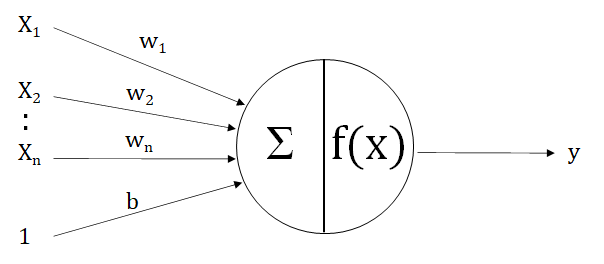
\includegraphics[width=0.7\textwidth]{thesistemplate/images/perc.png}
    \caption{Structural diagram of a Single Perceptron node.}
    \label{fig:perceptron_struct}
  \end{center}
\end{figure}


\subsection{Multi-Layer Perceptron}


In the Multi-Layer Perceptron model (MLP) perceptrons are organized into a layered structure where the input data flows only forward, from the input to the output, hence the alternative name, Feedforward Networks. Alternatively, in recurrent neural networks \cite{sutskever2013training_rnn}, the computation flow contains feedback loops, allowing the model to capture historical information, so the current prediction will not depend only on the current input but the preceding ones, too. It is widely applied to time series data forecasting and natural language processing tasks.

Single-layer Perceptrons can only find viable classification boundaries for linearly separable problems, for non-linearly separable more complex problems multiple-layer setup is needed. 

Neural networks are intended to approximate some ideal function $\hat f$, in the case of classification, $y = \hat f(x)$ where $x$ denotes the input and $y$ is the assigned category for $x$. An MLP aims to find this mapping $y = f(x, \theta)$ by adapting its parameters $\theta$ during the learning process \cite{DL_book_Goodfellow}.

% \begin{align*} 
% z &= W^T x,  \\     
% y  &= \sigma (z)
% \end{align*}

% JUHAA
% What is the reason for this equation, no link to the text

% also with (l) layer number marked in top

\subsection{Convolutional Neural Networks}

Convolutional neural networks (CNN) are a special type of feedforward network, where the weights are shared across the layer and each neuron is only connected to a subset of input elements determined by their locations. It has first gained popularity in Imagenet \cite{deng2009imagenet} Large Scale Visual Recognition challenge for image classification acting as a feature extractor usually in the first part of the network. Stacking several Convolutional layers with nonlinear activation functions together allows the network to extract high-level or abstract information from an image in an automated way, by finding the best low-level features and combining them for the final prediction.

Convolutional Networks can be thought of as feedforward networks that apply convolution instead of matrix multiplication \cite{DL_book_Goodfellow}. The function takes two arguments, the previous layer output as input and a kernel, and outputs a feature map. The kernel is usually one-dimensional for time series data and 2D for image data. The kernel parameters are adapted by the learning algorithm during training. \autoref{fig:cnn_parshare} illustrates the effect of the application of a kernel instead of the dense connections.

Nodes are only connected to the closest ones in the previous layer determined by the kernel size, in contrast to MLP structure where every all of the nodes are connected between two layers. Moreover, instead of learning the weights for each node-node connection, we are sharing the kernel parameters across the layer. Most implementations compute several feature maps with different kernels on the same input, therefore increasing the output tensor dimensions.


\begin{figure}[ht!]
  \begin{center}
    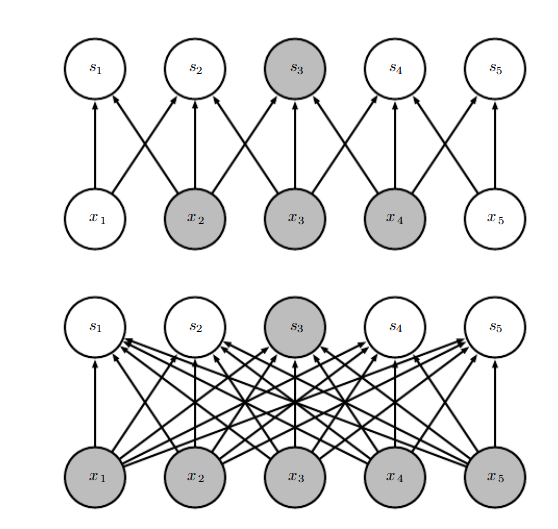
\includegraphics[width=0.5\textwidth]{thesistemplate/images/cnn_sparse.png}
    \caption{Comparison of Convolutional (upper) and Fully connected (lower) layers for parameter sharing, sparse connection is illustrated with arrows and gray coloring on the nodes \cite{DL_book_Goodfellow}.}
    \label{fig:cnn_parshare}
  \end{center}
\end{figure}


The first breakthrough happened in the late 1990s when deep learning had proven to be useful for handwritten character recognition tasks, with a relatively simple 5 layered structure involving only 2 convolutional layers for feature extraction \cite{lecun1998CNN}.

% \begin{itemize}
%     \item TODO: Kernel size, stride, padding image
%     \item TODO: Pooling explanation, max, average
% \end{itemize}

\subsection{Activation functions}

Activation functions as a nonlinear transformation play an important role in Multi-layer neural network modeling. Any combination of linear functions would remain a linear function, so to model nonlinear processes we need to employ nonlinear transformation in the computation \cite{nwankpa2018activation}. Another criteria from a computational point of view is differentiability since for automated learning the gradient must be computed using back-propagation. 

Some of the most commonly used activation functions are visible on \autoref{fig:act_func}. Sigmoid or Logistic function restricts the output to [0,1] interval with the formula given below, which are often used for last layers to output probability. Tanh or hyperbolic tangent exhibits similar characteristics in shape but transforms the input to range [-1,1] symmetrically. However, these functions are subject to the vanishing gradient problem, making the gradient-based learning slow due to the almost zero gradient outside the transitioning middle part. So if the system starts or ends up in those flat sections the parameter updates might be slow and ineffective without additional tricks such as momentum update \cite{QIAN1999145momentum}.

Rectified Linear Unit or shortly ReLU is the most widely used activation function currently, it mitigates the vanishing gradient problem for positive numbers because its gradient is always 1 for every positive input. Even if the gradient is undefined in zero, practical implementations usually substitute f'(0) = 0, which reduces the computational complexity with its simple definition. Further developed solutions includes Leaky ReLU \cite{DBLP:leakyReLU} and  Exponential Linear Unit ELU \cite{clevert2015fast_elu}, as an attempt to allow the learning for negative inputs.

\begin{equation}
    \mathrm{Sigmoid}(x) = \frac{1}{1 + \exp(-x)}
\end{equation}

\begin{equation}
    \mathrm{Tanh}(x) = \frac{\exp(x) - \exp(-x) }{\exp(x) + \exp(-x)}
\end{equation}

\begin{equation}
    \mathrm{ReLU}(x) = max(0,x)
\end{equation}

\begin{figure}[ht]
  \begin{center}
    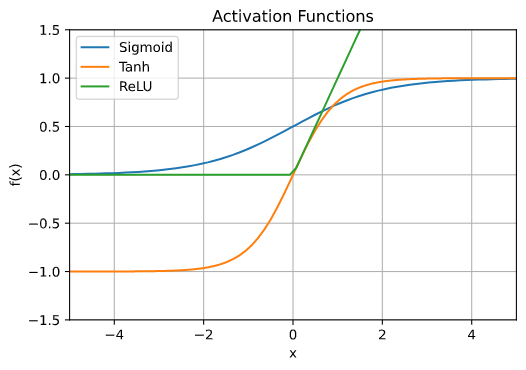
\includegraphics[width=0.58\textwidth]{thesistemplate/fig/activation_funcs.png}
    \caption{Most commonly used activation functions.}
    \label{fig:act_func}
  \end{center}
\end{figure}


% \section{Training techniques}

\section{Regularization techniques}

%JUHAA
% Consider, if you want to use these sub-sub-sub sections. You could have regularization topic only.

This section provides a general overview of the most common methods and concepts for achieving high accuracy values for a supervised machine learning problem. Regularization is a set of tools aiming to reduce the testing error by preventing overfitting the model on the training dataset.

\subsection{Dropout}
The dropout layer randomly sets some of the input tensor elements to zero with a predefined probability $p$ during the training process, which has proven to be useful for avoiding overfitting in various situations \cite{dropout_effect}.
%JUHAA
% Give at least one example

The reason behind eliminating part of the neuron outputs during the learning process is to force to build a more generalized model which is robust even in extreme conditions and helps the neurons to form generalized learning instead of specializing only to recognize one feature.
% https://arxiv.org/pdf/1207.0580.pdf

\subsection{Batch normalization}

%JUHAAA
% Picture with names of the parts of the process would help understanding where normalization takes its place.

A Batch normalization (BN) layer normalizes the output of a layer in a mini-batches during training, as a part of the network structure. Allows having larger learning rates, a more stable training process and reduced dependence on initialization \cite{ioffe2015batch}.

It is usually applied after a fully connected or convolutional layer and before the activation function for maximal efficiency.
%https://arxiv.org/pdf/1502.03167.pdf


% \subsection{Non-Convex Optimization}

% Cross-entropy loss: for binary classification
% \begin{equation}
%     L(x,y) = - \Big[ y\log(x) + (1-y)\log(1-x) \Big],
% \end{equation}
% where $x$ denotes the model output, while $y$ represents the target.

% Backpropagation: is a nonlinear optimization method for minimising the loss function by updating the parameters of the neural network.

% contents:
% \begin{itemize}
%     \item loss functions, binary cross-entropy in our case
%     \item backpropagation
%     \item gradient descent, momentum    %https://arxiv.org/abs/1609.04747   -   An overview of gradient descent optimization algorithms
%     \item optimizers, Adam \cite{kingma2017adam}
% \end{itemize}


\section{Model Ensemble}

% \emph{[Theoretical intro, block diagram of the prediction model]}

The high-level concept of the multisensor presence detector is to find a viable framework and building blocks for synchronizing the different sensor inputs and extracted predictions into one unified room occupancy state. Our work is focusing on only binary classification, to differentiate between empty and occupied office meeting room scenarios. Although initial research suggests that from the analog audio and PIR signals more information could be inferred like crowd size, identification of participants age, mood, we leave that for future research options and discuss it more in detail in Chapter \ref{chapter:discussion}, because it is just partially related to our topic.

Choosing a model ensemble approach was an early architectural design decision influenced by multiple factors. Previous research reports deploying single supervised ML models on top of multidimensional data collected from different environmental sensors (see Section \ref{section:Multisensor_research}), but the data collection is usually restricted only to one office room. These datasets are inherently carrying the special usage behaviors of the workers together with the unique arrangement of sensors, which can be misleading for developing a general occupancy prediction model expected to work in multiple different scenarios. The research field is currently lacking a reliable and diverse training dataset covering multiple locations and sensory inputs. The problem is even more visible with the audio or noise level information. To make the model more robust we tried to aim to use as many training examples as possible, but selecting only the ones where both audio and PIR information is available for the same room we would have limited ourselves to recordings from our office exclusively. Therefore, models dedicated for audio and PIR were separately trained, and in a third block the predictions were merged into one final decision. A high level overview of the multi-model topology is reported in \autoref{fig:multisens_pred_proc}.

%JUHAA
% No reference for this image in the text
\begin{figure}[ht!]
  \begin{center}
    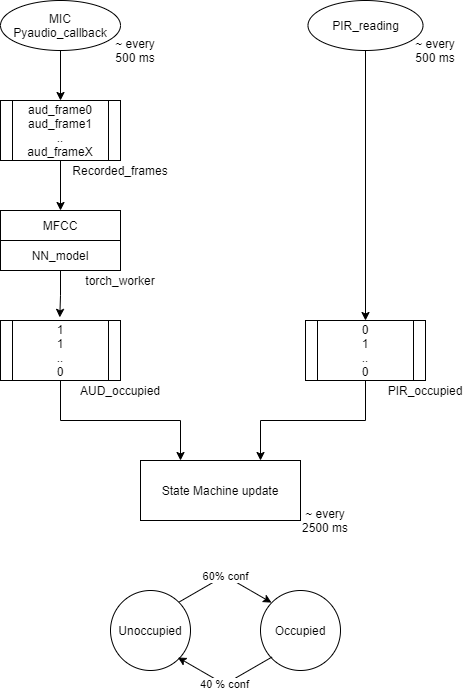
\includegraphics[width=0.58\textwidth]{thesistemplate/fig/multisensor_uml.png}
    \caption{Multisensor prediction process on the Raspberry Pi 4B platform.}
    \label{fig:multisens_pred_proc}
  \end{center}
\end{figure}

\section{Embedded AI development process}

Developing machine learning algorithms with embedded deployment generally imposes additional constraints on the process, due to the hard limitations of the selected hardware platform. An overview of the followed workflow can be seen in Figure \ref{fig:embAI_workflow} down below. As in most embedded AI projects, the dataset manipulation and neural network training steps are implemented in a regular desktop PC environment while the embedded platform is only used to run the inference with the already trained network parameters for testing purposes. In the next section, we will follow through each step to create a binary classification model for human presence detection based on sound. 

Starting with target selection, we present methods and design choices with reasoning for data collection and labeling. The careful selection of data sources is crucial for a positive outcome, it fundamentally defines and limits the theoretical capabilities of the model. In the preprocessing step we will generate the input for the training by windowing the audio signal and computing the selected MFCC features and reshaping them into a 2D matrix. This section is followed by several model training with grid search. The best-performing models which meet the computational limitations of the embedded platform get selected and converted to C arrays and libraries. Finally, the supporting functionality will be implemented which bridge the gap between the sensors and the machine learning model input, namely interfacing and feature extraction.



% https://arxiv.org/pdf/1911.03314.pdf

% TODO: change the line to model conversion to embedded platform
\begin{figure}[ht!]
  \begin{center}
    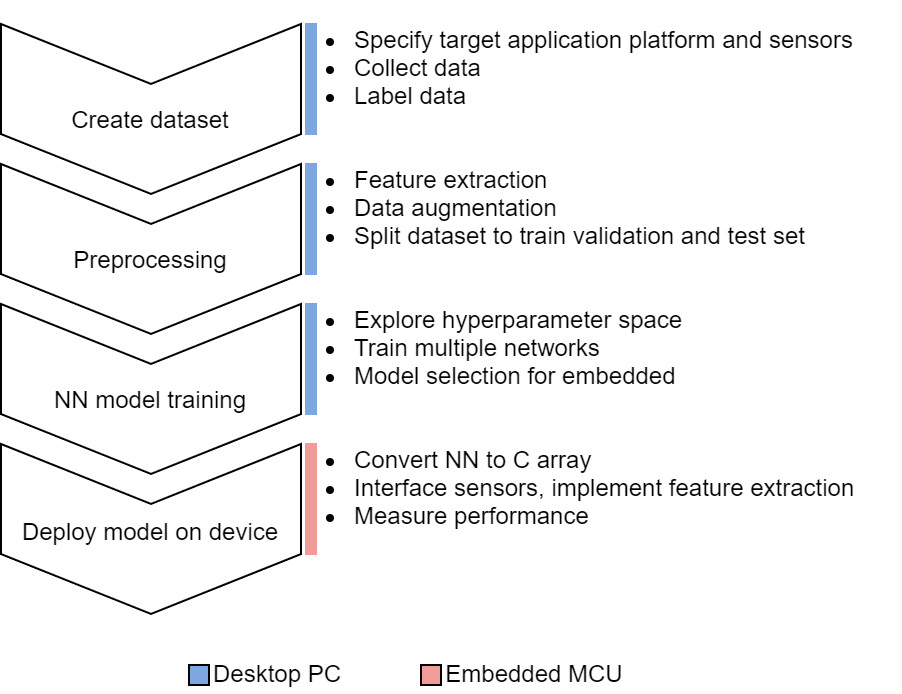
\includegraphics[width=0.75\textwidth]{thesistemplate/images/embAI_process.png}
    \caption{Embedded AI development workflow, adapted from \cite{wang2020fannonmcu}.}
    \label{fig:embAI_workflow}
  \end{center}
\end{figure}



%#################################################################################################################
%#################################################################################################################

\chapter{Audio based presence detection}

In this work, we had to make an arbitrary design decision early on, related to the focus of the ideal capabilities of the machine learning model, given the limited amount of computational resource for inference and helping the testing process, considering only the most typical use cases. Therefore our target is to recognize the human presence in the audio flow mostly based on speech and partially based on other additional noises such as placing and moving objects on a desk. 


By stating this early on the project will allow us to collect data to specifically cover these situations together with additional publicly available datasources, for a supervised machine learning classification setup.


%The audio sensors can pick up even the smallest noises in a silent room like keyboard typing or breathing as an indication of human presence, but in meeting rooms speech is the easiest marker to detect due to the relative loudness compare to the background noise and the characteristic frequencies people use to communicate.

\section{Data collection and analysis}

A large, diversified dataset is essential for any kind of machine learning problem. Given our final goal to test and run the model in real-time on an embedded platform with a certain digital microphone, we have collected data also with the same hardware tools used in the implementation. Moreover, we have used subsets of large publicly available datasets for extending the training set, leading to a more generalized model. First, the data collection approach will be elaborated with special attention to the used hardware and environmental choices for recording. This will be followed by the external audio sources selected for training. Finally, a summary will close the section, where all the different audio files are categorized and grouped into a condensed table.

Given the problem definition, the desired behavior for the audio-based machine learning algorithm is to distinguish between human presence and empty room scenarios from the audio feed. This frames the task as a binary classification, and to construct a proper dataset we need to collect data for both cases and label them for the training.


\subsection{Field Data collection}

For easy and quick data collection on-site, we have utilized a Raspberry Pi 4B with the same MEMS microphone used in the implementation (see  \autoref{subsub:Aud_sensor}). Fortunately, the Raspberry Pi board can interface the audio mic with the same I2S bus as the microcontroller and with the help of well documented high-level libraries made the data collection and the initial model testing fairly convenient. All audio was recorded with 16kHz to match with the target for the implementation. 

In the case of an occupied room, we placed the setup into a relatively large open office space and recorded short pieces of conversation with the approval of the people present at that time. Usually, the recording equipment was placed at a desk in the middle of the room, while employees had a casual talk next to it. But due to the cumbersome process for requesting consent and often empty offices, most of the speech data was borrowed from external sources. The condensed speech recording sums up 10 minutes in total.

While for representing unoccupied rooms, the sensor was placed in various empty meeting rooms on-site with the purpose to record not only the silence therefore the microphone inherent noise but also noises related to activities outside the examined room. These include environmental noises caused by wind, rain moreover attenuated speech, cars, or other noises coming through windows and closed doors. Additionally, a private apartment was used for collecting data representing environments with a higher background noise level. The apartment had windows open and closed while cars were passing by in front of it. Furthermore in random intervals construction noises made the recording more diverse due to renovation in the building. The manual recordings related to the empty room class altogether reach two hours in duration.


\begin{figure}[ht]
  \begin{center}
    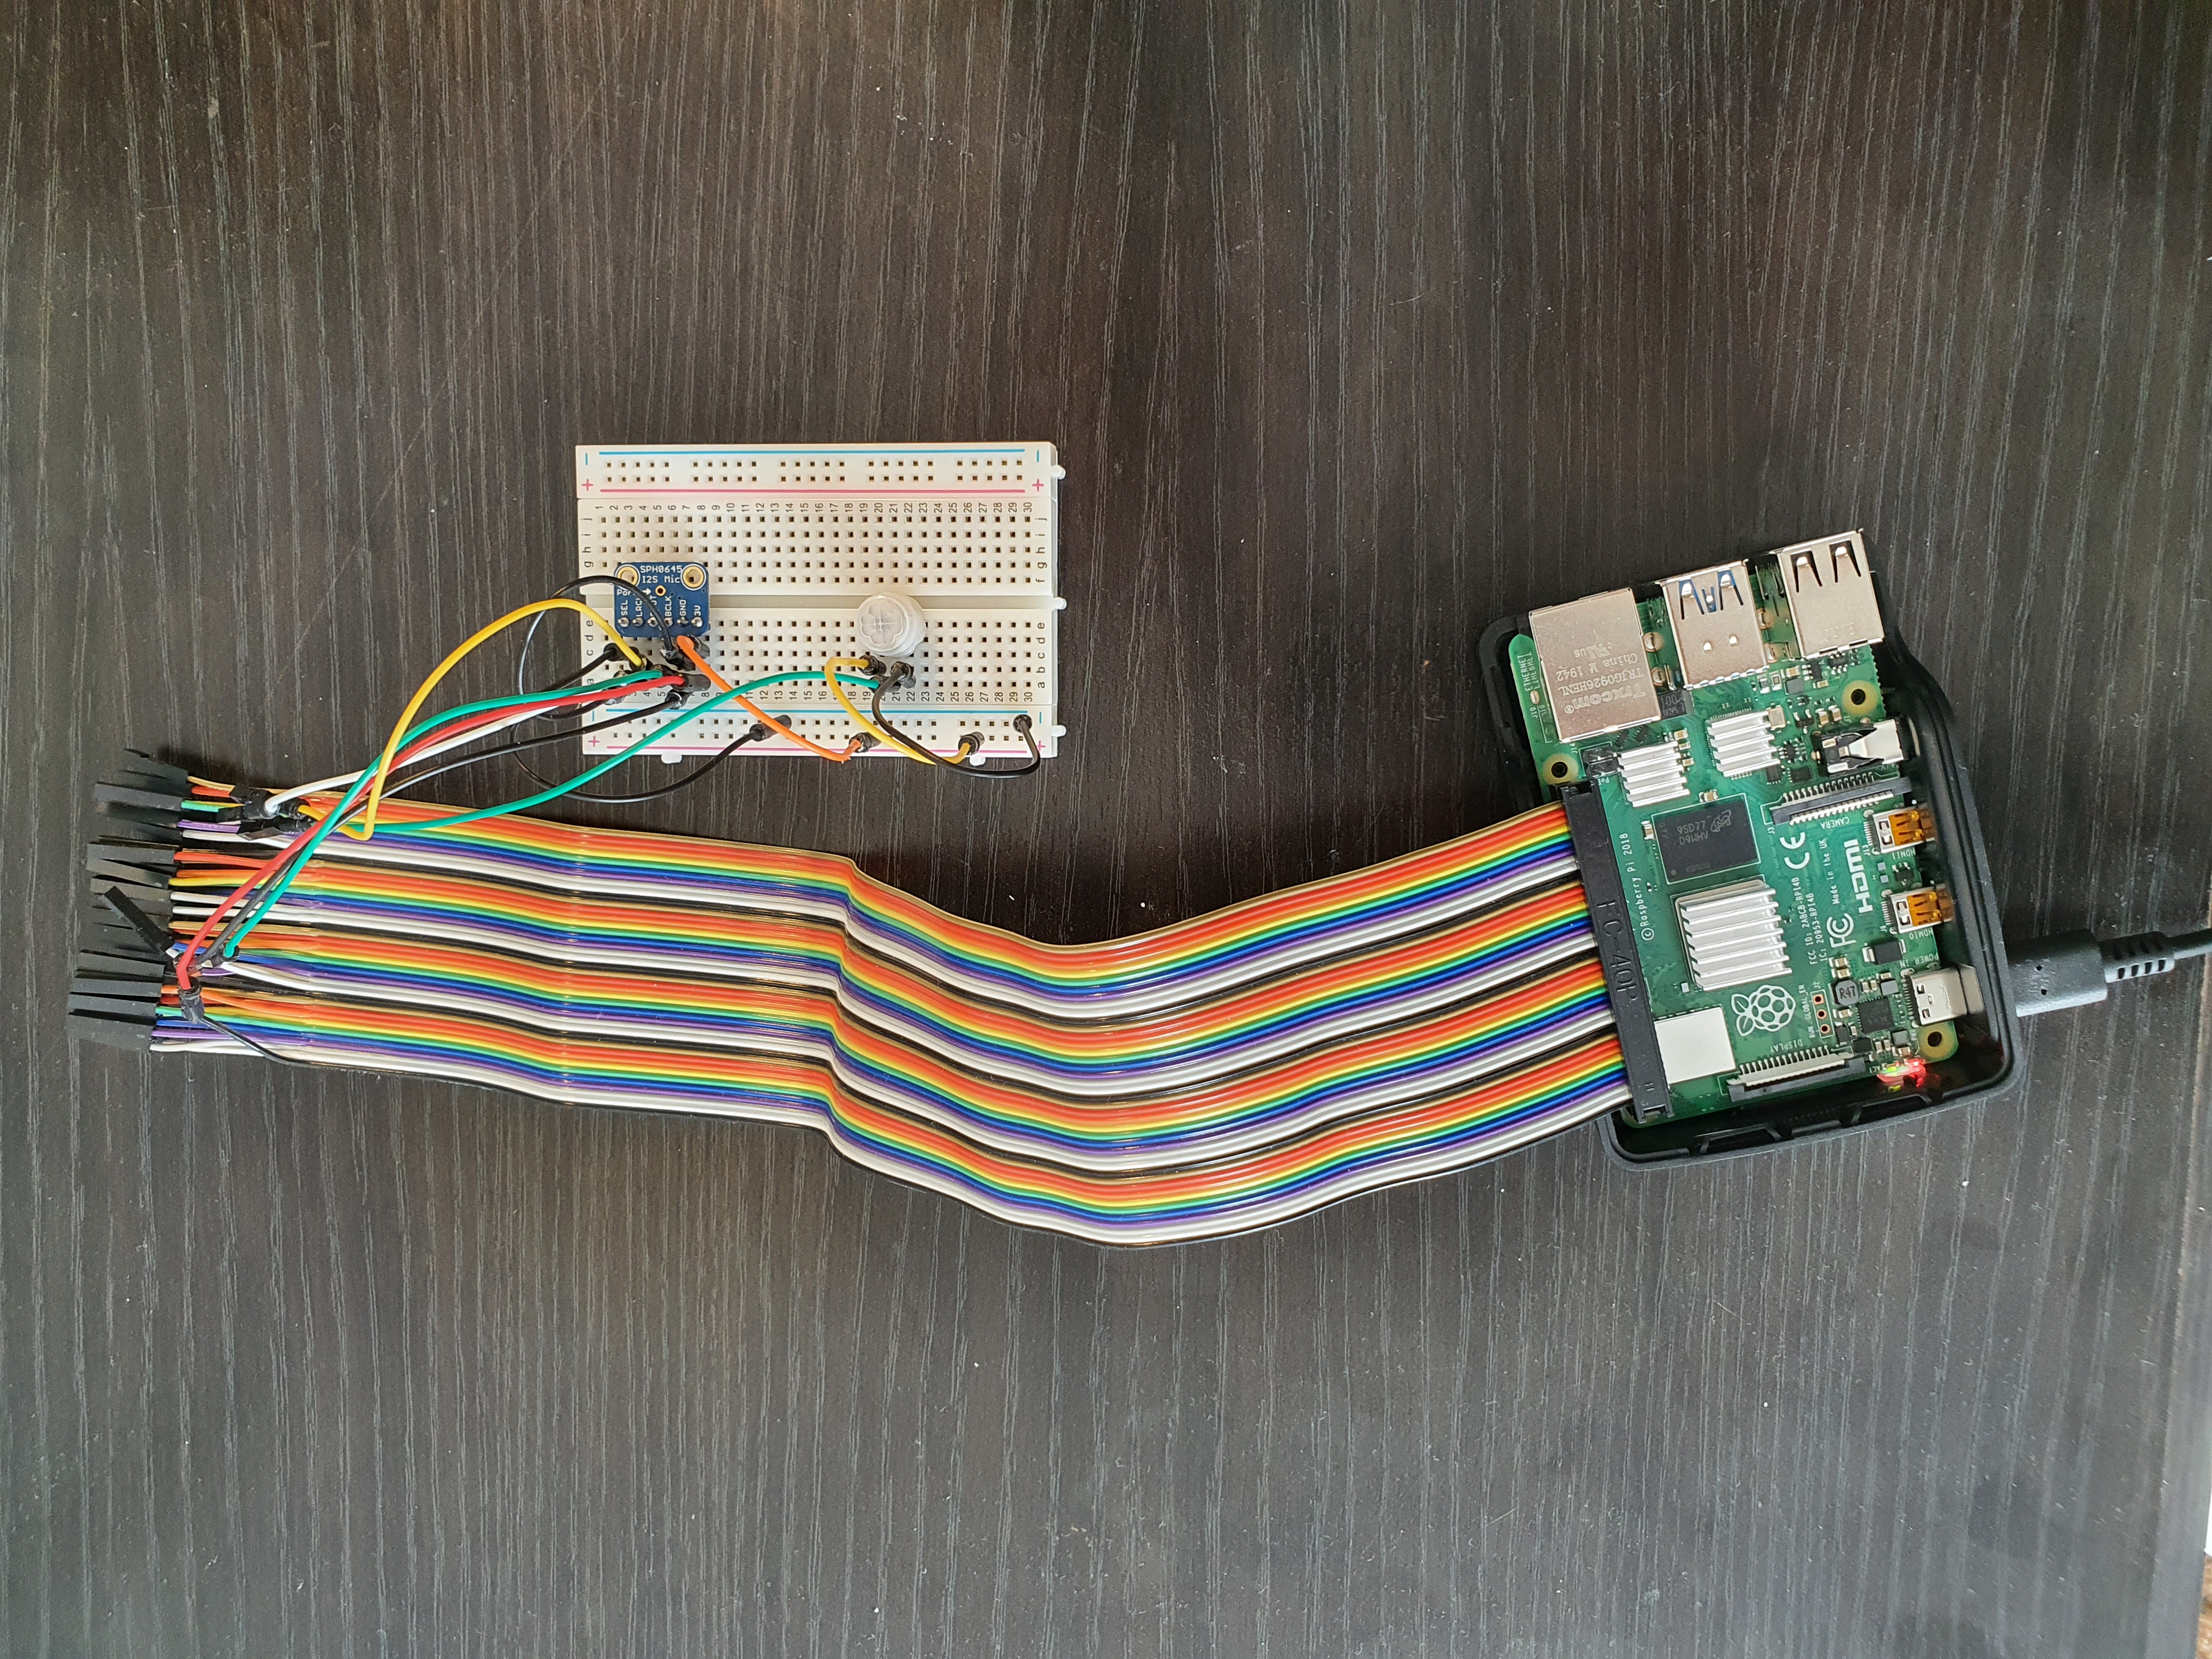
\includegraphics[width=0.6\textwidth]{thesistemplate/images/rpi_setup.jpg}
    \caption{Raspberry Pi 4B data collection setup with digital PIR and Sound sensors.}
    \label{fig:rpi_coll}
  \end{center}
\end{figure}

\subsection{External Data sources}

Since our aim is mostly voice activity detection, for that purpose many large, high quality, and diverse audio datasets are available for training purposes. During the selection process, our objective was to find human speech and background noises most similar to the test scenarios.

\paragraph*{Librispeech}\cite{librispch} is a publicly available corpus for Automatic Speech Recognition (ASR) derived from English audiobooks summing up to 1000 hours of speech by 2500 participants usually in background noise free environments. The audio is sampled at 16kHz and provided under the CC BY 4.0 license. Although the dataset is immense and the size is justified for speech recognition tasks we only used the dev-clean subset, a few hours of data produced by a total of 40 speakers. Clean refers to lower Word Error Rate (WER) speakers, meaning their speech was easier to decode with a baseline algorithm trained on WSJ (Wall Street Journal) dataset. Librispeech was used exclusively as a representation of occupied room state, can be viewed as a simulated conversation.

\paragraph*{QUT-NOISE} \cite{qut_noise} is a collection of background noises categorized into five different scenarios; CAFE, HOME, STREET, CAR, REVERB, in a total of 10 hours. After listening to short parts of each category, in the HOME segment, HOME-KITCHEN were selected as occupied room state, while CAR as unoccupied. HOME-KITCHEN as indicated in the title was recorded in a kitchen, during some sort of food preparation most probably. It was selected to make the learning more robust and able to spot non-speech-based human presence. In CAR scenario, researchers were collected street noise while driving, and it resembled most of the outdoor noises one would expect as background noise in a meeting room next to a street. All the samples were recorded at a 48 kHz sample rate and the data is publicly available under the CC-BY-SA license. The selected HOME recording is around 35 minutes long while the CAR scenario takes 130 minutes.


\paragraph*{Generated Noise} samples. Several noise samples were added to the training set simulating the self-noise of the selected microphone or monotonic noises present in indoor spaces produced by HVAC or other electronic devices. The selected noise profiles are white and red (Brownian) noise, after empirical testing of the perceived sound. White noise has approximately equal intensity across the different frequencies while red noise has the energy focused on longer wavelengths (smaller frequencies) and decreasing towards higher frequencies, analogously to the electromagnetic spectrum of the red light. A total of 35 minutes of sound was produced in this way.

% \begin{itemize}
%     \item Plot frequency spectrum of the white and the red noise if you really have too much free time
% \end{itemize}

\subsection{Summary of the training dataset}

 Overall, the whole constructed dataset consists of 12 hours of audio approximately. During the data collection, we paid special attention to represent the most typical use cases that might appear in an office environment while keeping the quantity of the two classes in balance. The different sources and their corresponding audio length are summarised in \autoref{tab:aud_database_sum} below.
\begin{table}[ht]
\centering
\begin{tabular}[t]{|l|l|r|}
\hline
\textbf{Category}           &   \textbf{Source}             & \textbf{Length (min:s)}\\
\hline
\multirow{4}{*}{Occupied}   &   Librispeech, dev-clean      &  323:16\\
                            &   QUT-Noise, home-kitchen     &   33:09\\
                            &   Open office (Rec.)          &   10:00\\
\cline{2-3}
                            &   \textbf{Total:}             &  \textbf{366:25}\\
\hline
\multirow{5}{*}{Unoccupied} &   QUT-Noise, car-window        &  130:56\\
                            &   Empty room (Rec.)           &   121:45\\
                            &   Air Conditioner noise       &   60:00\\
                            &   Generated noise             &   35:00\\
\cline{2-3}
                            &   \textbf{Total:}             &  \textbf{347:41}\\
\hline
\end{tabular}
\caption{Summary of the audio database.}
\label{tab:aud_database_sum}
\end{table}%




%Contents:
%\begin{itemize}
%  \item Data collection with Raspberry Pi 4B, time duration, empty meeting room, open office situations - ok
%  \item External audio souces, Librispeech \cite{librispch}, QUT-NOISE \cite{qut_noise}, white noise - ok, maybe ESC-50
%  \item reasoning about the 16k Sample Rate, previous studies, industry actors... - okayish
%  \item distribution of the dataset for training - ok
%\end{itemize}

% other audio datasets
% https://pytorch.org/audio/stable/datasets.html
% https://research.qut.edu.au/saivt/databases/qut-noise-databases-and-protocols/
% https://eprints.qut.edu.au/38144/1/c38144.pdf
% https://www.openslr.org/12
% https://commonvoice.mozilla.org/en



\section{Data loading and resampling}

As a first preparation step for data processing, we are loading each audio file to memory with a unified target sample rate of 16 kHz. A subset of the dataset was recorded with a different sampling rate, mostly with 48kHz, which needed to be filtered and resampled to the new target using a high-quality Kaiser window with 64 zero-crossings.
%https://resampy.readthedocs.io/en/0.1.5/api.html

The 16 kHz sampling rate and the Nyquist theorem imply that in our analysis the sampled signal can represent frequencies up to 8KHz correctly. The fastest and computationally most efficient VADs such as the Google WebRTC implementation uses only 8 kHz as a sampling frequency leaving them with only 4 kHz bandwidth for speech detection. However, apart from the resource-constrained implementations, higher sampling frequencies are leading to better results especially from a noise tolerance point of view. Moreover, human speech has frequency components higher than 4 kHz, and the richer representation could allow more sophisticated and robust behavior from the model.

% https://www.dpamicrophones.com/mic-university/facts-about-speech-intelligibility

After looking at the time series audio signal profiles, a relatively large offset can be observed in the signals recorded manually using the Raspberry Pi platform with the MEMS microphone. Regular recordings used from other sources do not have this feature. The phenomenon is due to the physical properties of the device (explained more in detail in \autoref{subsub:Aud_sensor}) and needs to be removed to reduce classification bias, not to mislead the training algorithm. Since all the recordings from the selected MEMS microphone have a constant DC offset, audio files were normalized to zero mean at this step, while in the embedded implementation a DC blocking filter will be applied (see \autoref{subsub:dc_blocking}).

% \begin{itemize}
%     \item TODO: Histogram on the time series data from mic and external, and after the DC was removed
% \end{itemize}

\section{Slicing and labeling}

In the slicing step, we need to determine the window size, which will be the basis of the feature extraction and directly influences the responsiveness of the final machine learning model in real-time inference, since we need to aggregate at least one window of data to calculate the features for prediction. Fixed input size is required for feed-forward neural networks hence the predetermined window size, and in the next steps, one set of extracted features corresponding to one windowed audio signal will be the basis for the model output.

All the data were sliced into 500 ms pieces with zero overlap, the label automatically added based on which category the audio file belonged to during data collection. As an industry-standard most VAD systems are operating with 20-30 ms of audio for one prediction allowing one to experience instantaneous feedback given the low delay, but just long enough to determine the presence of speech. The however larger window size can lead to increased confidence in the prediction given that the system has more data to consider. The loss in the response time is not considered critical at this scale, since the delay timers controlling the luminaries have values in the range of 10-45 minutes. 

Loosen the requirements and increase the window size to 500 ms have an additional indirect benefit with regards to the training process. It makes the labeling easier, assuming that the speech data does not contain long pauses, which would mislead the training. In the case of the Librispeech, the audio was split in every situation when a silence longer than 300 ms were detected, aiming to divide the source into sentences, so the final training set does not contain long periods of silence. On the other hand for environmental noises, we do not face this issue since the sound profile is monotonic. 

\section{Feature extraction}

In the last preprocessing step before the neural network training, we are transforming the audio slices from the time domain to the frequency domain with the help of Short Term Fourier Transformation to finally get the set of MFCC features representing the signal. Starting from 500 ms of audio (8000 elements) an FFT with the size of 512 will create 16 spectrum sections each representing around 30 ms of audio. From each spectrum computed 21 Mel-frequency cepstral coefficients are extracted, from which the first one will get discarded, leaving a total of 20 by 16 elements matrix. \autoref{fig:mfcc_img_comp} shows one representative 2D array example for each class. The first MFCC feature has been discarded in many projects, it usually corresponds to the signal energy or DC component which we do not wish to embed in the model decision process. Human speech should be spotted regardless of the sound volume.

The number of MFCCs extracted varies greatly in recent research works, earlier solutions with lower sampling rates usually compute 9-13 features, while newer versions can go as high as 20 or 40. The area of use influences the design choice by great detail. In Environmental Scene Classification and Automatic Speech Recognition, given these problems are more complex than Voice Activity Detection, require more information, and often use a high sampling rate (48 kHz) with 40 MFCC sometimes combined with Delta and Delta-Delta features. Delta and Delta-Delta are the first and second derivatives of the MFCC series. Other, more primitive methods include Zero Crossing Rate (ZCR) and Short-Term Energy (STE) computation on the time-series signal but these approaches are generally performing poorly in noisy environments and cannot distinguish between different sound sources, only noise levels.


\begin{figure}[ht!]
  \begin{center}
    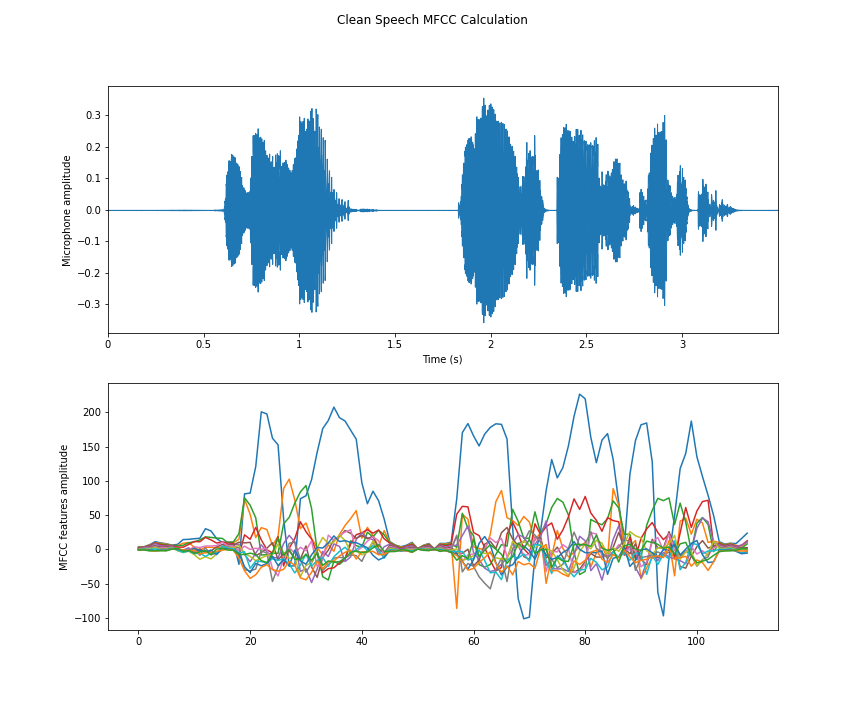
\includegraphics[width=1\textwidth]{thesistemplate/fig/mfcc_timeseries_comp.png}
    \caption{Normalized audio signal and the first 15 MFCC features for a short speech sample, the zeroth MFCC excluded from the plot.}
    \label{fig:mfcc_time_comp}
  \end{center}
\end{figure}

Research shows that it is viable to feed the time series data directly to a deep recurrent neural network for voice activity detection purposes, although it requires a significantly more complicated network structure, therefore higher computational and memory needs. Given our low-performance microcontroller target, striving for the most efficient implementation is key for real-time inference. Optimized Fast Fourier Transformation (FFT) algorithms are widely available for this purpose for most ARM platforms.

The feature extraction and the following section on neural network training have been conducted in python, which is the most popular and well-supported platform for neural network development. MFCC and most audio-related data manipulations utilized the rich functionalities of multiple python packages, most importantly Librosa and NumPy. Librosa \cite{librosa} is one of the most widely used libraries for audio manipulation and analysis, while NumPy \cite{harris2020NumPy} is a general-purpose library for array manipulation and efficient numeric computations.



\begin{figure}[ht!]
  \begin{center}
    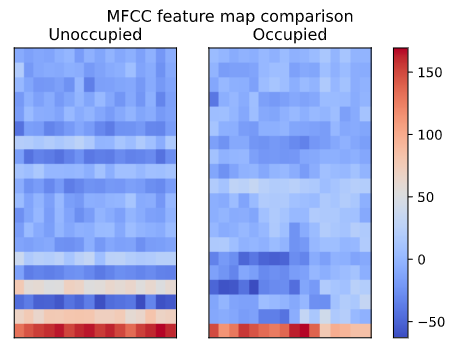
\includegraphics[width=0.6\textwidth]{thesistemplate/fig/mfcc_comp_ex2.png}
    \caption{Comparison of two MFCC image samples from different classes.}
    \label{fig:mfcc_img_comp}
  \end{center}
\end{figure}

Two-dimensional visualization of the dataset after the feature extraction can be seen at \autoref{fig:umap}. Apart from the aesthetic view, data visualization can help to formulate a sense of the problem complexity for classification. The plot can demonstrate the complexity of the problem, given that the task of the learning algorithm is to find the decision boundaries between the clusters of data. The different clusters with the same color show the similarity between elements computed from the same datasource but the clear difference between different sources. The UMAP algorithm \cite{2018arXivUMAP} reduced the 320 dimension input image (20$\times$16) to a two-dimensional representation aiming to preserve the relative differences between elements.



\begin{figure}[ht]
  \begin{center}
    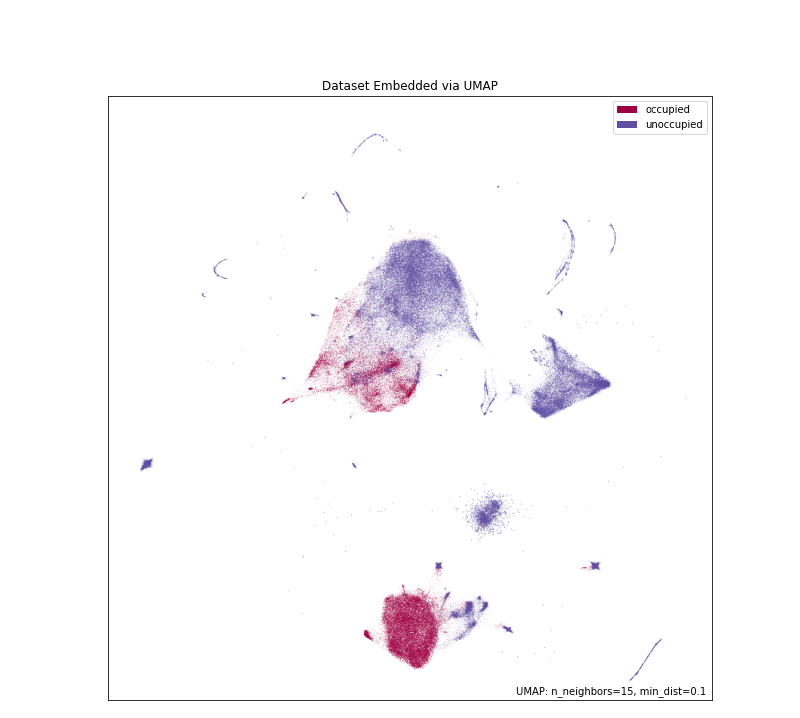
\includegraphics[width=0.8\textwidth]{thesistemplate/fig/umap.png}
    \caption{Visualization of the audio dataset with dimension reduction using UMAP (Uniform Manifold Approximation and Projection \cite{2018arXivUMAP}).  }
    \label{fig:umap}
  \end{center}
\end{figure}


\section{Neural Network design}

The input of the network is fixed to a 20 by 16 two-dimensional matrix of MFCC features, representing 500 ms of audio, while the output is the classification probability for the two classes, occupied and unoccupied room. Labels for all the training data are assigned, making it a fully supervised machine learning problem. Data representing occupied meeting room has 1, unoccupied 0 as a label, which simplifies the calculation of the loss function. The model therefore will have a fixed input size of 20$\times$16 with 2 output nodes each representing the prediction probability that a given input belongs to one of the predefined classes. 

Following a common practice in Data science, the whole dataset was first divided up into three subsets, training, validation, and test set, with ratios of 70\%, 15\%, and 15\% respectively.


Due to limitations of the target hardware and lack of software library support for embedded systems, this work restricts the network structure experiments to feed-forward neural networks only by using fully-connected and convolutional layers as main building blocks and discards more advanced methods such as transformers or recurrent neural networks in general. Recurrent neural networks have the advantage to encapsulate temporal information of the data flow although it usually generates harder training problems and slower convergence. Aggregating the features for longer and then feed them to the network is an alternative to preserve at least partially the temporal characteristics of the input signal at the expense of additional delay. Taking this compromise will allow us to develop solutions based on convolution and linear transformation layers, which efficient implementation exists for most microcontroller platforms.

Additionally, the machine learning framework has to be chosen carefully, given that at some point after the training the models need to be transferred to most probably an Embedded C environment, which might raise some compatibility issues or complicates the prototyping process unnecessarily. The development started with PyTorch \cite{NEURIPS2019Pytorch} but during the first early tests, we have faced great difficulty using the saved model file or converting it to other formats such as ONNX (Open Neural Network Exchange) \cite{bai2019onnx} without success. Unfortunately, at the time of this thesis Embedded machine learning as a field is still in an immature early state and most libraries provide only limited functionality. Although looking for alternatives again now from an embedded inference point of view TensorFlow \cite{tensorflow2015-whitepaper} has made a significant amount of effort to enable the embedded application of their well-established platform. TensorFlow Lite and TensorFlow Lite for Microcontrollers are their solutions for mobile and IoT edge devices for on-device inference. Moreover, Tensorflow Keras \cite{chollet2015keras} provides a simple API interface for most functionality of the TensorFlow framework, therefore in the next sections we will use Keras exclusively as the main Python library for implementing various models.

During the experimentation step for the best neural network architecture and hyperparameter tuning, our main objectives were the highest accuracy on the test set with the least network parameters needed. Tests showed that the number of parameters in the network is directly correlated to the amount of computation i.e. floating number operations (FLOPs) required to run the inference. This is an important observation since our target platform is limited both in memory and CPU power. 

\section{Model architecture optimization}

Finding the best possible layer structure and hyperparameter settings can be highly challenging even for simple problems given the high dimensionality of the optimization, the multimodality of the loss function, and the inherent randomness of the training process. Starting with the same parameters the outcome could be radically different for multiple runs. Considering the high-dimensional search space we needed to make educated guesses on the importance of the different aspects of the training, focusing on a few key metrics while keeping other less relevant details in the same setting. The model optimization had been conducted in multiple exhaustive grid search manners, mostly looking for the best architectural choices but also examining the effect of multiple training setup options.

All the training experiments shared a few properties. Categorical cross-entropy loss was used to measure the performance of the model, and the basis for adjusting the parameters automatically based on the discrepancy using backpropagation and Adam optimizer. The initial learning rate was set to 5e-4 with a batch size of 512. ReLU activation function was selected for all occasions except for the last layer where the Softmax function was applied. The Softmax function takes the input tensor and rescales it that each element will lie in between zero and one and the sum of the values add up to one. Thus the network output can be treated as a probability distribution over the predicted classes, which makes it ideal for comparing the output with the target labels using cross-entropy loss.


\begin{equation}
    Softmax(x_i) = \frac{\exp(x_i)}{\sum_{j}^{ }\exp(x_j))}
\end{equation}

The number of epochs was set to four in all tests to allow fair comparison between the different models. One epoch means one iteration through the entire training set during the training process. The relatively low epoch number was selected in a heuristic manner, models with more epochs were prone to overfitting or predicting constantly one of the labels in real-time testing. The good results even with such a low number of epochs are feasible only because of the small network architectures with a few tens of thousands of parameters and fairly simple problem definition with the constructed dataset.

There were two testing measures applied, and during the experimentation both of them will be reported on the graphs. The first is the traditional prediction accuracy performed on the test set and the second is the result of a short Voice Activity Detection test simulated with short new recordings from the target microphone directly. The new test samples were labeled with the Google WebRTC VAD implementation, and the model performance was measured against those labels. The test audio file takes only a few minutes and was recorded with one speaker in a low background noise environment. It is relatively easy to detect presence even just looking at the raw audio signal but it turned to be useful to test the models also in this way since many of the test cases performed well on the test dataset but produced many unexpected mostly false-positive predictions during the real-world test. The introduction of this audio test shortened the testing process by a significant amount and gave a great tool for detecting overfitting.

\begin{figure}[ht]
  \begin{center}
    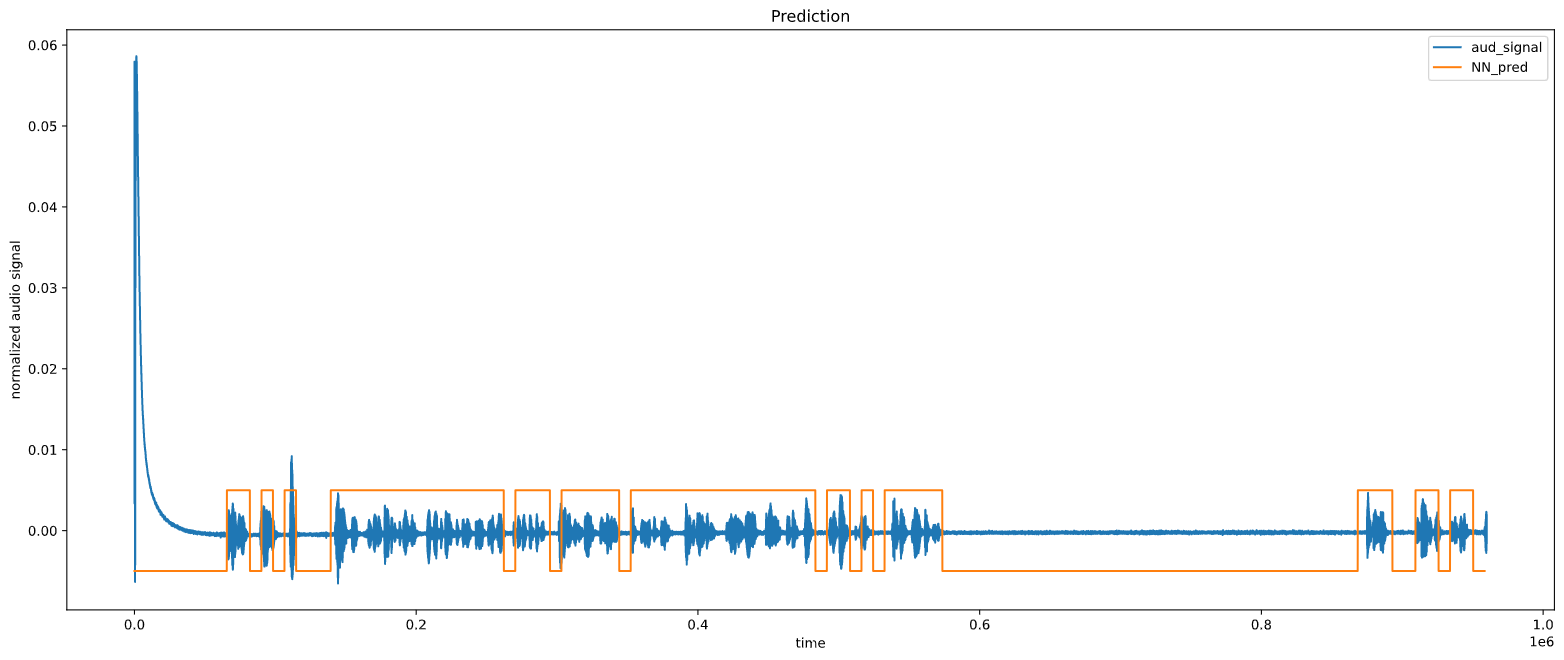
\includegraphics[width=1\textwidth]{thesistemplate/fig/signal_and_pred.png}
    \caption{Correctly functioning model prediction output with clean speech signal.}
    \label{fig:wave_and_pred}
  \end{center}
\end{figure}



\subsection{Fully Connected Neural Network experiments}

The overall structure of the fully connected networks presented in this thesis is summarised at \autoref{fig:FC_structure} below. The custom-developed flexible Python class definition allows us to generate models with different properties while keeping the same structure. Batch Normalization layers can be switched on or off altogether, while the effect of Dropout layers can be regulated with the dropout rate values between 0 and 1. Providing 0 as a probability will change the layer to identity transformation, leaving all the input values intact and forwarding it to the next layer. In most cases when dropout was used the ratio was set to 50\%.

The model architecture starts with the application of a Flatten layer, which was necessary to transform the two-dimensional input to only a list of numbers since the Linear layer only accepts one-dimensional input. This step will make the FCN and CNN models fully compatible and interchangeable, given that their input and output shapes are matching.

The relative position of the Batch Normalization layer in the network varies in recent research. The original Batch Normalization paper \cite{ioffe2015batch} and the first ResNet \cite{he2015deep_resnet} architecture suggest to place the BN layer between the linear and ReLU layers (Conv, BN, ReLU) to maximise the effect of the activation function, where ResNet-v2 paper \cite{he2016identity_resnet_v2} propose alternatives where in some situation BN after the activation function (Conv, ReLU, BN) also lead to improved results in different circumstances. After a few trials, the first arrangement of layers provided a more stable training result, therefore that part will be fixed throughout the experimentation.
% https://forums.fast.ai/t/where-should-i-place-the-batch-normalization-layer-s/56825/4
% and  Gülçehre \& Bengio \cite{ghre2013knowledge_bn_after_relu}


The number of classifier blocks is a configurable property of the model, moreover, the width of each linear layer (the number of neurons)  inside a block is a free parameter too. The only fixed linear layer is the last one called Head in the image with two neurons. This is to ensure compatibility with the labeling of the training data, one for each class. However, since linear layers have significantly larger parameter requirements than Convolutional layers, it limits its usability if not designed carefully. \autoref{fig:FC_1layer} demonstrates that even one wide layer of 512 neurons used after the input has a parameter need around 160000 floating-point numbers which exceeds 1MB of model size when saved. In the Supervised machine learning training context it is not rare to have models taking up multiple gigabytes of space, but in our case, larger models restrict the embedded platform options by a large amount or force to select an unnecessary expensive device for the purpose.


\begin{figure}[ht!]
  \begin{center}
    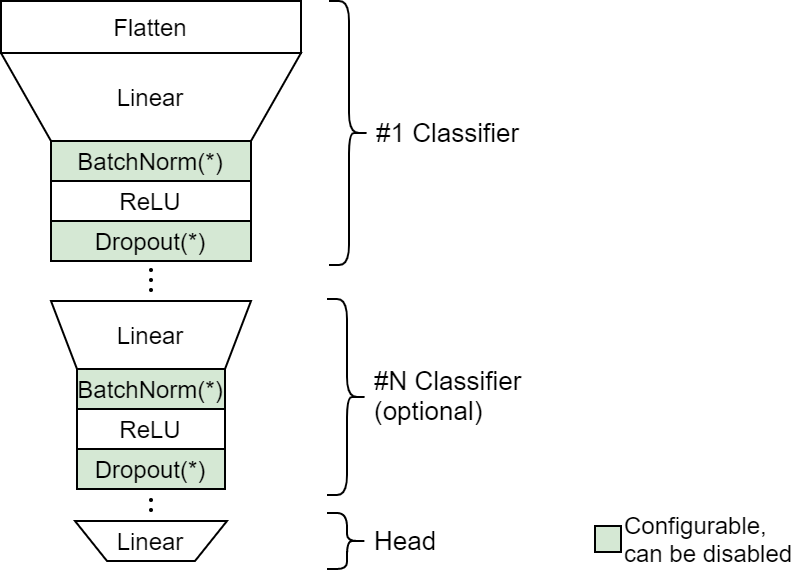
\includegraphics[width=0.7\textwidth]{thesistemplate/images/nn_layer_st_fcn.png}
    \caption{Flexible Fully Connected Network layer structure, additional classifier blocks can extend the model, Batch Normalization and Dropout layers can be turned off.}
    \label{fig:FC_structure}
  \end{center}
\end{figure}


The model names visible in graphs are coding the architectural choices for ease of identification. The layout follows a predefined pattern:

\begin{equation*}
FC\_L\{layers\}\_\{layer\_sturct\}\_\{DR\}\_\{BN\}
\end{equation*}


\begin{table}[h!]
\begin{tabular}{l|l}
\textbf{Label}      & \textbf{Description}  \\
\hline
$layers$     & Number of Fully Connected layers \\
$layer\_struct$ & Structure of linear classifier, multilayer allowed \\
$DR$         & Dropout applied           \\
$BN$         & Batch Normalization applied           
\end{tabular}
\caption{FCN model naming convention.}
\end{table}


where $layers$ denote the number of linear layers the model has excluding the Head, $layer\_sturct$ the number of neurons in each linear layer, and lastly $DR$ and $BN$ act as a flag indicating the presence of Dropout and Batch Normalization layers.

A generated two-layer fully connected network layer structure is demonstrated at \autoref{tab:FC_2layer}. This example network has both Batch Normalization and Dropout features implemented. As the table shows most of the parameters are dedicated to the first linear layer because the first layer has the most input and output nodes which determines the weights matrix (320$\times$128 for the weights plus an additional 128 for the bias terms).

\begin{table}[h]
\centering
\begin{tabular}{lllr}
\hline
\textbf{Layer} & \textbf{Type}  & \textbf{Params} & \textbf{Output shape} \\
\hline
0     & Flatten              & 0      & (1, 320)     \\
1     & Linear               & 41088  & (1, 128)     \\
2     & Batch\_normalization & 512    & (1, 128)     \\
3     & Activation (ReLU)    & 0      & (1, 128)     \\
4     & Dropout              & 0      & (1, 128)     \\
5     & Linear               & 4128   & (1, 32)      \\
6     & Batch\_normalization & 128    & (1, 32)      \\
7     & Activation (ReLU)    & 0      & (1, 32)      \\
8     & Dropout              & 0      & (1, 32)      \\
9     & Linear               & 66     & (1, 2) \\
% Total params: 45,922
\hline
\end{tabular}
\caption{Layer structure and number of parameters per layer for a two layer Fully Connected Network with Dropout and BN (FC\_L2\_128-32\_DR\_BN). }
\label{tab:FC_2layer}
\end{table}


\subsubsection{Test with one linear layer}

The first grid search aims to provide an overall view of the classification complexity using only one fully connected layer with three different width sizes, 128, 256, and 512. At the same time, the effect of Batch Normalization and Dropout layers are also tested. This four combination, on or off for both layers and together with the three layer width option it gives a total of 12 cases. The network test accuracy values are plotted in \autoref{fig:FC_1layer}.

As it was described in the previous section there were two accuracy measures assigned for each trained model. The first marked with blue here and in the next experiments too is related to the prediction accuracy on the test set, while the orange accuracy measures are representing the model performance on a selected voice recording from the actual microphone. The second test is trying to simulate the deployed model behavior on embedded, and as we can see on the graph the results are significantly different in some cases as a sign of overfitting. In those low accuracy scenarios, around 50\%, the model prediction was mostly constant during the test, which was still correct half of the time, given the test file characteristic. The big difference in these two testing scenarios can be the consequence of using external data sources for training and having a relatively low proportion of actual recorded audio.

Having only one layer of nodes without any regularization resulted in poor performance generally, while the introduction of BN or Dropout increased the test accuracy significantly and the best results were achieved using both, regardless of the fully connected layer width. Although a slight increase in accuracy is achieved by using wider networks in the best BN DR combinations, but the number of parameters required is two and four times more than the 128 nodes version. Given that our objective is also to minimize the memory footprint of the model for efficiency reasons we will narrow down the search space where the number of parameters is less than 100 000, and from closely identical accuracy values will choose the one with fewer parameters.


From this test FC\_L1\_128\_DR\_BN and FC\_L1\_256\_DR\_BN architectures were selected for the final comparison.
\begin{figure}[ht!]
  \begin{center}
    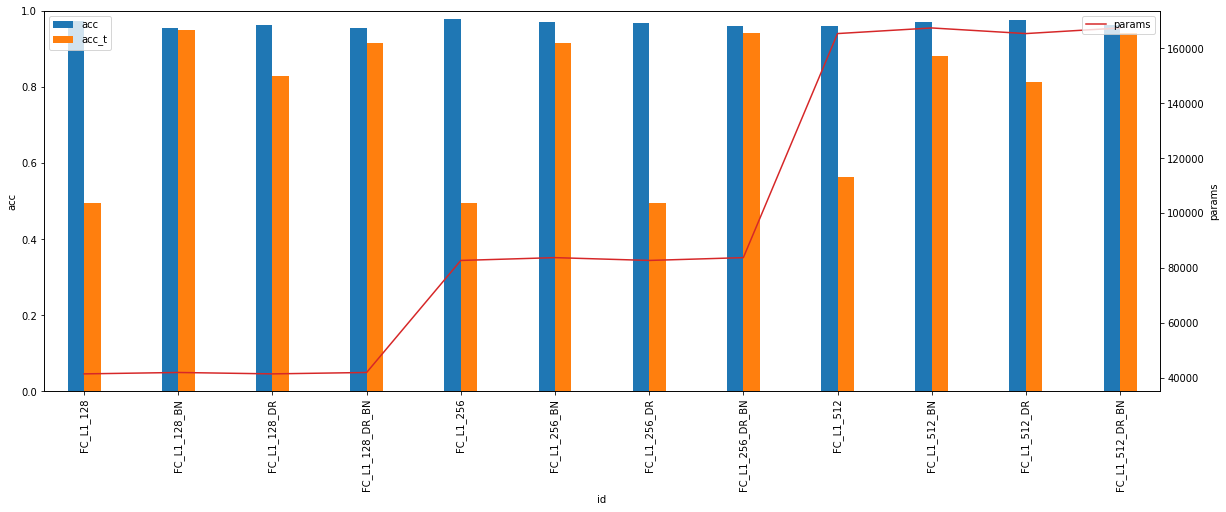
\includegraphics[width=1\textwidth]{thesistemplate/fig/fc_1layer_plot.png}
    \caption{One layer fully connected structure test, number of parameters in red line, number of nodes varied, while testing Dropout and BN. (Columns are: acc - accuracy on the test set, acc\_t - prediction accuracy on a custom speech recording from the mic used in the implementation.) }
    \label{fig:FC_1layer}
  \end{center}
\end{figure}

\subsubsection{Test with two linear layers}

The second experiment with FCN will focus on minimizing the number of parameters by adding another additional layer to a narrower first layer, hoping to maintain model generalizability even with smaller memory needs. The models consist of 128-32, 256-32, 64-16 node structures. As before the effect of Batch Normalization and Dropout was tested on every architectural choice.

The test results are reported at \autoref{fig:FC_2layer}. Similar to the first experiment the combination of both BN and DR lead to the highest accuracy most stable and reproducible results among the test cases. The lack of DR caused model overfitting in most cases, and the effect is visible when it was tested with the custom voice recording. And as the two rightmost models on the figure demonstrate, high-performing models can be trained even using as low as 20 thousand parameters with a carefully chosen architecture.

\begin{figure}[ht!]
  \begin{center}
    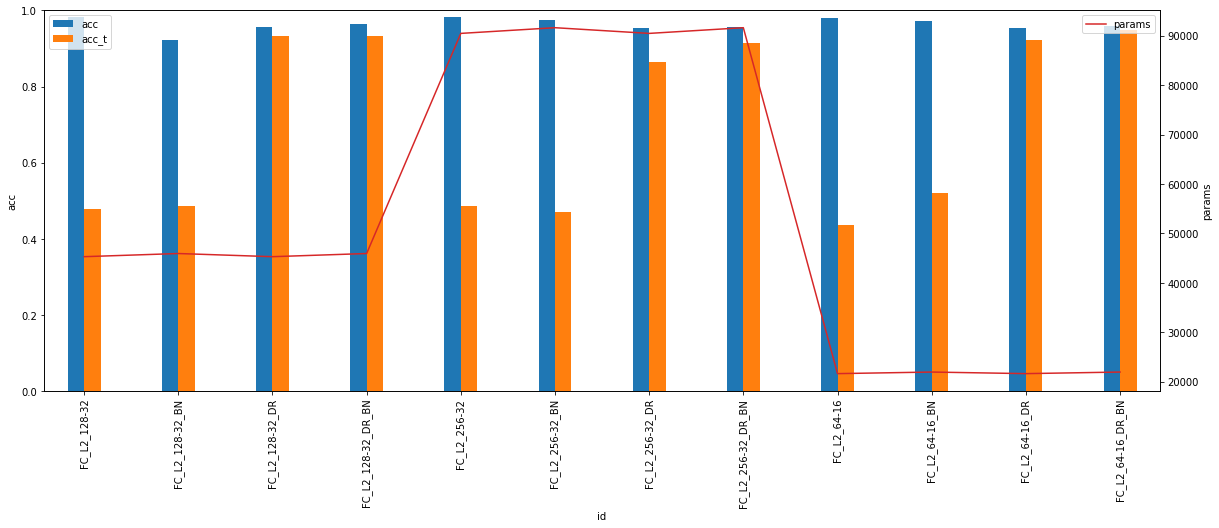
\includegraphics[width=1\textwidth]{thesistemplate/fig/test_fc_2lay_plot.png}
    \caption{Two layers of fully connected layer structure test, number of parameters in red line, number of nodes varied, effect of Dropout and BN. (Columns are: acc - accuracy on the test set, acc\_t - prediction accuracy on a custom speech recording from the mic used in the implementation.)}
    \label{fig:FC_2layer}
  \end{center}
\end{figure}

\subsubsection{Test with different dropout values}

In the last FCN based grid search training, the effect of different dropout rates (0, 0.25, 0.5) was tested with the combination of BN layers. Zero dropout rate means no dropout or identity function from an implementation point of view.

The test result reported at \autoref{fig:FC_2layer_small}. Models without dropout lead to overfitting and selecting smaller values such as 0.25 also does not help to reduce the effect on the second test set. However 50\% dropout rate have been proven to be sufficient for mitigating the model limitations and enabled good response on both test sets.

\begin{figure}[ht!]
  \begin{center}
    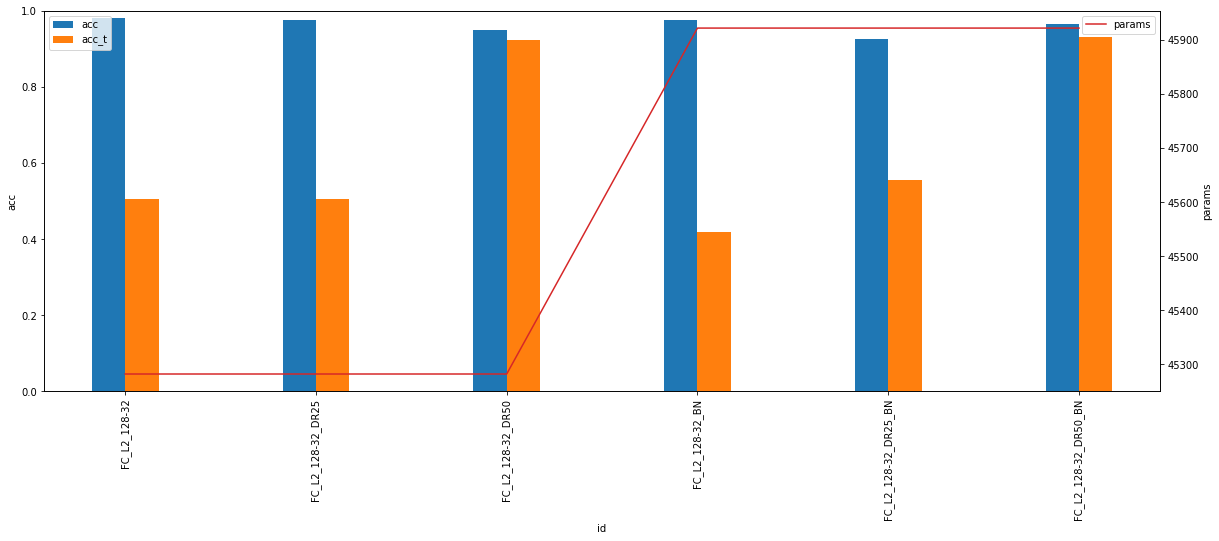
\includegraphics[width=1\textwidth]{thesistemplate/fig/test_fc_2lay_smalll_plot.png}
    \caption{The effect of different Dropout values (0, 0.25, 0.5) and Batch Normalization combined for the selected two layer Fully connected network.  (Columns are: acc - accuracy on the test set, acc\_t - prediction accuracy on a custom speech recording from the mic used in the implementation.)}
    \label{fig:FC_2layer_small}
  \end{center}
\end{figure}

\newpage
\subsection{Convolutional Neural Network experiments}

Constructing Convolutional Neural Networks applied the same principles as described in the previous FCN experimentation section. The architectural model schema is summarised in \autoref{fig:CNN_structure}. The three main parts are the Feature extractor the Classifier and the Head of the network. The feature extractor module consists of 2D Convolution, Batch Normalization, RelU Activation, and Max pooling. The position of the BN layer is between the convolution and the activation function as it was in the FCN networks and the BN paper \cite{ioffe2015batch}. The 2D Max pooling layer downsamples the input by a factor of two, by selecting the maximal value in each two-by-two pool frame size. Multiple feature extractors can be stacked after each other, and after that, a fully connected layer based Classifier comes. The Classifier can be configured to have multiple linear layers with arbitrary width and using or not the Dropout layer after the ReLU activation. The Dropout rate is kept to 50\% when it is used. Batch Normalization layers can be switched on and off in the Feature extractors by a parameter similarly. The Head module consists only of a linear layer as in the FCN case outputting probability values for each class.

\vspace{100px}

\begin{figure}[h!]
  \begin{center}
    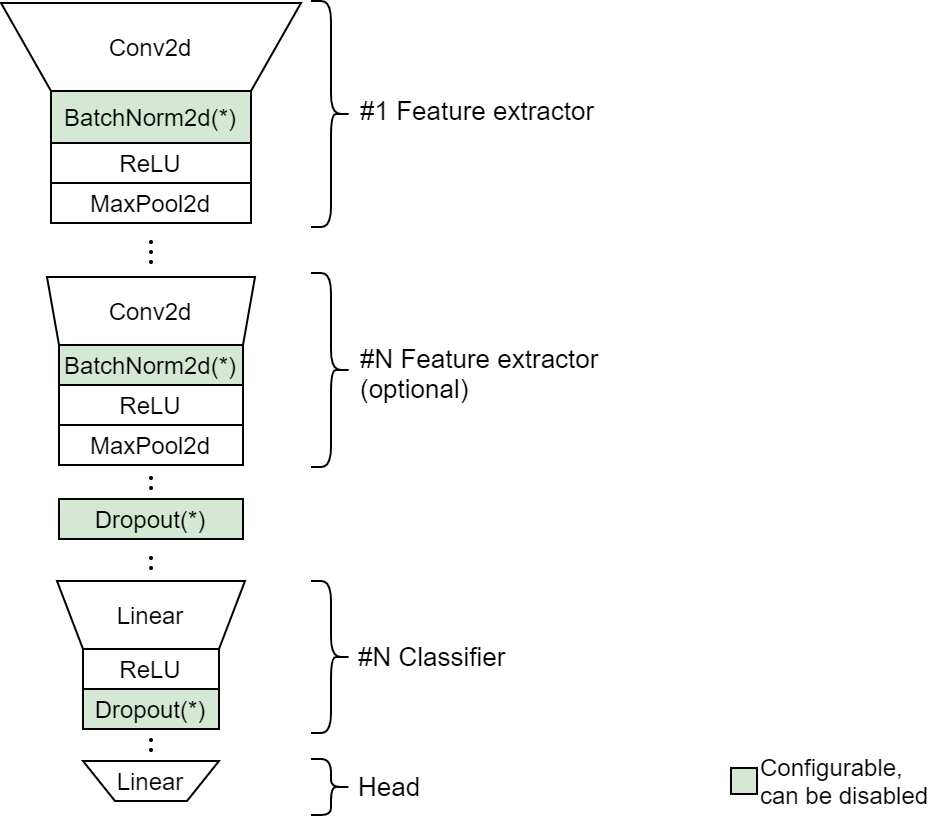
\includegraphics[width=0.7\textwidth]{thesistemplate/images/nn_layer_st_cnn.png}
    \caption{Flexible CNN model architecture, the number of Feature extractor and Classifier blocks can be altered, Batch Normalization and Dropout layers can be turned off.}
    \label{fig:CNN_structure}
  \end{center}
\end{figure}

CNN saved models follow a predefined naming convention to ease the archiving and logging process:

\begin{equation*}
CNN\_L\{layers\}\_K\{kernel\}\_F\{filters\}\_\{fc\_layers\}\_\{DR\}\_\{BN\}
\end{equation*}

\begin{table}[h!]
\begin{tabular}{l|l}
\textbf{Label}      & \textbf{Description}  \\
\hline
$layers$     & Number of Convolutional layers (Feature extractors) \\
$kernel$     & Size of the 2D convolution kernel \\
$filters$    & Number of filters learned in each Conv layer     \\
$fc\_layers$ & Structure of linear classifier, multilayer allowed \\
$DR$         & Dropout applied           \\
$BN$         & Batch Normalization applied           
\end{tabular}
\caption{CNN model naming convention.}
\end{table}

\begin{table}[h]
\centering
\begin{tabular}{lllr}
\hline
\textbf{Layer} & \textbf{Type}  & \textbf{Params} & \textbf{Output shape} \\
\hline
0     & Conv2D                      & 80     & (1, 18, 14, 8) \\
1     & BatchNormalization        & 32     & (1, 18, 14, 8) \\
2     & Activation (ReLU)           & 0      & (1, 18, 14, 8) \\
3     & MaxPooling                  & 0      & (1, 9, 7, 8)   \\
4     & Dropout                     & 0      & (1, 9, 7, 8)   \\
5     & Conv2D                      & 584    & (1, 7, 5, 8)   \\
6     & BatchNormalization        & 32     & (1, 7, 5, 8)   \\
7     & Activation (ReLU)           & 0      & (1, 7, 5, 8)   \\
8     & MaxPooling                  & 0      & (1, 3, 2, 8)   \\
9     & Dropout                     & 0      & (1, 3, 2, 8)   \\
10    & Flatten                     & 0      & (1, 48)        \\
11    & Linear                      & 6272   & (1, 128)       \\
12    & Dropout                     & 0      & (1, 128)       \\
13    & Linear                      & 4128   & (1, 32)        \\
14    & Dropout                     & 0      & (1, 32)        \\
15    & Linear                      & 66     & (1, 2)        \\ 
\hline
% Total params: 45922
\end{tabular}
\caption{Layer structure and number of parameters per layer for a two layer CNN with dropout and batch normalization, 8 filters, kernel size of 3$\times$3 classifier shape [128, 32] (CNN\_L2\_K3\_F8\_128-32\_DR\_BN). }
\end{table}




\subsubsection{Test for number of filters, filter size}


In the first test, visible on \autoref{fig:CNN_1layer}, the classifier shape was kept at constant 64 nodes, while the number of filters was varied in four different levels 2, 4, 8, and 16. Batch normalization and Dropout layers were altered in each case, providing a total of 16 combinations. Examining the accuracy results, overall, more filters usually resulted in better performance but there is no clear improvement by introducing significantly more filters to the model. Therefore a smaller structure K3\_F4, kernel size of 3$\times$3, and 4 learned filters are selected for further investigation.

\begin{figure}[ht!]
  \begin{center}
    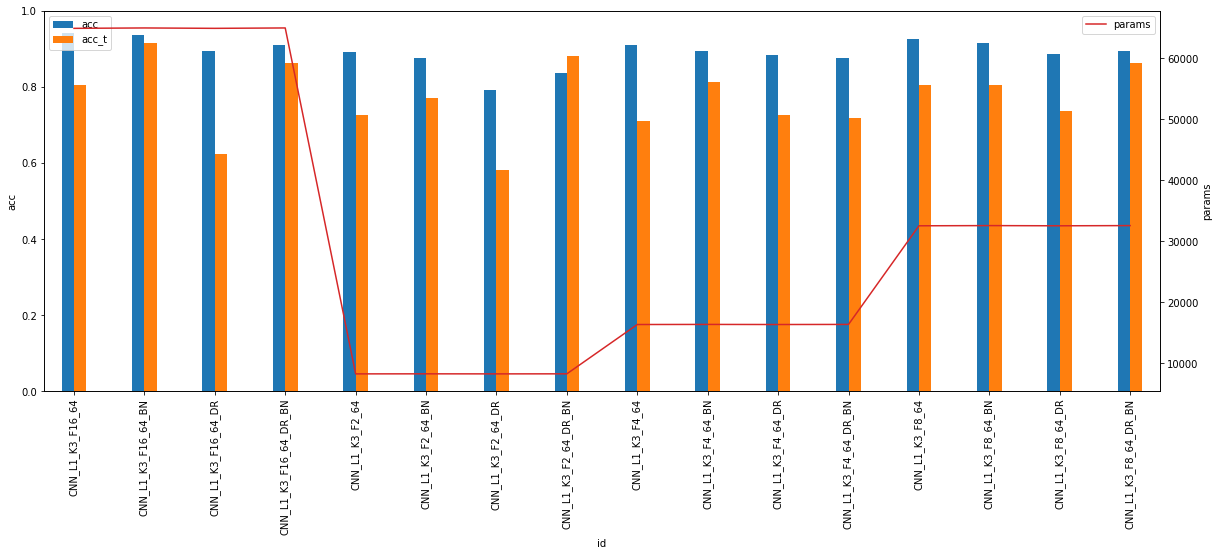
\includegraphics[width=1\textwidth]{thesistemplate/fig/test_cnn_1lay_plot.png}
    \caption{Number of filters does not really improve the accuracy, although it has a great impact in the total number of parameters. Usage of Batch Normalization and Dropout layers does not show significant improvements in this test. (Columns are: acc - accuracy on the test set, acc\_t - prediction accuracy on a custom speech recording from the mic used in the implementation.)}
    \label{fig:CNN_1layer}
  \end{center}
\end{figure}


\subsubsection{Test for one layer classifier with different width}

For the second experiment, we have varied the classifier size while keeping the feature extractor with kernel size 3$\times$3 and 4 filters. The accuracy results are reported at \autoref{fig:CNN_1lclassf}. Versions with dropout performed lower than the competition on average and using BN exclusively produced the best results. 

\begin{figure}[h!]
  \begin{center}
    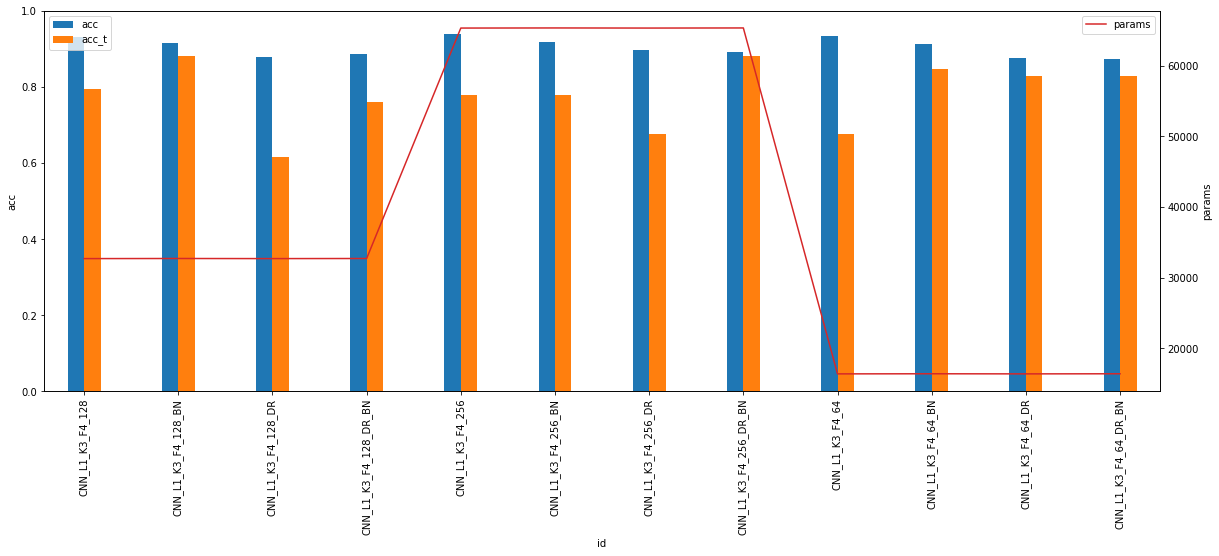
\includegraphics[width=1\textwidth]{thesistemplate/fig/test_cnn_clss_plot.png}
    \caption{One layer classifier different node sizes, BN, DR. (Columns are: acc - accuracy on the test set, acc\_t - prediction accuracy on a custom speech recording from the mic used in the implementation.)}
    \label{fig:CNN_1lclassf}
  \end{center}
\end{figure}


\subsubsection{Test for two layer classifier with different width}

In the last test, the effect of an additional fully connected layer in the classifier will be examined. Batch normalization is used without dropout, the only variation across the models is the classifier shape. Result are reported at \autoref{fig:CNN_classf}.

\begin{figure}[h!]
  \begin{center}
    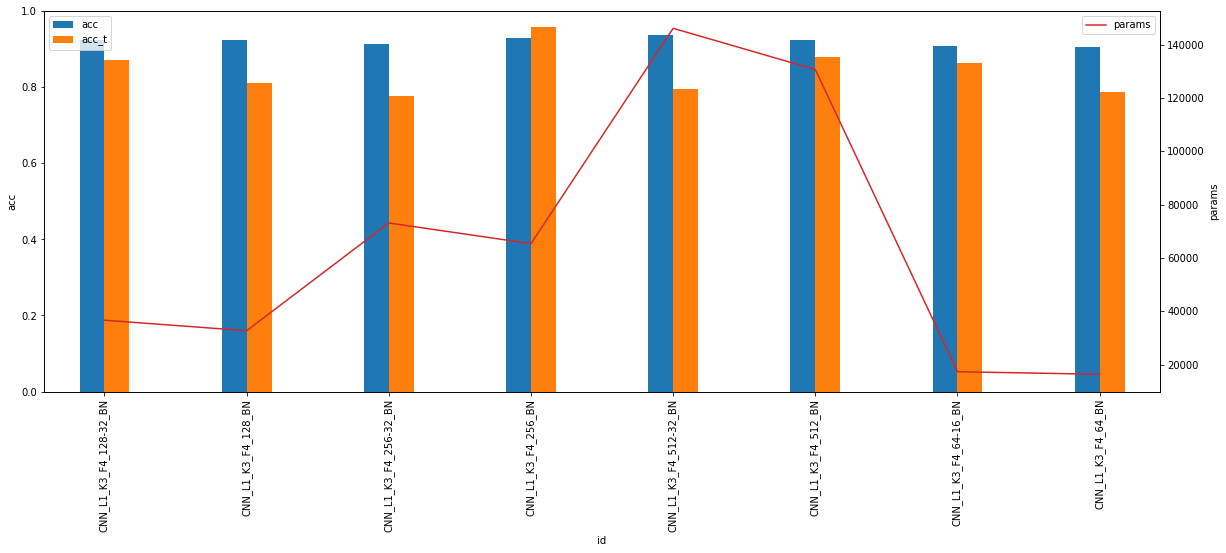
\includegraphics[width=1\textwidth]{thesistemplate/fig/test_cnn_clss2_plot.png}
    \caption{Experiment on one or two fully connected layer in the classifier while using Batch normalization. (Columns are: acc - accuracy on the test set, acc\_t - prediction accuracy on a custom speech recording from the mic used in the implementation.)}
    \label{fig:CNN_classf}
  \end{center}
\end{figure}




\section{Model selection for embedded implementation}

For the embedded study, four models were selected both from FCN and CNN training. During the selection, the aim was to represent distinctive elements of the search space with the highest accuracy values and least false-positive rates. All the four Fully-connected models utilize both Batch Normalization and Dropout layers, the main difference is in the number of layers and their width. Choosing only bigger networks might be a limiting factor computationally given the selected hardware components.

Among trained CNN models, all of the selected ones apply Batch Normalization and one also with Dropout. The main differentiator is in the classifier structure mainly, using one or two Fully-connected layers and smaller or bigger node sizes per layer.
\newline

% FCN models for embedded test (one layer small/large, two layers small/large):

% \begin{itemize}
%     \item[$-$] 1 layer, 128 nodes, DR, BN
%     \item[$-$] 1 layer, 256 nodes, DR, BN
%     \item[$-$] 2 layers, 64-16, DR, BN
%     \item[$-$] 2 layers, 128-32, DR, BN
% \end{itemize}


\begin{table}[h!]
\begin{tabular}{|l|l|l|l|}
\hline
\textbf{Name}                   &  \textbf{Node structure} & \textbf{Dropout} & \textbf{Batch Norm.} \\ \hline
FC\_L1\_128\_DR\_BN    & 128            & Yes     & Yes                 \\ \hline
FC\_L1\_256\_DR\_BN    & 256            & Yes     & Yes                 \\ \hline
FC\_L2\_64-16\_DR\_BN & 64-16          & Yes     & Yes                 \\ \hline
FC\_L2\_128-32\_DR\_BN  & 128-32         & Yes     & Yes                 \\ \hline
\end{tabular}
\caption{Selected Fully Connected Network model structures.}
\end{table}


\begin{table}[h!]
\begin{tabular}{|l|l|l|l|l|l|}
\hline
\textbf{Name}                        & \textbf{Kernel} &\textbf{Classifier}  & \textbf{Dropout} & \textbf{BN} \\ \hline
CNN\_L1\_K5\_F4\_64\_DR\_BN &  5$\times$5           & 64                        & Yes     & Yes                 \\ \hline
CNN\_L1\_K3\_F4\_256\_BN    &  3$\times$3           & 256                       & No      & Yes                 \\ \hline
CNN\_L1\_K3\_F4\_64-16\_BN  &  3$\times$3           & 64-16                     & No      & Yes                 \\ \hline
CNN\_L1\_K3\_F4\_128-32\_BN &  3$\times$3           & 128-32                    & No      & Yes                 \\ \hline
\end{tabular}
\caption{Selected Convolutional Neural Network model structures, BN - Batch Normalization.}
\end{table}

% CNN models for embedded test (one layer small/large, two layers small/large):
% \begin{itemize}
%     \item 1 layer, 64 nodes, DR, BN
%     \item 1 layer, 256 nodes, BN 
%     \item 1 layer, 64-16 nodes, BN
%     \item 1 layer, 128-32 nodes, BN
% \end{itemize}



% FCN:
% FC_L1_128_DR_BN  - test_fc_1lay
% FC_L1_256_DR_BN  - test_fc_1lay
% FC_L2_128-32_DR50_BN - test_fc_2lay_small
% FC_L2_64-16_DR_BN - test_fc2lay

% CNN
% CNN_L1_K5_F4_64_DR_BN - the one, (second working model)
% CNN_L1_K3_F4_256_BN   - test_cnn_clss
% CNN_L1_K3_F4_64-16_BN - test_cnn_clss2
% CNN_L1_K3_F4_128-32_BN - test_cnn_clss2













%----------------------------------------
%
% Alternative table for audio database


%\begin{table}[ht]
%\centering
%\begin{tabular}[t]{lr}
%\hline
%Type                        & duration\\
%\hline
%\textit{Occupied:}           & \\
%
%Librispeech dev             &  323:16\\
%QUT-Noise home-kitchen      &   33:09\\
%Open office recordings      &   10:00\\
%\hline
%Total:                      &  366:25\\
%\hline
%\\
%\textit{Empty:}              &       \\
%Meeting room recordings     &   43:00\\
%QUT-Noise car-window        &   44:35\\
%White noise                 &   15:00\\
%\hline
%Total:                      &  102:35\\
%\hline
%\end{tabular}
%\caption{Audio Database size}
%\end{table}%
 





% You have now stated your problem, and you are ready to do something
% about it!  \emph{How} are you going to do that? What methods do you
% use?  You also need to review existing literature to justify your
% choices, meaning that why you have chosen the method to be applied in
% your work.

% An example of a traditional LaTeX table
% ------------------------------------------------------------------
% A note on underfull/overfull table cells and tables:
% ------------------------------------------------------------------
% In professional typography, the width of the text in a page is always a lot
% less than the width of the page. If you are accustomed to the (too wide) text
% areas used in Microsoft Word's standard documents, the width of the text in
% this thesis layout may surprise you. However, text in a book needs wide
% margins. Narrow text is easier to read and looks nicer. Longer lines are 
% hard to read, because the start of the next line is harder to locate when
% moving from line to the next. 
% However, tables that are in the middle of the text often would require a wider
% area. By default, LaTeX will complain if you create too wide tables with
% ``overfull'' error messages, and the table will not be positioned properly
% (not centered). If at all possible, try to make the table narrow enough so
% that it fits to the same space as the text (total width = \textwidth).
% If you do need more space, you can either
% 1) ignore the LaTeX warnings 
% 2) use the textpos-package to manually position the table (read the package
%    documentation)
% 3) if you have the table as a PDF document (of correct size, A4), you can use
%    the pdfpages package to include the page. This overrides the margin
%    settings for this page and LaTeX will not complain.
% ------------------------------------------------------------------
% Another note:
% ------------------------------------------------------------------
% If your table fits to \textwidth, but the cells are so narrow that the text
% in p{..}-formatted cells does not flow nicely (you get underfull warnings 
% because LaTeX tries to justify the text in the cells) you can manually set
% the text to unjustified by using the \raggedright command for each cell 
% that you do not want to be justified (see the example below). \raggedleft 
% is also possible, of course...
% ------------------------------------------------------------------
% If you need to have linefeeds (\\) inside a cell, you must create a new
% paragraph-formatting environment inside the cell. Most common ones are 
% the minipage-environment and the \parbox command (see LaTeX documentation
% for details; or just google for ``LaTeX minipage'' and ``LaTeX parbox'').

 
\chapter{Implementation}
\label{chapter:implementation}

% \emph{[- Embedded -  Trained Model deployment to embedded microcontroller, quantization, STM32 platform specifics, audio handling, NN model options]}
% \bigskip

After selecting the best performing models in this chapter we are aiming to run the inference with real-time data collection on an embedded microcontroller platform and finally assemble a real-time multisensory room occupancy detector, by interfacing with a PIR sensor and merge the predictions.

\section{Embedded hardware platform}

Choosing a specific company or product line for embedded software development has to be planned with great care. Chip manufacturers and prototype makers create their unique solutions and development environments making it exceptionally hard to switch platforms within the industry with the additional steep learning curve for application development. Our task involves audio processing, feature extraction, and machine learning inference just to mention the most computationally demanding ones. Moreover, trained models usually require a relatively large amount of memory for storing the weights and biases, therefore various techniques are developed to reduce the memory footprint by transferring the model parameters to lower resolution fixed-point numbers like in quantization or compress the model (weight sharing algorithm, K-means clustering, only for fully connected layers..).


Hardware requirements:
\begin{itemize}
    \item Deep Learning requirements: increased memory for model parameters (64KB+), FPU, DSP instructions 
    \item Digital audio processing requirements:  peripheral to memory DMA, I\textsuperscript{2}S bus, 16k sample rate option
\end{itemize}

\section{STMicroelectronics}

Based on the criteria described above the firm STMicroelectronics was chosen due to its wide portfolio of microprocessors and development boards in our target range and software support tools for fast prototyping such as project generation by CubeMX or machine learning model conversion by X-CUBE-AI. Among their development boards, we aimed to find a cost-efficient option with DSP and FPU with the necessary communication interfaces for a digital MEMS microphone. 


Software tools used for initial project generation:
\begin{itemize}
  \item  \textbf{STM32CubeMX} is an official graphical tool for microcontroller and interface peripheral configuration with C code generation for the selected environment. As a final result, the user can focus more on the application development given that the peripheral initialization and library compatibility issues are already resolved automatically. The tool enables the user to select the desired microcontroller or development board and configure the GPIO and clock settings in an assisted manner, while the pinout-conflict solver aims to spot when a pin is used for multiple purposes and suggest alternative options. Moreover, the software functionality can be extended with various expansion packages too, in our project the only the X-CUBE-AI add-on is used.
  \item  \textbf{X-CUBE-AI} is a STM32CubeMX Expansion Package for automatic conversion of pre-trained Deep Neural Networks and optimized library generation for AI projects. The tool expects a saved Tensorflow Lite, Keras, or ONNX model to convert it to an efficient C library for inference purposes only. It supports 8-bit model quantization for processors without FPU and model compression for fully connected layers only.
 \item  \textbf{STM32CubeIDE}: The STM32CubeIDE is ST's own Eclipse-based multi-OS supported Integrated Development Environment (IDE) for embedded microcontrollers. Rich programming and debugging features make it a truly versatile tool.
\end{itemize}  

  
Software libraries:
\begin{itemize}
  \item \textbf{CMSIS}: Cortex Microcontroller Software Interface Standard, developed by ARM, provides a generic API for all Arm Cortex processors, simplifying software reuse and maximizing the computational performance of chips. Functions from their DSP module are utilized for audio signal processing in this project while the CMSIS-NN module is used by the X-CUBE-AI tool for generating efficient neural network instances for inference. Arm-based research \cite{lai2018cmsisnn} shows that CMSIS-NN based kernels can demonstrate a significant amount of increase (2.5x to 5x) in throughput and energy efficiency compared to traditional approaches.
  % https://arxiv.org/pdf/1801.06601.pdf
  
  \item  \textbf{STM32 AI Audio Preprocessing library} is a generic C library for audio frequency domain analysis and feature extraction, such as spectrogram, mel-scaled spectrogram computation, and Mel-frequency cepstral coefficient (MFCC) extraction. Uses the CMSIS DSP library for runtime optimization.
  
  \item  \textbf{HAL library} is an acronym for Hardware Abstraction Layer. STM32 provides a generic, high-level, feature-oriented Application Programming Interface (API) for development, allowing portability across the company's various microcontroller options. The HAL library hides the complexity of the selected MCU and peripherals, therefore helps the engineer to focus on application-specific challenges.
  \item  \textbf{BSP drivers} or Board Support Package is a set of functions ready-made for the selected board based on the HAL drivers. The goal is to speed up the prototyping phase by providing the necessary configuration and interfacing endpoints for components and peripherals fixed on the development board. Examples contain LEDs user buttons, or other board-specific peripherals such as LCD, Audio, or Touchscreen. Configurations may be overwritten by the user if certain settings are not wanted, but it is only recommended after careful consideration since the hardware connections might cause undesired behavior.

\end{itemize}

%STM32 code sources
% https://www.st.com/content/st_com/en/ecosystems/stm32-ann.html
% https://www.st.com/en/embedded-software/fp-ai-sensing1.html
% https://github.com/anderslanders/stm32-smart-headphones

\subsection{STM32 Nucleo-64 board}

The selected prototyping board for testing is the Nucleo-F401RE. It is one of the top-end models of the Nucleo-64 high-performance product line with an integrated ST-LINK debugger, programmer, and virtual COM port, allowing the user to start the development easily by connecting it to the computer with a single USB cable. 



\begin{table}[h!]
\begin{tabular}{|l|l|}
\hline
\textbf{Feature}                  & \textbf{STM32F401RE}             \\ \hline
Clock frequency                   & 84 MHz                           \\ \hline
Flash                             & 512 KB                           \\ \hline
SRAM                              & 96 KB                            \\ \hline
FPU                               & Available                        \\ \hline
Cache                             & None                             \\ \hline
Adaptive Real-time Accelerator(ART)    & Available                   \\ \hline
Timers                            & 11 Timers                        \\ \hline
DMA controllers                   & 2 DMAs                        \\ \hline
UART                              & 3 USARTs                         \\ \hline
Serial Peripheral Interface (SPI) & 4 SPIs (2 I\textsuperscript{2}Ss can be configured) \\ \hline
USB Interface                     & 1 USB 2.0                        \\ \hline
\end{tabular}

\caption{STM32 microcontroller specification summary.}
\end{table}


\subsection{Peripherals}

In the next sections, the selected hardware peripherals and their interfacing options with the selected microcontroller will be elaborated. Most importantly the audio and the PIR sensor properties and applicability for the test use case and the necessary Digital Signal Processing steps as a prerequisite for matching the input for the machine learning inference.


\subsubsection{Audio sensor}
\label{subsub:Aud_sensor}

The chosen audio sensor for the embedded implementation is the Adafruit I\textsuperscript{2}S MEMS Microphone Breakout board with a Knowles SPH0645LM4H MEMS Digital Microphone. The advantage of using an I\textsuperscript{2}S digital microphone over an analog version, is the compactness of the solution, quick prototyping results, and the direct connection with the MCU without an external audio codec. On the other hand, an inherent disadvantage of such compact boards that it does not give any room for customization, additional analog filtering or just to access the raw analog microphone signal is impossible.


\begin{table}[h!]
\centering
\begin{adjustbox}{max width=1\textwidth}
\begin{tabular}{|l|c|c|c|c|c|}
\hline
\textbf{Parameter}             & \textbf{Conditions}                    & \textbf{Min.}        & \textbf{Typ.}        & \textbf{Max}        & \textbf{Units}      \\ \hline
Directivity           &                              & \multicolumn{4}{c|}{Omnidirectional}            \\ \hline
Polarity              & Increasing sound pressure    & \multicolumn{4}{c|}{Output Magn. Increases} \\ \hline
DC Offset             & Fullscale $= \pm $  100    & -          & 5          & -         & \%        \\ \hline
Sensitivity           & 94 dB SPL @ 1kHz             & -27        & -26        & -25       & dBFS      \\ \hline
Signal to Noise Ratio & 94 dB SPL @ 1kHz, A-weighted & -          & 65         & -         & dB(A)     \\ \hline
Power-up Time         & V\textsubscript{DD} $\geq$ V(min) & -          & -          & 50        & ms        \\ \hline
\end{tabular}

\end{adjustbox}

\caption{Knowles SPH0645LM4H microphone specification summary \cite{knowles_mems}.}
\end{table}

The directionality of the microphone indicates the signal sensitivity change with respect to the arrival of the sound. The selected MEMS microphone is omnidirectional by design, so there is no or very little change in the measurements when the relative angle of the sound source is altered. Flat frequency response in the 100 to 8 kHz range.

The schematic diagram of an I2S MEMS microphone is shown in \autoref{fig:mems_schematic}. The sensor acts as a silicon capacitor while the ASIC Application Specific Integrated Circuit converts the analog signal first to digital by amplification and sigma-delta conversion PDM to PCM and finally transfers the signal through the I2S bus.
%https://www.st.com/resource/en/application_note/dm00103199-tutorial-for-mems-microphones-stmicroelectronics.pdf
\begin{figure}[h!]
  \begin{center}
    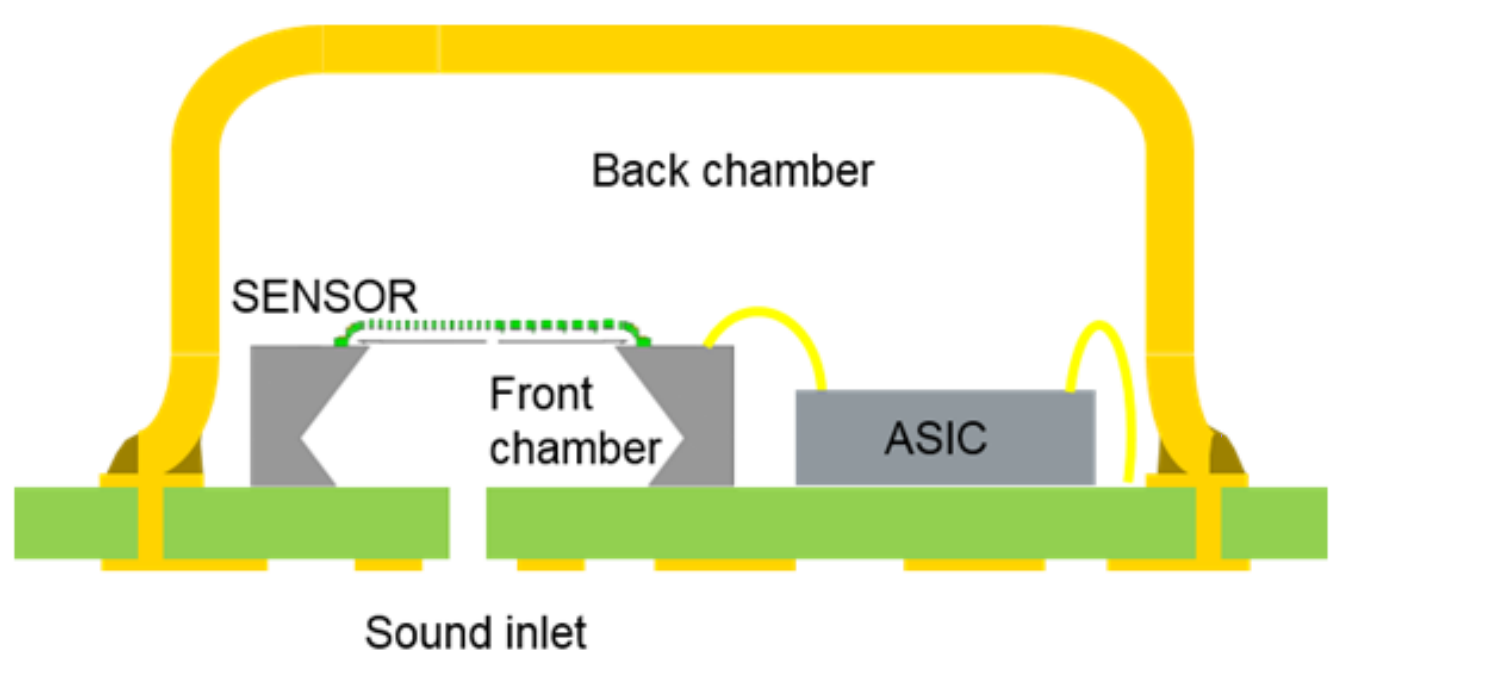
\includegraphics[width=0.5\textwidth]{thesistemplate/images/mems_schematic.png}
    \caption{MEMS Microphone schematic diagram with integrated ASIC \cite{mems_tutor}.}
    \label{fig:mems_schematic}
  \end{center}
\end{figure}



\subsubsection{I\textsuperscript{2}S communication interface}

The Inter-IC Sound (I\textsuperscript{2}S) bus protocol was developed by Philips in the late 1980s, as a constructive attempt for standardized communication of digital audio between electronic components. To minimize the number of pins required while keeping the protocol simple to decode, it uses a 3 lines serial bus: SD the Serial Data channel, WS or Word Select line, and SCK the Serial Clock line. In the data transmission, it is the master's task to generate the SCK and WS signals, in our case the STM32 microcontroller. The WS line indicates which channel (left or right) is being transmitted on the Data line, and it is changed one clock period before the MSB (Most Significant Bit).

The data provided by the I\textsuperscript{2}S slave microphone is 24-bit two's compliment MSB first, in Pulse Code Modulated (PCM) format. Since the sensor data precision is 18 bit only, the last 6 bits are always zeros and after the 24 bit sent the Data bus is changed to a high impedance(tri-state) state for the remaining part of the 32-bit data frame.

The selected sample rate is 16 kHz, similarly to most of the audio recordings used for training, even if higher sampling frequency options were supported, the additional higher resolution recordings have not been proven significantly beneficial during the testing, moreover it imposes considerable computational overhead.


\begin{figure}[h!]
  \begin{center}
    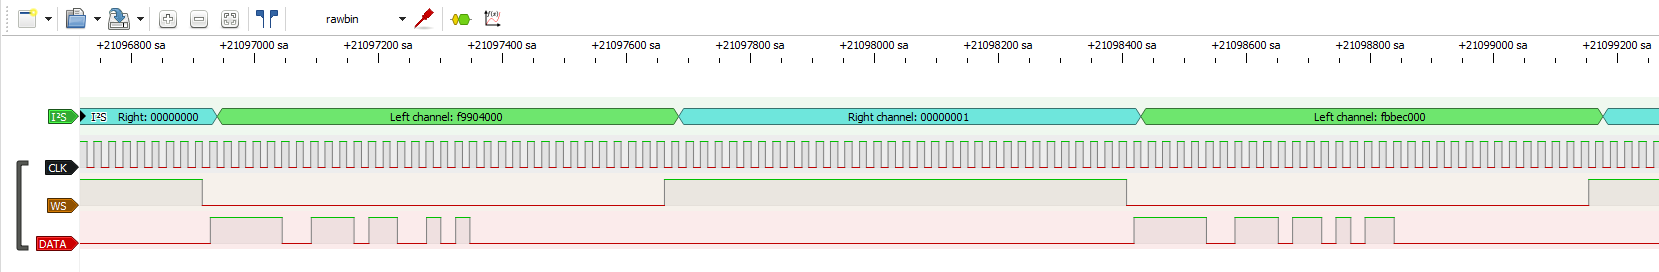
\includegraphics[width=1\textwidth]{thesistemplate/images/i2s_signal2.png}
    \caption{I\textsuperscript{2}S communication with Logic Analyzer and Protocol Decoder.}
    \label{fig:i2s_comm_prot_meas}
  \end{center}
\end{figure}

\begin{figure}[h!]
  \begin{center}
    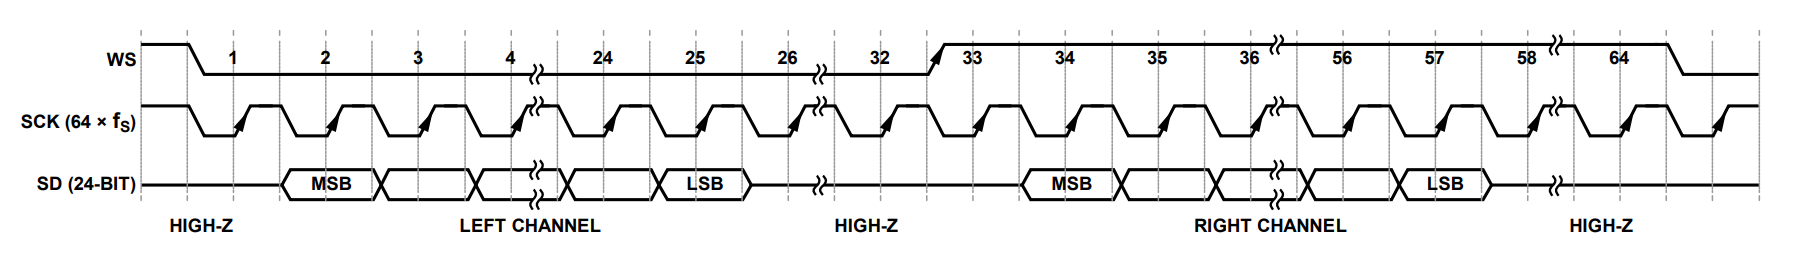
\includegraphics[width=1\textwidth]{thesistemplate/images/i2s_signal_datasheet.png}
    \caption{I\textsuperscript{2}S communication protocol example.}
    \label{fig:i2s_comm_prot}
  \end{center}
\end{figure}
% https://invensense.tdk.com/wp-content/uploads/2015/02/INMP441.pdf

% I2S specification, but we might need a better one for reference + the STM32 datasheet
% https://www.sparkfun.com/datasheets/BreakoutBoards/I2SBUS.pdf
% https://www.st.com/resource/en/reference_manual/dm00096844-stm32f401xbc-and-stm32f401xde-advanced-armbased-32bit-mcus-stmicroelectronics.pdf



\subsubsection{Audio DC component blocking filter}
\label{subsub:dc_blocking}

As elaborated in the datasheet of the chosen microphone MEMS microphone devices have a typical DC offset about 5 \% of the full range. Fortunately, the offset remains constant in the time frame of examination, therefore it is relatively easy to remove it without much distortion in the signal.

In the digital signal processing domain, various solutions exist for mitigating this problem. Keep tracking of a moving average and subtracting it from the audio stream is a straightforward approach and most resembles the process needed in the bias removal step of the data analysis. Based on research literature, it is a common practice to utilize a differentiator-integrator module to eliminate the DC component of a signal.

Exploiting the DSP capabilities of the STM microcontroller there is a simple and efficient way to implement a high-pass filter using the CMSIS DSP library. The task is to define the IIR filter parameters which fulfill the requirements. Second-order biquad filters are can be configured to execute the filtering in real-time on the audio stream. An example visualization of such filter is reported at \autoref{fig:biquad}.

In the discrete complex frequency domain, a DC blocking filter transfer function can be constructed with one pole and one zero and defined as:

\begin{equation}
   H(z) = \frac{Y(z)}{X(z)} = \frac{1-z^{-1}}{1-pz^{-1}} ,
\end{equation}

where the coefficient $p$ determines the cut off frequency and the system responsiveness. After cross multiplication, we get:

\begin{equation}
    Y(z)(1-pz^{-1}) = X(z)(1-z^{-1})  
\end{equation}


After removing the parentheses we can transform the equation to the discrete-time domain using common Z-transform pairs:

\begin{equation}
    y[n] - p\, y[n-1] = x[n] - x[n-1]
\end{equation}


\begin{equation}
    y[n]  = x[n] - x[n-1] + p\, y[n-1]
\end{equation}

Which now can be easily realized with a Single Biquad filter (IIR) efficiently, provided by the MCU hardware. The output of the filter in the discrete-time domain is given by the following equation:

\begin{equation}
y[n] = b_0 \, x[n] + b_1\,  x[n-1] + b_2\,  x[n-2] + a_1\,  y[n-1] + a_2\,  y[n-2]
\end{equation}

\begin{figure}[h!]
  \begin{center}
    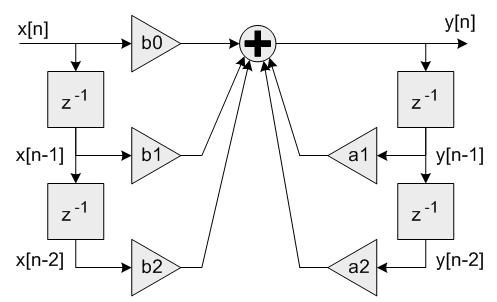
\includegraphics[width=0.5\textwidth]{thesistemplate/images/Biquad.png}
    \caption{Single Biquad filter provided by the CMSIS library.}
    \label{fig:biquad}
  \end{center}
\end{figure}

And finally from the last two equations the parameters can be inferred:


\begin{equation}
\label{eq:a_zero}
\begin{aligned}
a_1=p, b_0 = 1 \\
 a_2=0, b_1 = -1\\
b_2 = 0
\end{aligned}
\end{equation}

Recommendation for $p$ is provided by the microphone manufacturer for fixed and floating-point implementations \cite{knowles_dc_filter}. 

\begin{equation*}
    p = 1-2^{-12} \approx 0.99975586
\end{equation*}

% \begin{itemize}
%     \item TODO: Plot filter Bode diagram
% \end{itemize}

The effect of the filter on a short audio signal sample is demonstrated at \autoref{fig:dc_blocking_test}. Note that the simulation is plotted after the startup transition interval, in steady-state. No other additional filtering were added to the microphone signal. The DC-filtered signal will provide the basis for further signal processing steps related to feature extraction in frequency domain.

\begin{figure}[h!]
  \begin{center}
    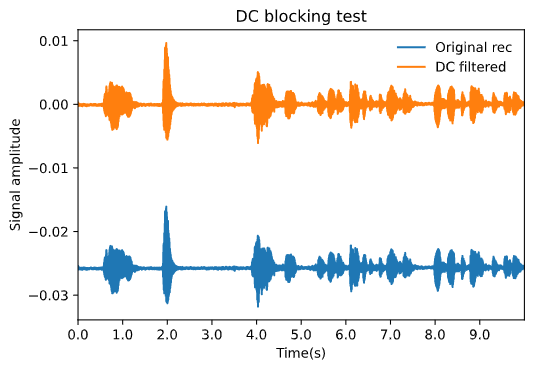
\includegraphics[width=0.7\textwidth]{thesistemplate/fig/dc_blocking.png}
    \caption{Testing the DC blocking filter functionality.}
    \label{fig:dc_blocking_test}
  \end{center}
\end{figure}



\subsubsection{PIR sensor}

The selection of a highly reliable and cost-effective motion sensor is also a key to the success of the project. After careful consideration of market alternatives, we have settled with the product portfolio provided by Panasonic. Their offering covers a wide variety of devices for different environments and signal output options. To simplify the development and match our design needs we have selected a digital PIR sensor (Panasonic EKMC167111) with a typical installation height of 3m with a relatively wide field of view (110$^{\circ}$) and 32 detection zones. The motion detection sensor will provide a logical high voltage level on the OUT pin in every situation when more than 4 $^{\circ}$C temperature difference is detected in two of the detection areas.

\begin{table}[h!]
\centering
\begin{tabular}{|l|l|}
\hline
\textbf{Parameter}                  & \textbf{Panasonic PIR EKMC}\\ \hline
Detection distance                  & up to 5 m                \\ \hline
Typical ceiling installation height & 3 m                      \\ \hline
Field of view                       & 110$^{\circ}$ $\times$ 110$^{\circ}$ \\ \hline
Detection zones                     & 32                       \\ \hline
Output type                         & Digital                  \\ \hline
Standby current consumption         & 170 \textmu A                 \\ \hline
\end{tabular}
\caption{Panasonic Digital PIR sensor specification summary \cite{papir_dsheet}.}
\end{table}

A cutaway diagram of a sample motion detector manufactured by Panasonic is shown at \autoref{fig:papir}. Unlike other companies on the market, their solutions include a tiny ASIC (Application Specific Integrated Circuit) inside the sensor case too, all integrated into a TO-5 sized metal can. The metal cover isolates the highly sensitive electronic components from electromagnetic fields caused by wireless devices, effectively preventing false alarms caused by interference. In the digital PIR sensors the ASIC performs differential signal amplification with an Operational amplifier coming from the analog Pyroelectric elements and implements a simple thresholding operation with a Comparator circuit. The output is a simple logical high or low voltage level based on the Comparator output. The spatial position and the number of detection zones are carefully controlled by the custom-designed Fresnel lens array on top of the sensing elements.

\begin{figure}[h!]
  \begin{center}
    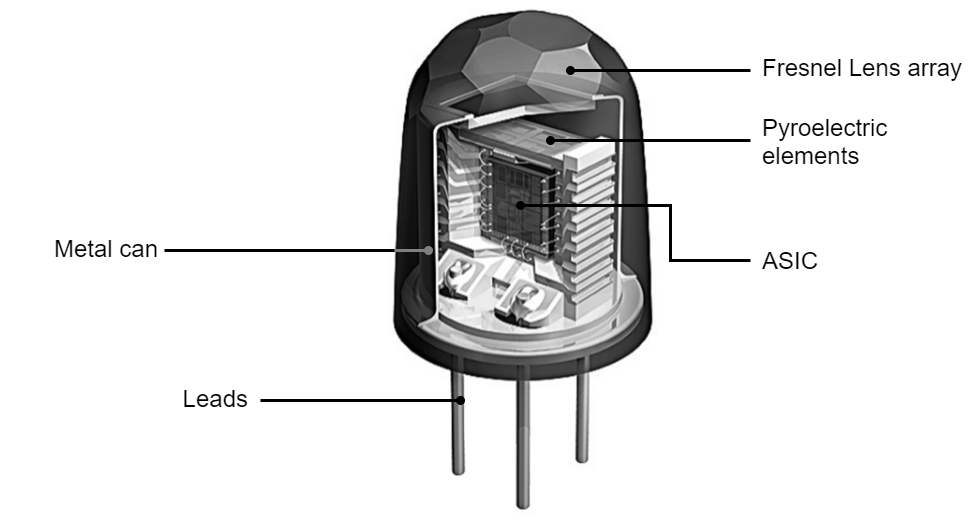
\includegraphics[width=0.9\textwidth]{thesistemplate/images/pir_cutaway.png}
    \caption{Panasonic PIR sensor cutaway diagram, adapted from the sensor datasheet \cite{papir_dsheet}.}
    \label{fig:papir}
  \end{center}
\end{figure}

% software
\section{Embedded Machine Learning model conversion and performance tests}

After when we found a feasible model structure that can also fulfill the requirements of the embedded platform we can convert the trained model to the MCU and run the inference to get real-time predictions. Dropout is removed during conversion by the STM32 provided X-Cube-AI tool, while conv and pool layers are fused by the tool for runtime-optimization reasons.


The handpicked best models from the previous chapter are tested by the following four performance measures:
\begin{itemize}
    \item[$-$] RAM memory requirements
    \item[$-$] Flash memory requirements
    \item[$-$] Execution time for inference
    \item[$-$] Complexity, MACC 
\end{itemize}

The performance tests serve also as a benchmark for the selected microcontroller platform to distinguish whether the available memory and computational power are sufficient to run a selected model inference in real-time. Additional resources need to be allocated to the audio feature extraction and other peripherals.

\subsection{RAM}

RAM is used only to store the intermediate (temporary) results during inference. The amount of space required for the application is excluded from the measurements. The same reserved memory block is used across different layers, reducing the size need. The RAM memory usage by layer can be examined for a selected network upon request.

\begin{figure}[h!]
  \begin{center}
    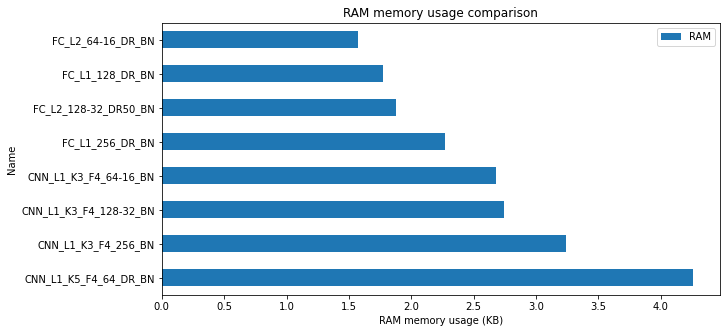
\includegraphics[width=1\textwidth]{thesistemplate/fig/ram_comp_emb.png}
    \caption{RAM memory requirements of the machine learning models tested.}
    \label{fig:ram_comp_emb}
  \end{center}
\end{figure}

Regarding the MCU limitations from the available 96 KB of RAM memory, even the largest one is just about 4.2 KB, consuming less than 5\% of the total memory space present.

\subsection{Flash}

The flash or ROM memory is used to store the weights and biases of the model. Additional space for the application was not included in the measurements. The model parameters and the compiled application code are written next to each other in the Flash memory space, but the reported values only representing the machine learning model memory needs.


\begin{figure}[h!]
  \begin{center}
    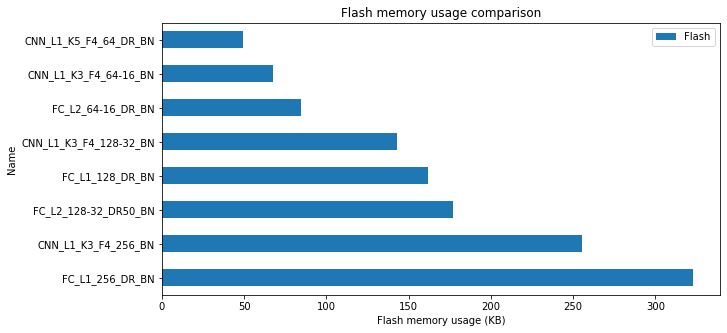
\includegraphics[width=1\textwidth]{thesistemplate/fig/flash_comp_emb.png}
    \caption{Flash memory requirements of the tested machine learning models tested.}
    \label{fig:flash_comp_emb}
  \end{center}
\end{figure}

Considering the total available flash space, 512 KB, larger models restrict the application by a large amount. The two largest models require 50\% and 65\% respectively, which might be a limiting factor for more complex problems.

\subsection{Inference time}

Inference time is measured as the total amount of time needed to propagate the input through the neural network and produce one output sequence.

\begin{figure}[h!]
  \begin{center}
    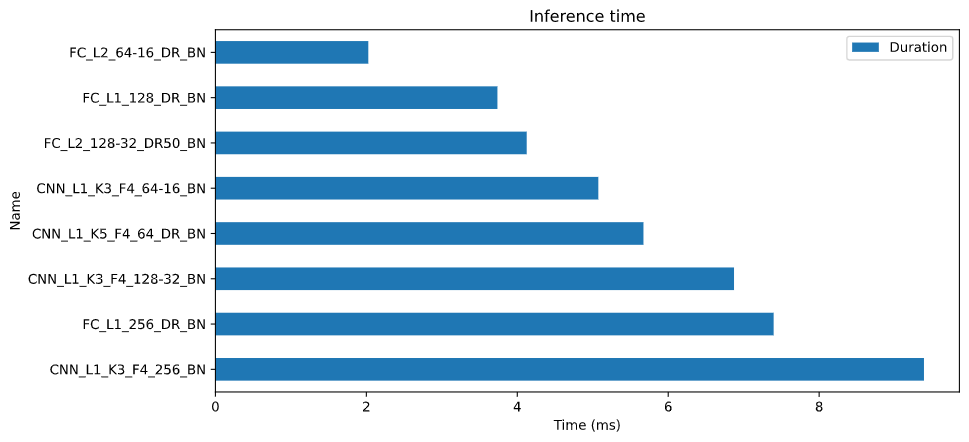
\includegraphics[width=1\textwidth]{thesistemplate/fig/inference_time.png}
    \caption{Inference time comparison for the machine learning models tested.}
    \label{fig:inference_time_comp_emb}
  \end{center}
\end{figure}

Examining the results depicted in \autoref{fig:inference_time_comp_emb} and running the microcontroller at 84 MHz, at its maximal speed, the inference process took less than 9 ms even in the most demanding scenario. As we will see in the following sections, this satisfies the real-time requirements for all of the selected models, since in the worst case one new column for the input needs to be computed in every 32 ms and about every 500 ms a new image will be constructed for inference.

\subsection{Complexity}

Complexity indicates the computational complexity of one inference process. It is common in embedded applications to approximate the complexity by the amount of Multiply And Accumulate (MACC) operations. The tests include an approximation of the activation functions and other general layers (Pooling, Batch Normalization) for the final estimations. 

On the selected M4 ARM chip each MACC operation takes is approximately 8 CPU cycles for FCN networks, while this value is slightly higher for CNN networks, around 12 in our test application. As it is visible on the results reported in \autoref{fig:complexity_comp_emb}, larger networks with more parameters generally require significantly more MACC operations, and the width of the fully connected layers are the most dominant influential factor.

\vspace{40px}

\begin{figure}[h!]
  \begin{center}
    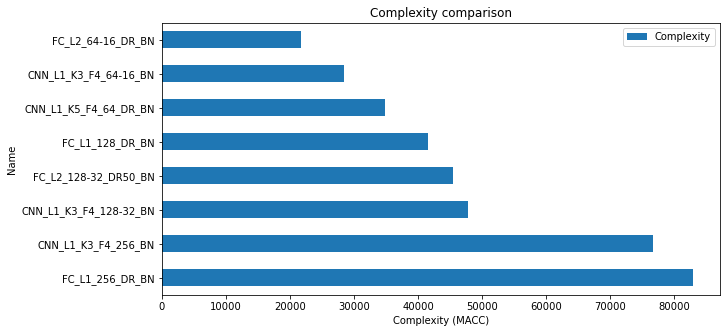
\includegraphics[width=1\textwidth]{thesistemplate/fig/complexity_comp_emb.png}
    \caption{Computational complexity comparison for the machine learning models tested.}
    \label{fig:complexity_comp_emb}
  \end{center}
\end{figure}


\section{Embedded AI process}

To benefit from the trained machine learning models on embedded we need to replicate the same data processing and feature extraction steps as in the PC version in python, but now in Embedded C, in a highly resource-constrained environment.

The data collection and preprocessing steps until the two-dimensional MFCC image construction are summarized in \autoref{fig:embedded_ai_proc}. To provide an instantaneous response to the final user the audio flow and the feature computation are continuous yielding one new occupancy prediction in each 500 ms.

The process starts with data fetching from the microphone. The audio sampling rate was kept at 16 kHz and 18-bit PCM samples were transferred through one of the I2S buses of the microcontroller in 32-bit frames. On the whole, the audio stream from one mic produces 62.5 KB/s of constant data flow, which if handled by the CPU, would have consumed most of its resources only just to move the data from peripheral to memory. Fortunately, the task can be outsourced to one of the two Direct Memory Access (DMA) controllers of the MCU, alleviating the need for CPU-based data movement. The DMA gets assigned to a fixed size of memory at the initialization step and during runtime, it keeps copying new samples to a circular buffer. The CPU will get notified through an interrupt request when the buffer is at half-full and full state, signaling the moment for the start of the signal processing tasks. By design, the size of the DMA input buffer is matching the number of samples needed to calculate one set of MFCC features, which is 512 samples, representing 32 ms of audio.

After when we have one set of 18 bit PCM coded audio first we convert it to 32-bit floating-point numbers, then we apply the IIR filter designed in section \ref{subsub:dc_blocking} for the DC offset removal. Now, the signal is ready for MFCC feature extraction. Following the pattern with the python-based solution, 21 MFCC features are extracted with the same additional parameters for Fourier-transformation, with the zeroth coefficient discarded. The MFCC features are computed with the help of the Audio Preprocessing library provided by STM32.

The 20 MFCC features give one column of the input image for the machine learning model, so the process described above must be repeated a total of 16 times to construct a final 20$\times$16 shaped array to match the input specification. After propagating the full array through the neural network we will get one prediction for audio-based presence.



\begin{figure}[h!]
  \begin{center}
    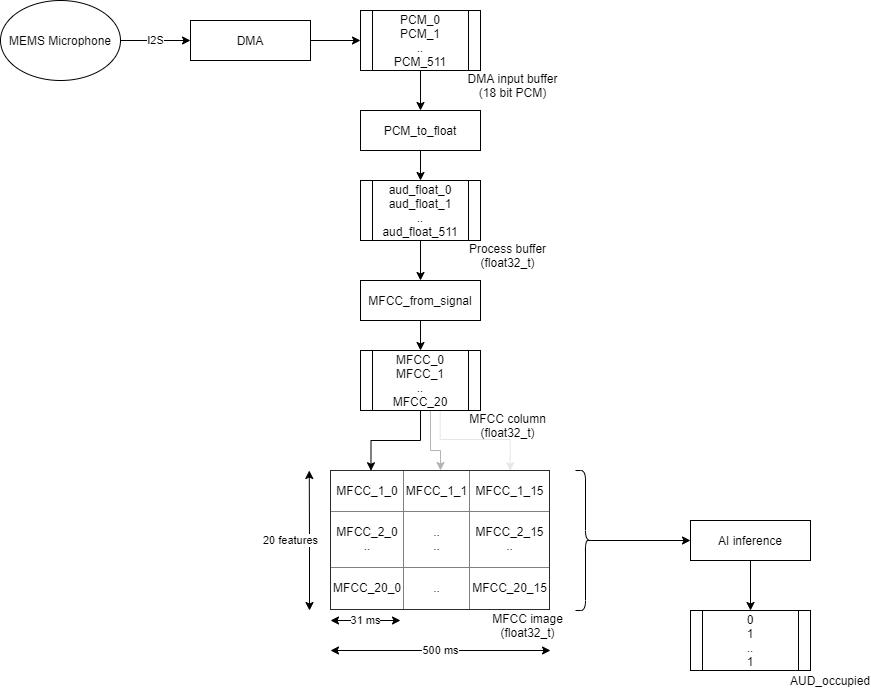
\includegraphics[width=0.9\textwidth]{thesistemplate/fig/embedded_aud_proces.png}
    \caption{Embedded AI preprocessing and inference flowchart, once only one column of the MFCC image is computed. For one AI inference step 16 consecutive columns need to be stored, this indicated with different shades of gray arrows above the MFCC image.}
    \label{fig:embedded_ai_proc}
  \end{center}
\end{figure}


\section{Sensor output fusion with State Machine}

The last step to form a multisensory room occupancy device prototype is to merge the audio-based predictions from the machine learning model and the signals from the PIR motion detection sensor. Since the PIR sensor already provides a digital output when movement is detected, no additional signal processing was applied to the sensor output. After the corresponding pin is configured as digital input on the MCU, each time a rising edge occurs (change in value from 0 to 1), it will trigger a dedicated GPIO interrupt request (EXTI\_IRQ) which is then handled by software callbacks.

An essential question in the design of the fusion algorithm is, whether what is the relative importance of each sensor prediction in various situations and how to form a framework that can incorporate these subtle differences. On an empirical basis, PIR sensors can reliably detect when someone entered the room (high True Positive rate) and have few or no false triggers when the room is empty (high True Negative rate). From a user experience point of view, False-negative predictions are the most visible, unpleasant misbehavior, which needs additional correction. Namely, the situations after one goes into a room, get recognized by the PIR first, but if she stays there seated, the sensor could miss the small movements and falsely predicting an empty room. The introduction of another information source in these states can improve the overall experience by a large amount.
Moreover, preliminary tests with the sound-based classification suggest that microphone or unexpected noises can trigger the model in some situations generating random false positive samples.

Considering the sensor differences a weighted sum of the outputs was constructed, referred to as confidence from now on. The confidence is a value from 0 to 100\%, indicating the confidence in the prediction that one or multiple persons are using the room. If no reinforcement comes from the sensors the value is decreasing linearly. The rate is configurable to imitate more or less aggressive light switching behavior. The default value for the demo is a 5\% decrease every second. The PIR sensor trigger immediately boosts the confidence up to 100\% and one sound-based prediction adds 10\% to the total confidence value.

The designed State machine transition diagram is shown at \autoref{fig:state_mach}. The two states are the Occupied and the Unoccupied room states and the transition between them is based on the current confidence value. As it is visible on the image the two state transition values are 60\% and 40\%, which creates a hysteresis effect, making the transition more reliable from an outside perspective.



\begin{figure}[ht!]
  \begin{center}
    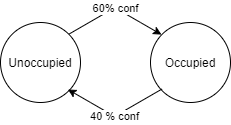
\includegraphics[width=0.4\textwidth]{thesistemplate/images/state_mach.png}
    \caption{State machine transition diagram based on confidence values.}
    \label{fig:state_mach}
  \end{center}
\end{figure}


\begin{figure}[h!]
  \begin{center}
    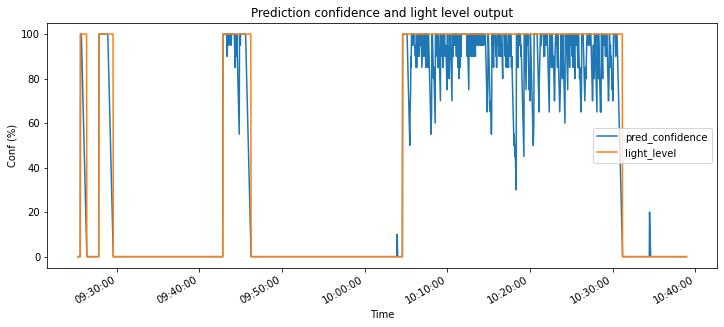
\includegraphics[width=1\textwidth]{thesistemplate/fig/conf_with_lights2.png}
    \caption{Room occupancy confidence with controlled light level values.}
    \label{fig:conf_with_lights}
  \end{center}
\end{figure}

\chapter{Evaluation}
\label{chapter:evaluation}

% \emph{[Deployed model performance evaluation,  Real time prediction tests] }
%  \bigskip

In the following section, the last step of the project development, the testing will be elaborated. Starting from the problem definition, the multisensory solution will be contrasted to the traditional PIR-only light control algorithms in the selected environments. The pilot study involved extensive data collection from all modules to best evaluate and demonstrate the general differences and edge cases in light control behavior.

\section{Test environment}

In the selection of the test environments, the main objective was to identify places where the PIR-based light control solutions notoriously struggle, where there is the most need for alternative approaches. Finding those places and evaluate the effectiveness of the introduction of sound information is key to the viability of the project.

Among company office premises one of the most problematic room types is the private meeting room from an automatic lighting control or presence detection standpoint using traditional PIR sensors. Due to their small size, employees tend to use them for joining a virtual meeting alone or hop in for private phone calls for a short amount of time, so they do not disturb others while having a conversation. Office phone booths have usually one seating place only with limited options for any movement, which makes it hard for PIR sensors to detect motion.

The assembled prototype is then placed in such a private phone booth for testing purposes as it is visible on \autoref{fig:testbox_desk}. From the outside and LED strip indicates the automatic lighting control decisions made by the algorithm based on the audio and PIR measurements discussed earlier. Only the microphone port and the PIR sensor are exposed in the direction of the user, power cords were concealed in the back of the device.


\begin{figure}[t!]
  \begin{center}
    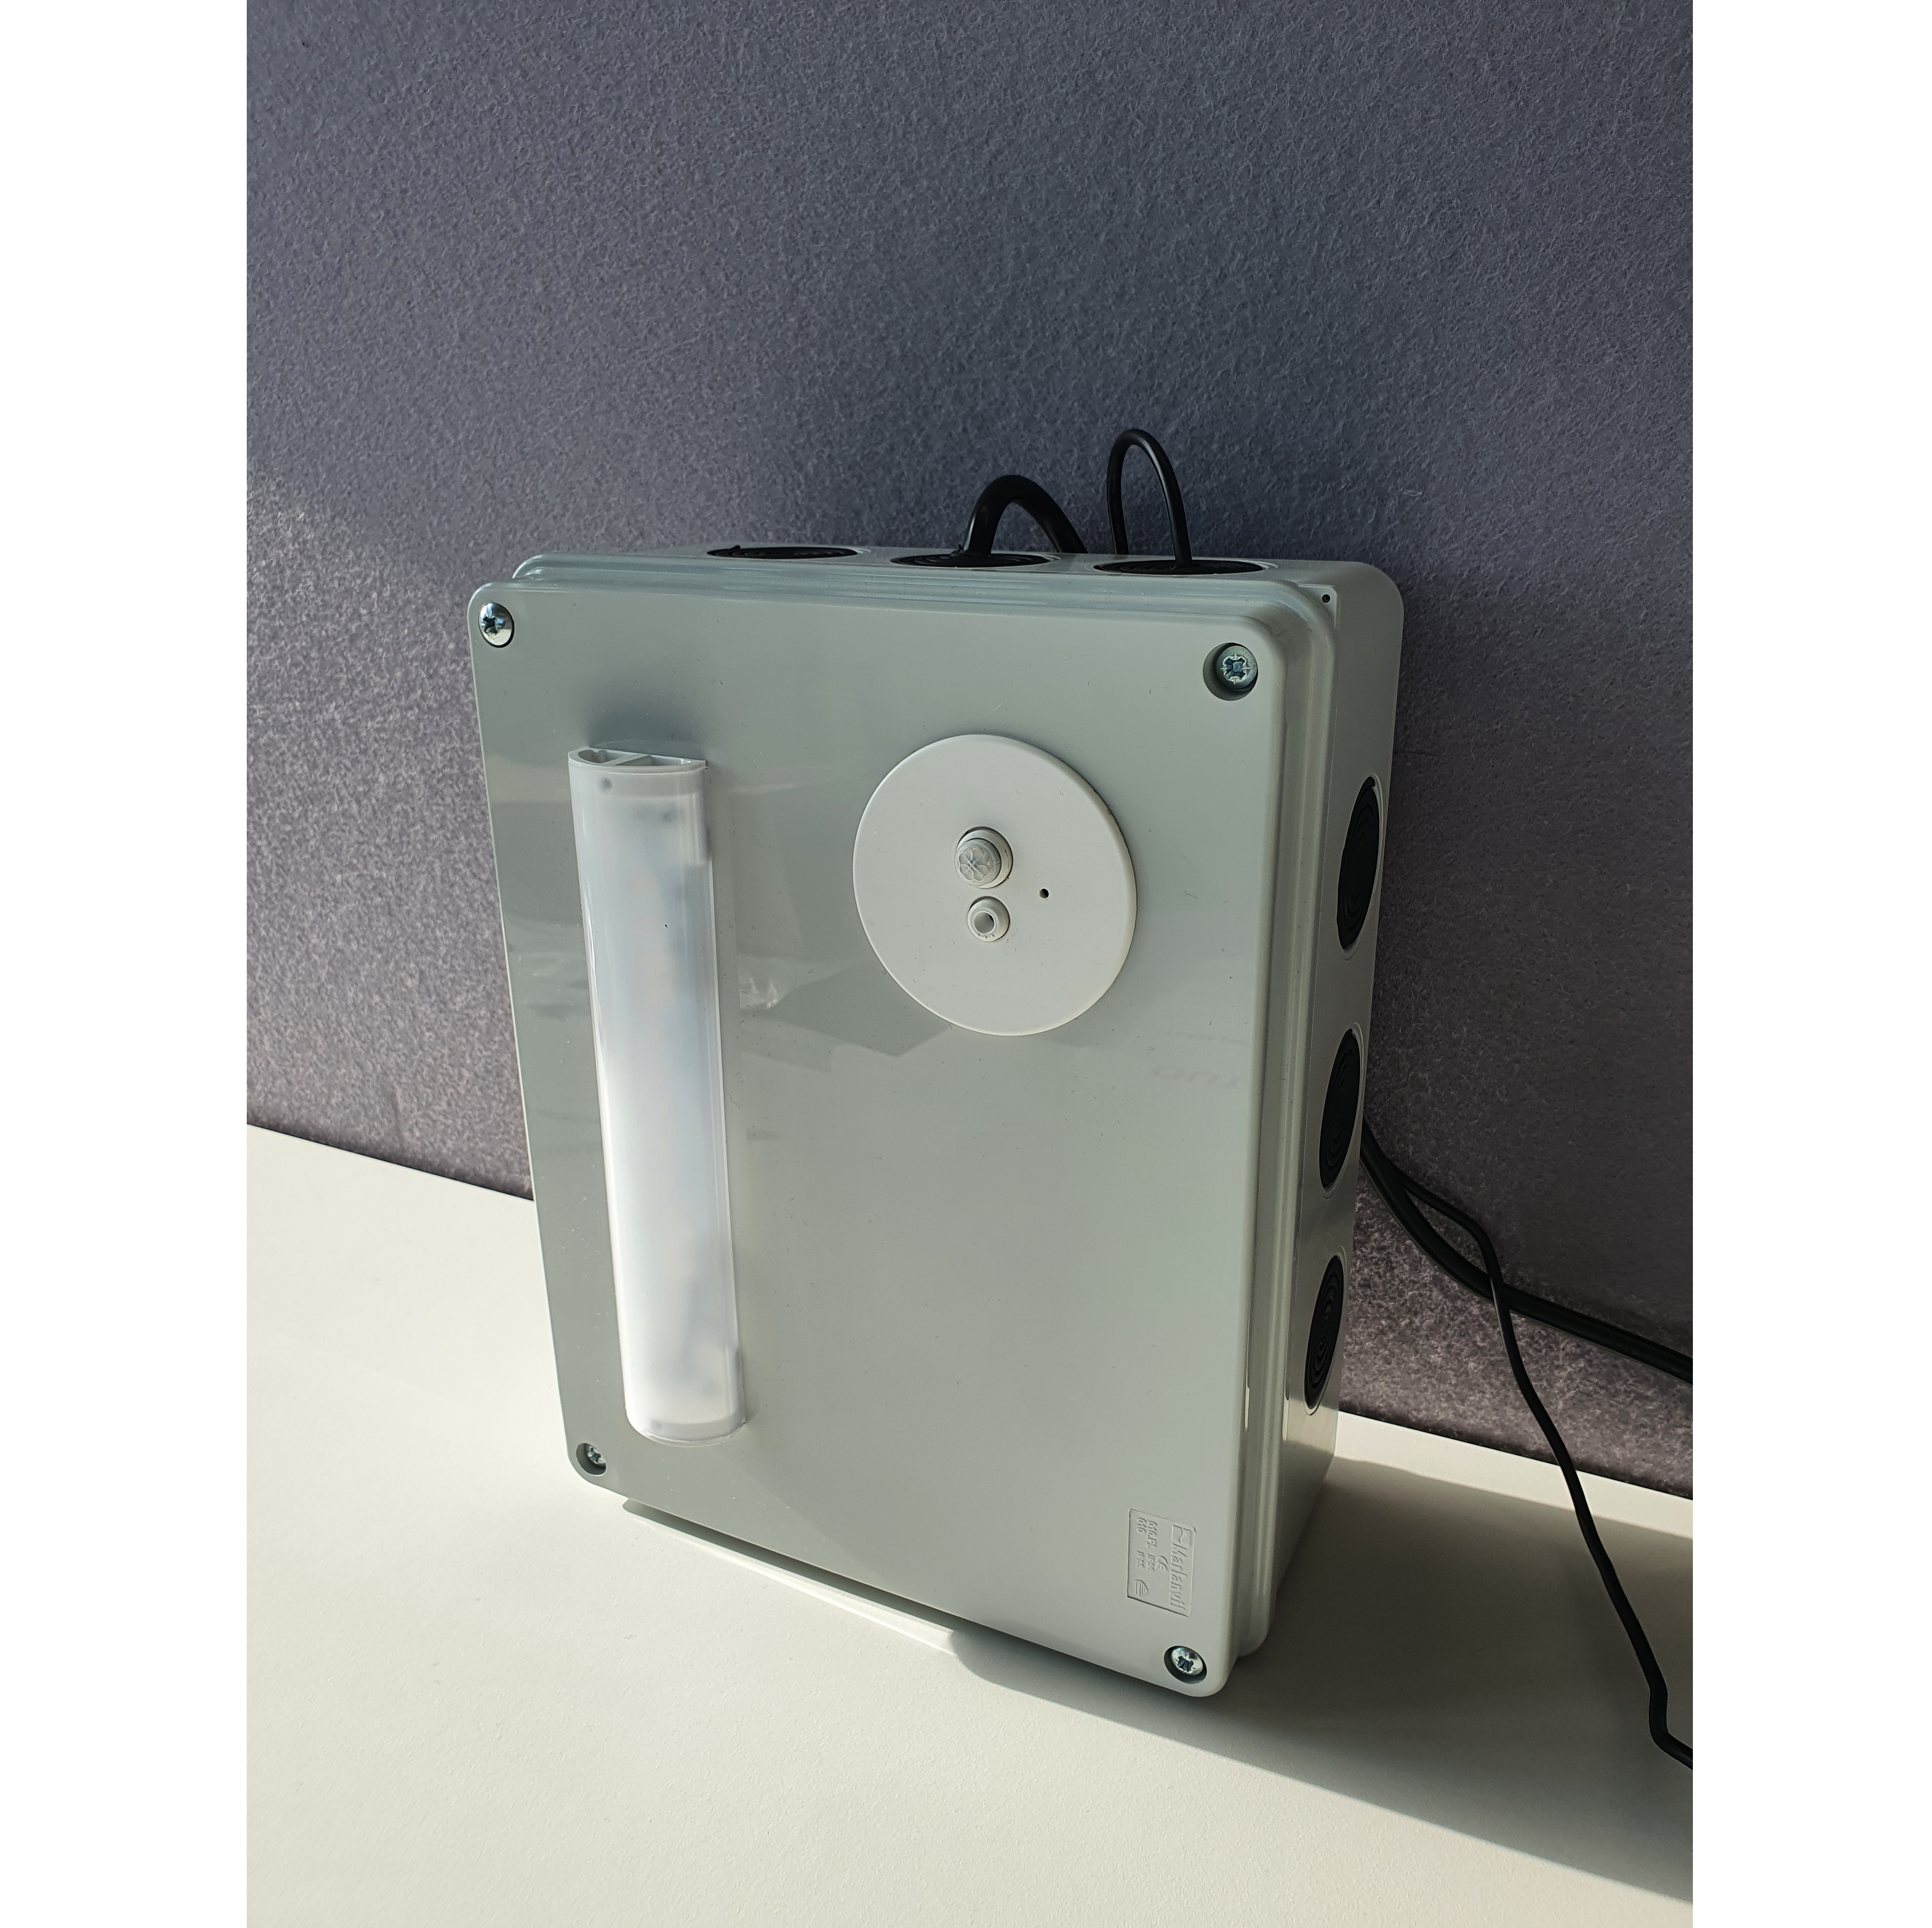
\includegraphics[width=0.5\textwidth]{thesistemplate/images/testbox_11.jpg}
    \caption{The assembled prototype for testing, LED light source attached to the left side while audio and PIR sensors to the top right part of the box.}
    \label{fig:testbox_desk}
  \end{center}
\end{figure}


For logging and data visualization additional hardware extensions and minor software modifications were necessary for the setup, given the limited amount of memory of the microcontroller and relatively difficult interfacing options with remote services. Therefore an additional Raspberry Pi 4B (rPi) was added to the box which logged the prediction confidence values with a timestamp every time it arrived from a preconfigured serial port. The extra hardware is placed to the top right part of the box, as it can be seen on \autoref{fig:testbox_inside}. The microcontroller code is altered to update the rPi each time it changes the confidence value. The rPi then saves the data incrementally to a file and streams it to an open-source cloud data visualizer for real-time status tracking.

For comparing the predictions from the prototype we need to obtain the ground truth for presence in the given meeting room and collect PIR data from the existing lighting control infrastructure. For simplicity, the ground truth was recorded manually by the author, given the fact that due to the low office usage there were only a few usages of meeting rooms per day. The ground truth contains the entry and exit time of a room occupant with one-second precision. Each testing room was equipped with a ceiling-mounted PIR sensor which constantly sends movement detection signals to the private cloud service for space usage monitoring. The actual luminaire light level can be inferred from those signals, given that the system is programmed to keep the lights on until a certain amount of time after each movement trigger. This timeout value can adjust the aggressiveness of the light control strategy and it was fixed to 6.5 minutes in our case as a typical value.


\section{Test results}

An example test sequence result corresponds to a regular working day morning is reported at \autoref{fig:light_output_comp}. As the first plot shows there were four occurrences when the phone booth was occupied for a different length ranging from a few minutes to a half an hour session approximately. Both solutions were able to sense the incoming person instantly but there were significant differences in the detection at the end of the session. PIR-only-based solutions are needed to keep the light on much longer to avoid false off decisions during a meeting due to lack of movement. This misbehavior was caught during the data collection and was indicated with gray area in the second plot. This represents a malfunction in the control process, and which period was correctly classified by the fusion sensor based solution. Most probably the algorithm prediction was reinforced by the sound information in that time interval when there was no movement registered.

\begin{figure}[ht!]
  \begin{center}
    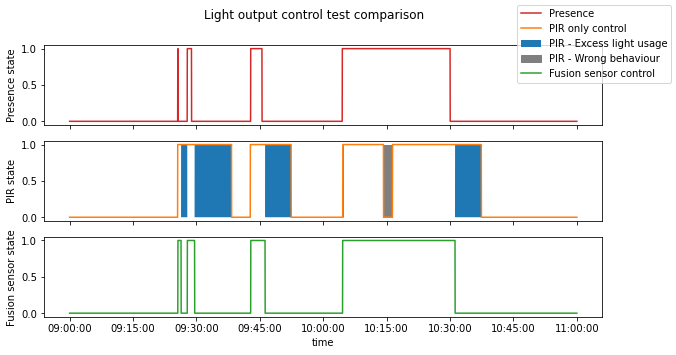
\includegraphics[width=1\textwidth]{thesistemplate/fig/light_output_control_aug23.png}
    \caption{PIR only and Multisensory light level control strategy results compared to ground truth.}
    \label{fig:light_output_comp}
  \end{center}
\end{figure}

The additional sensor allows a more aggressive turn-off policy which reduces excess energy usage in the building. The surplus which is the difference between the PIR only and the Fusion sensor based solution is indicated by the blue area in the second plot. Following the proposed approach approximately 80 \% of the excess energy could be saved by the reduction of timeout values for this particular test case.

\begin{figure}[ht!]
  \begin{center}
    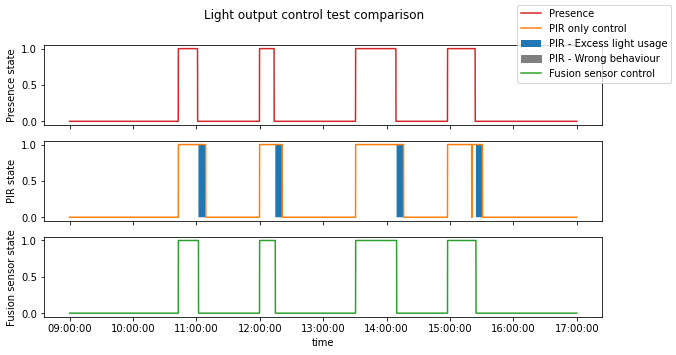
\includegraphics[width=1\textwidth]{thesistemplate/fig/light_output_control_aug27.png}
    \caption{PIR only and Multisensory light level control strategy results compared to ground truth.}
    \label{fig:light_output_comp}
  \end{center}
\end{figure}


\begin{figure}[h!]
  \begin{center}
    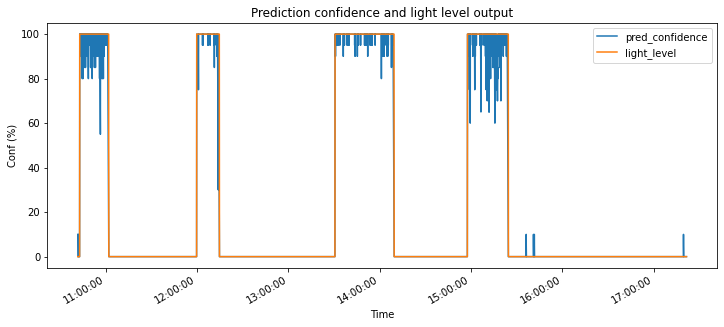
\includegraphics[width=1\textwidth]{thesistemplate/fig/conf_with_lights3.png}
    \caption{Room occupancy confidence with controlled light level values.}
    \label{fig:conf_with_lights}
  \end{center}
\end{figure}


% \begin{figure}[ht]
%     \centering
%     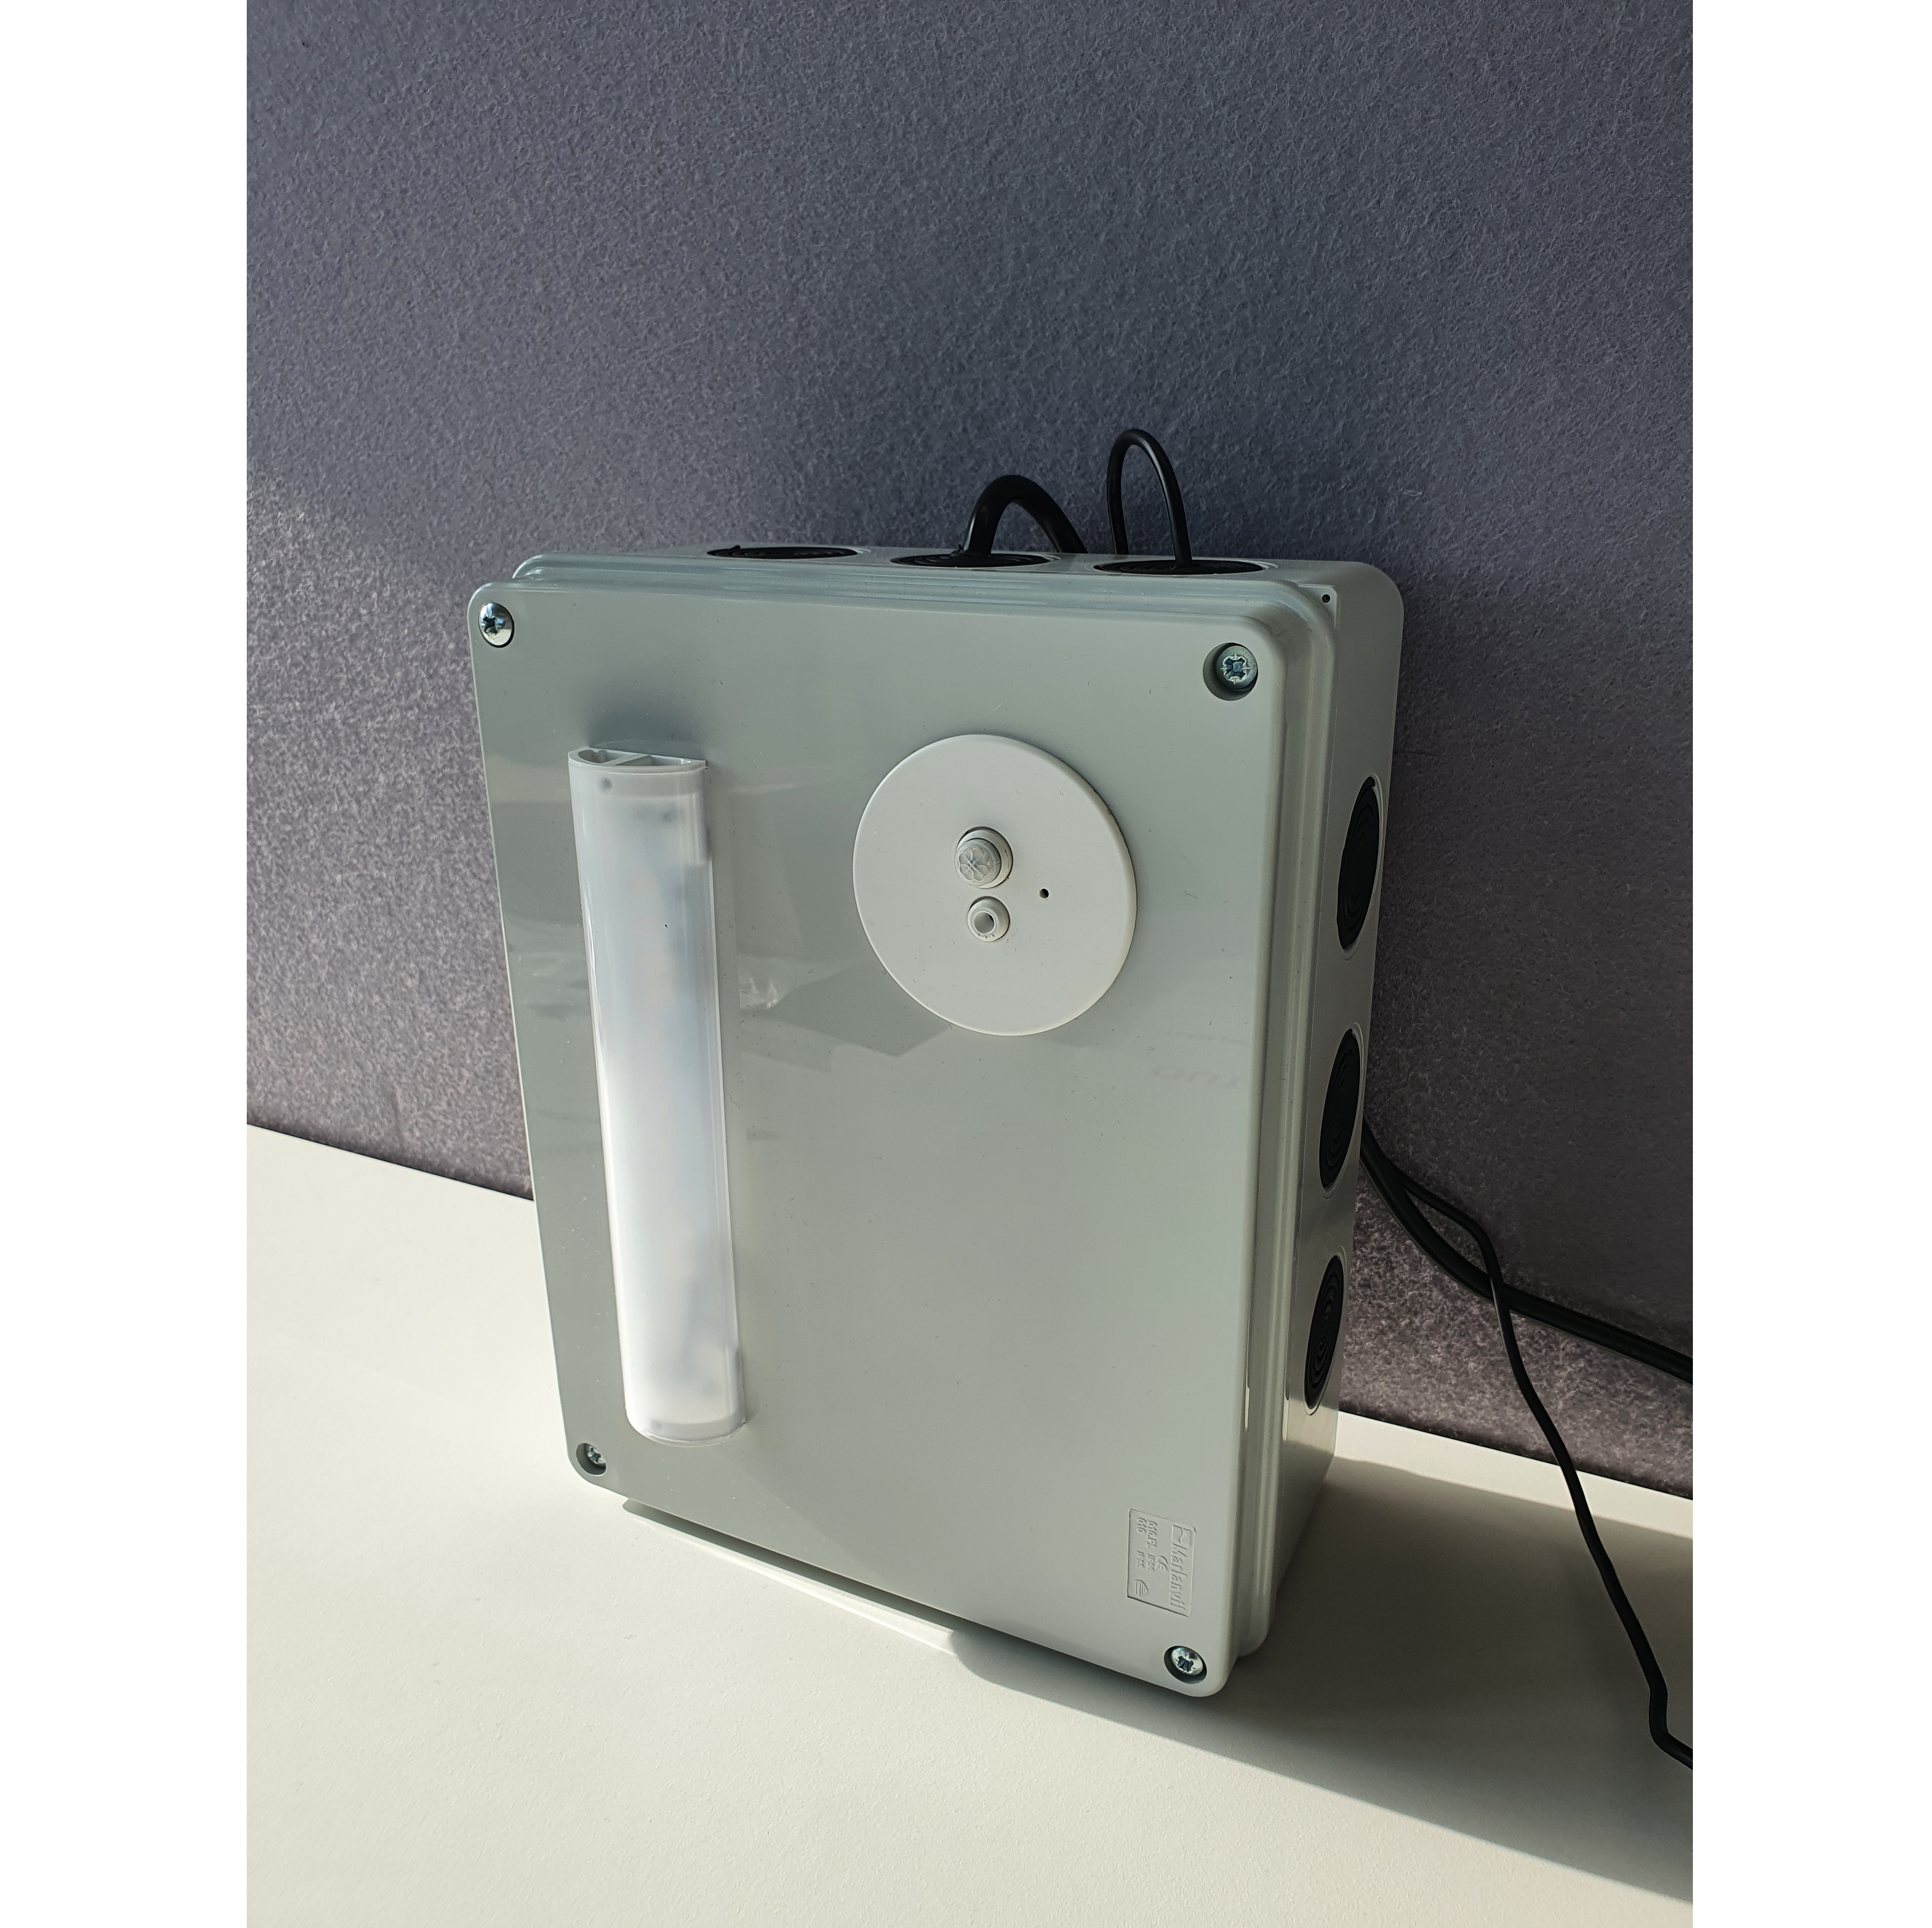
\includegraphics[width=6.5cm]{thesistemplate/images/testbox_11.jpg} 
%     %\hfill
%     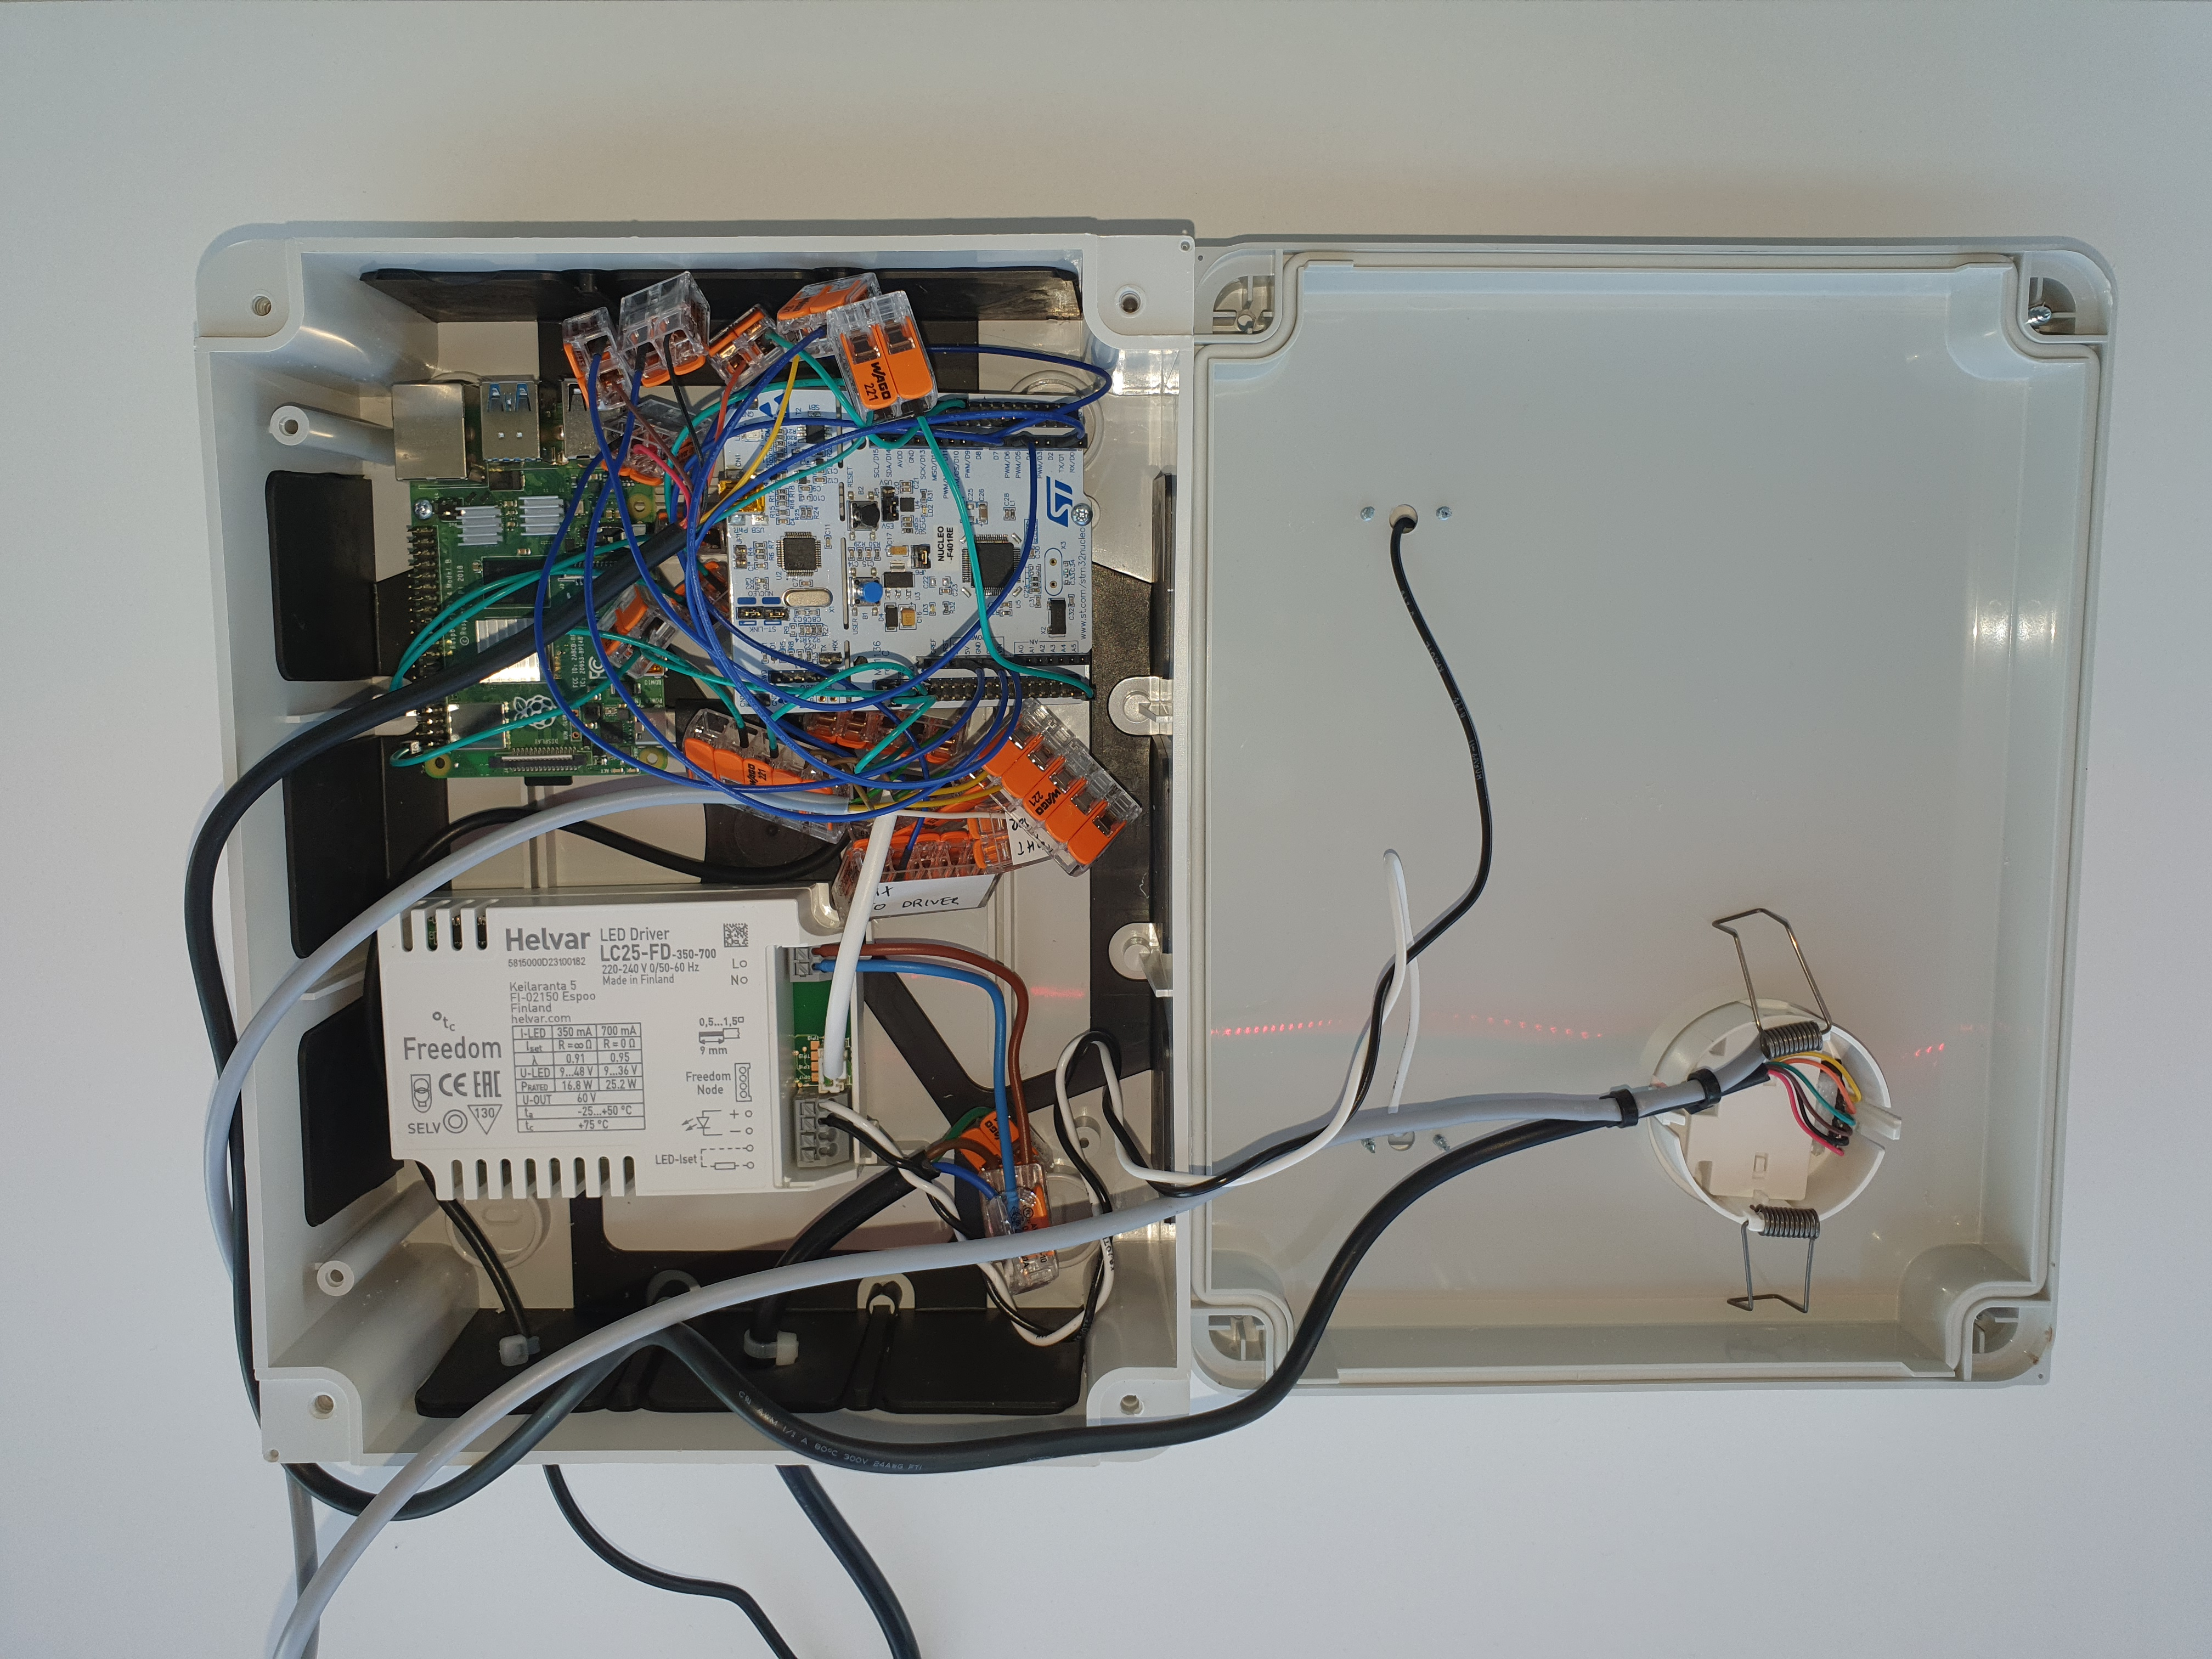
\includegraphics[width=6.5cm]{thesistemplate/images/testbox_2.jpg}
%     \caption{Inside of the prototype for multisensory room occupancy prediction, audio and PIR sensors are connected to the ST development board (white), while a Raspberry Pi 4B (green) is utilized for streaming confidence status. Small LED strip also attached to the outside, controlled by a Helvar LED-driver (white box)}
%     \label{fig:testbox}
% \end{figure}


\begin{figure}[ht!]
  \begin{center}
    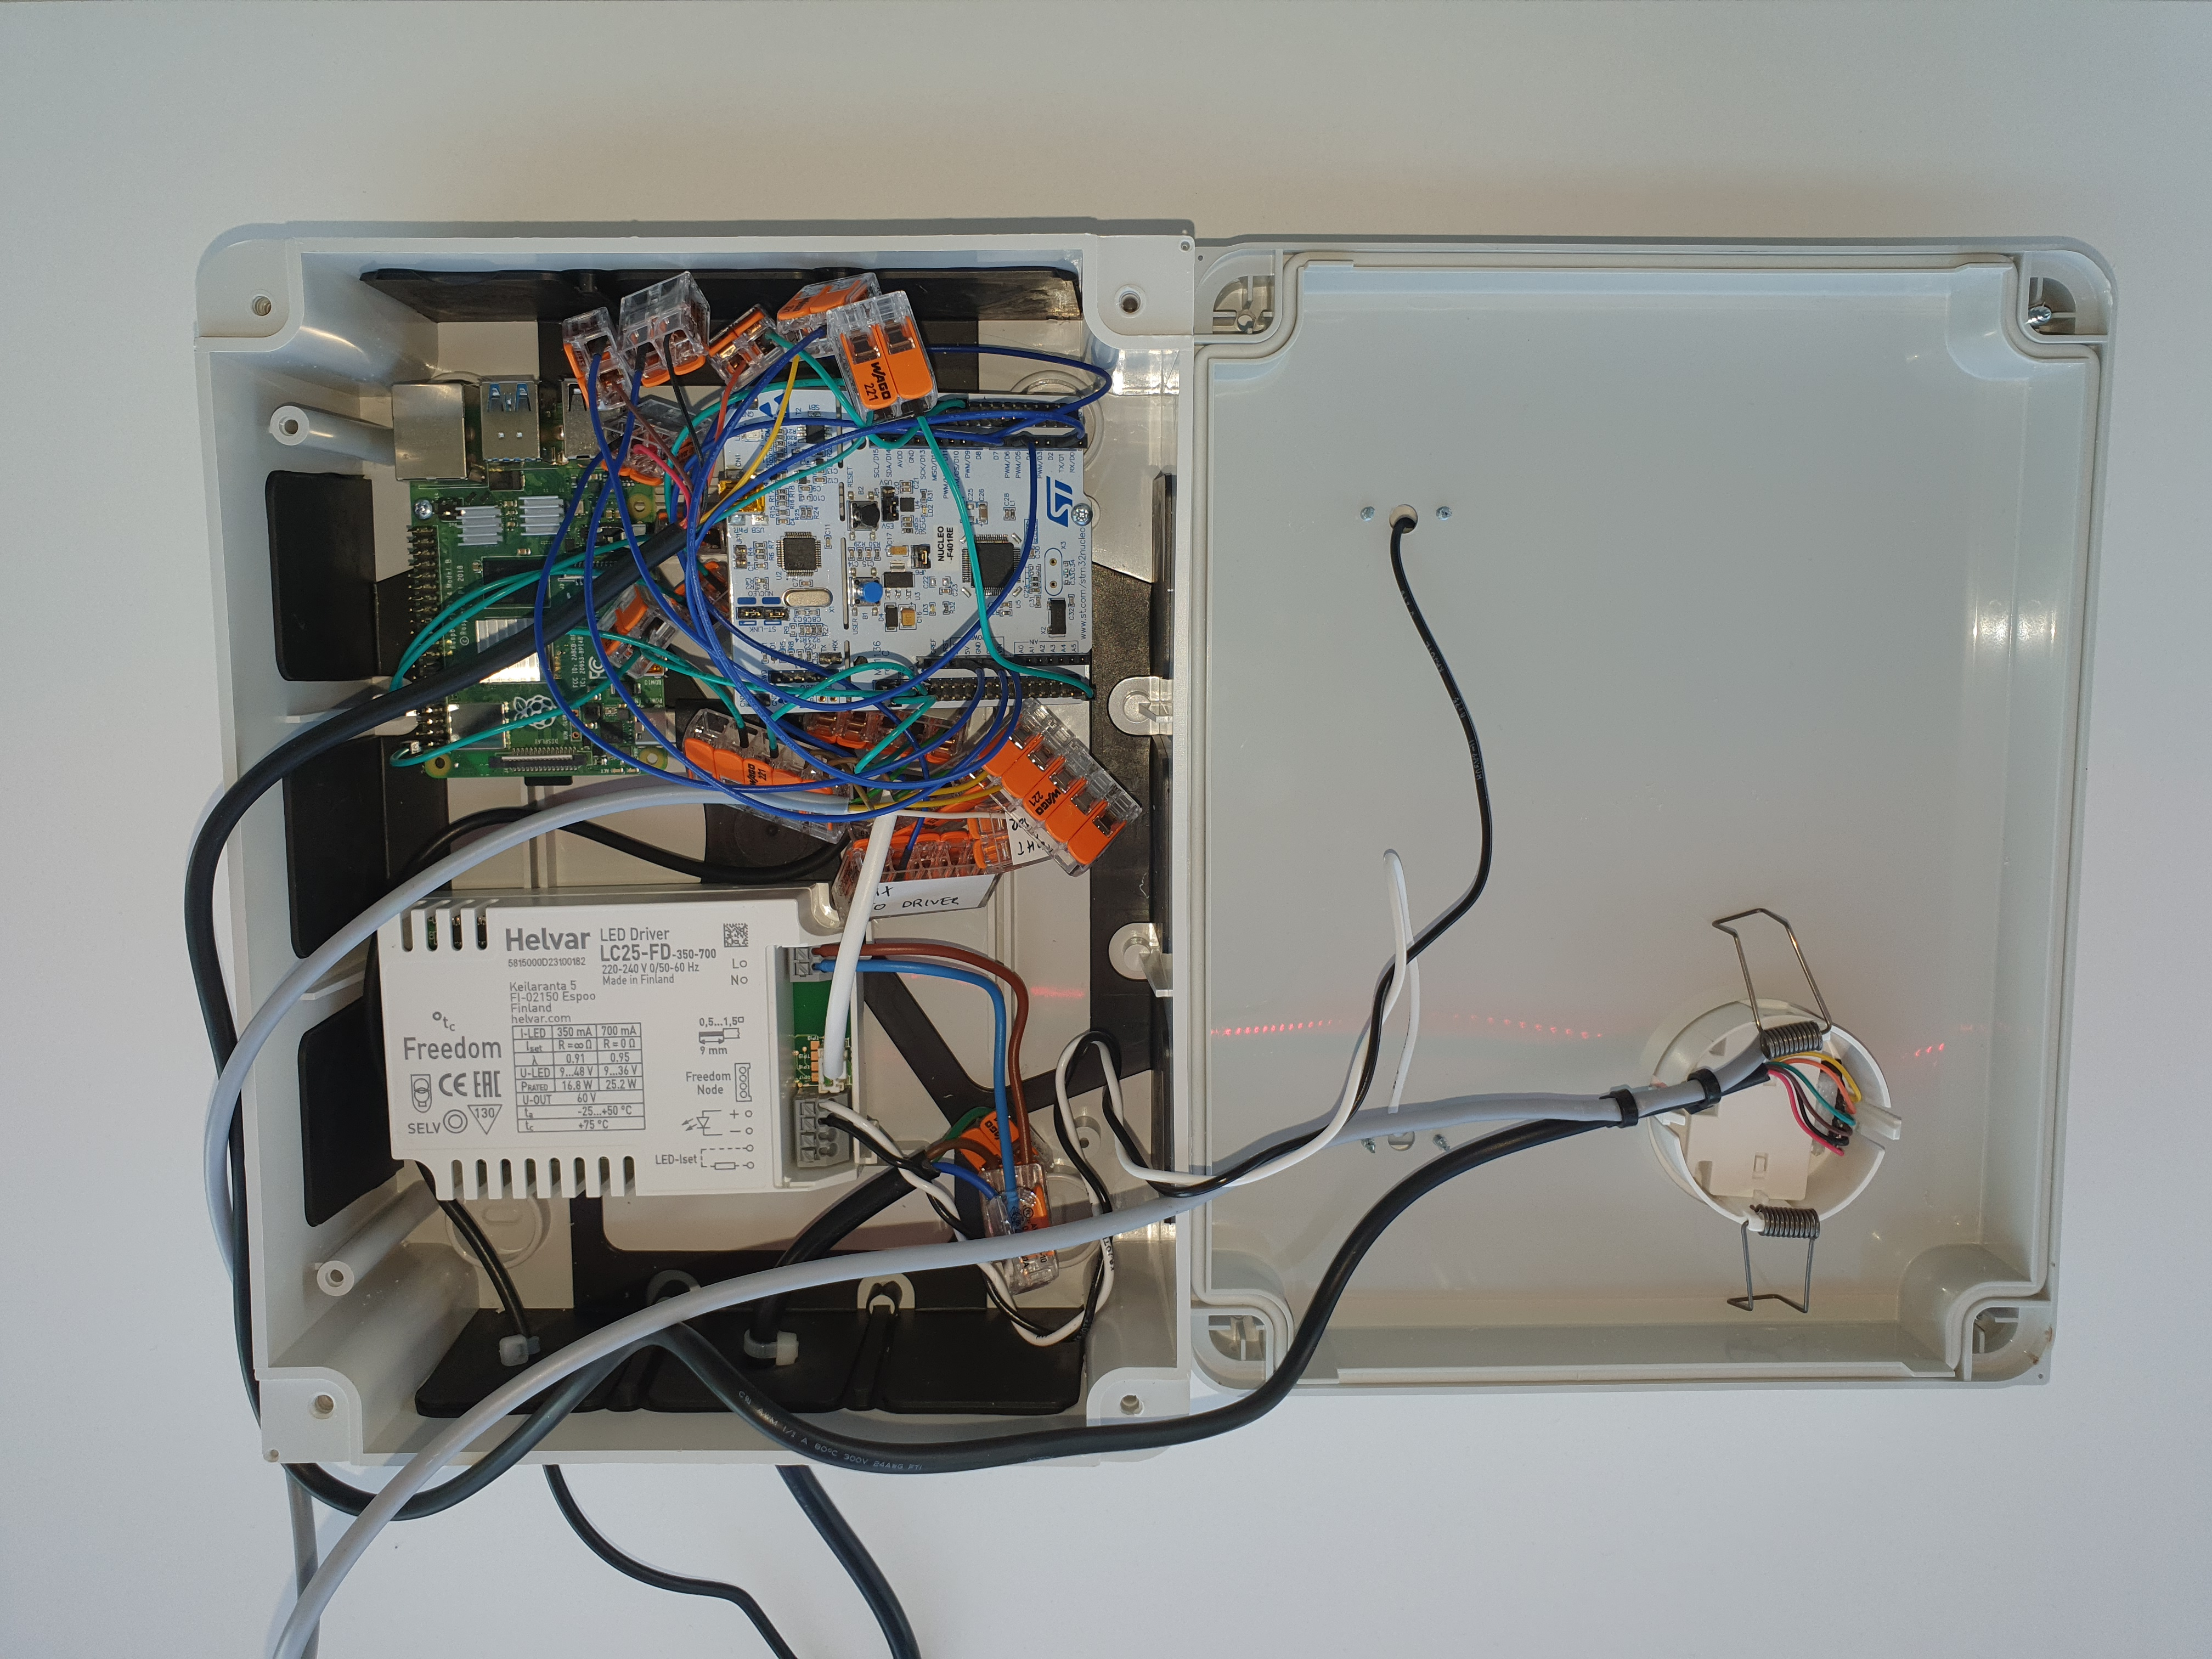
\includegraphics[width=1\textwidth]{thesistemplate/images/testbox_2.jpg}
    \caption{Inside of the prototype for multisensory room occupancy prediction, audio and PIR sensors are connected to the ST development board (white PCB), while a Raspberry Pi 4B (green PCB) is utilized for logging prediction confidence status. Small LED strip also attached to the outside, controlled by a Helvar LED-driver (white box).}
    \label{fig:testbox_inside}
  \end{center}
\end{figure}

% \begin{figure}%
%     \centering
%     \subfloat[\centering label 1]{{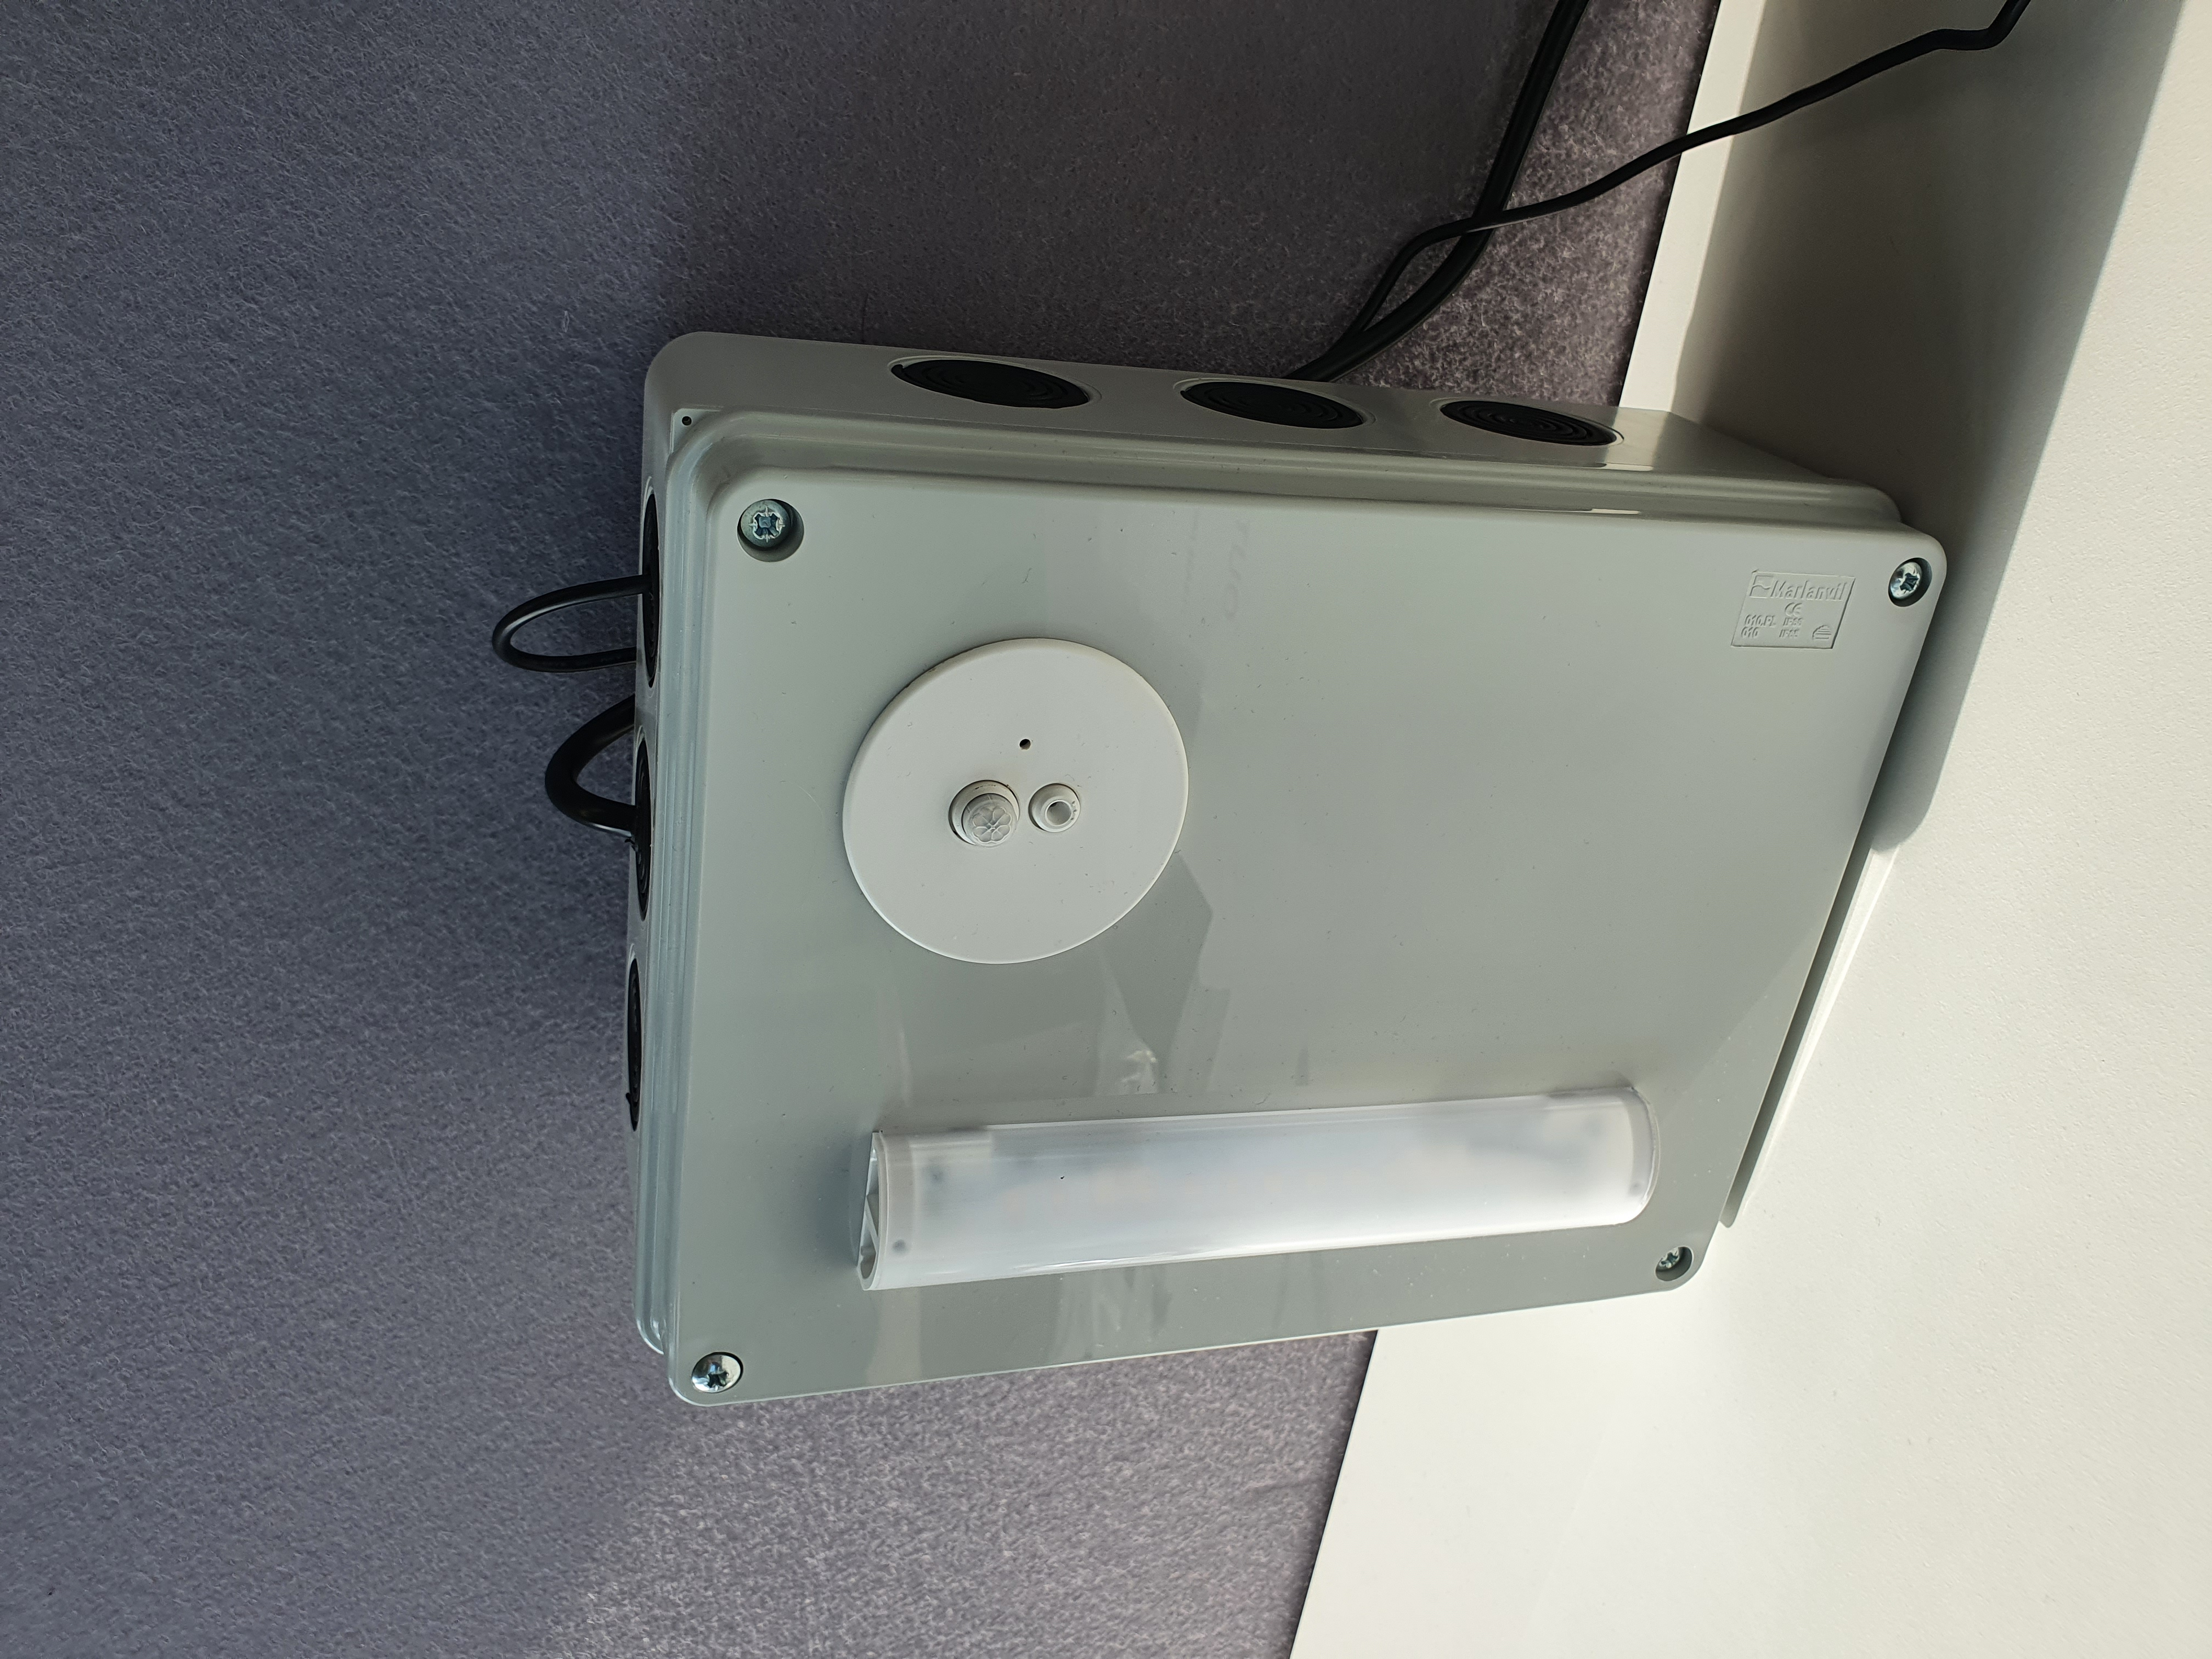
\includegraphics[width=5cm]{thesistemplate/images/testbox_1.jpg} }}%
%     \qquad
%     \subfloat[\centering label 2]{{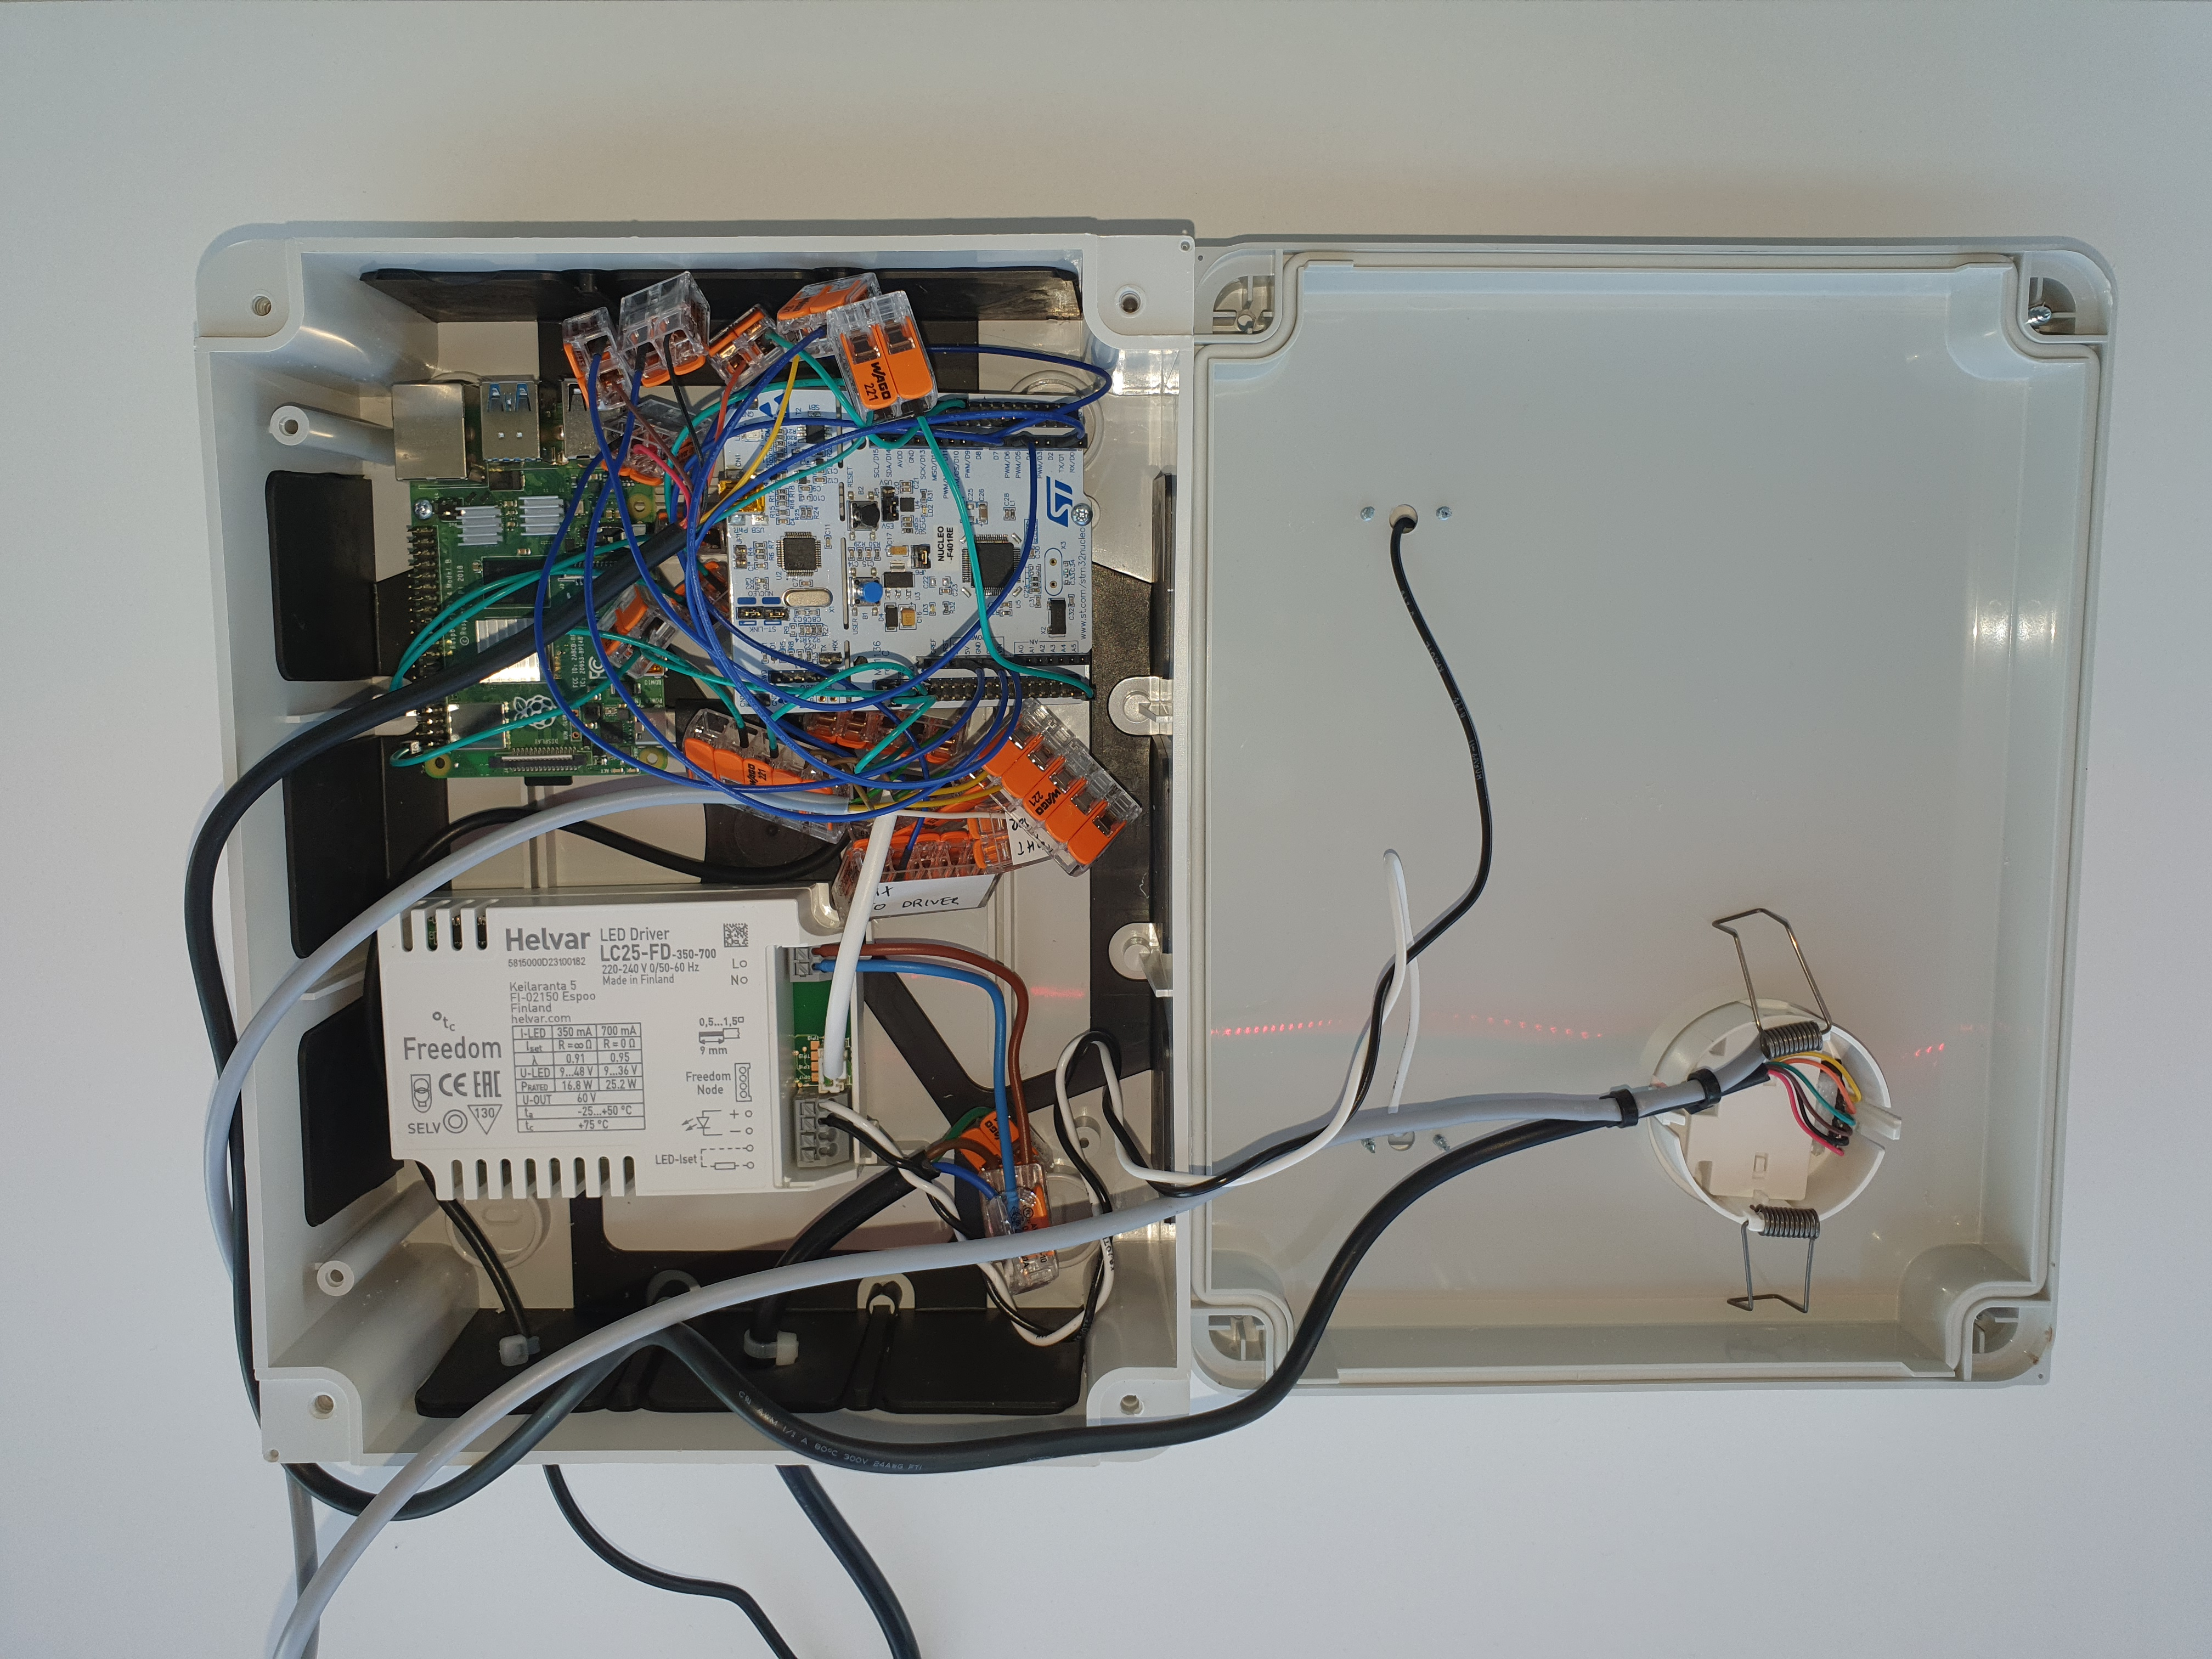
\includegraphics[width=5cm]{thesistemplate/images/testbox_2.jpg} }}%
%     \caption{2 Figures side by side}%
%     \label{fig:example}%
% \end{figure}

\section{Limitations of the used approach}

The multi-day test of the prototype has also revealed some of the weaknesses and hard limitations of the selected sensors and developed algorithms. One such extreme case is shown at \autoref{fig:light_output_faulty}. Unfortunately, the multisensory approach did also suffer from false-negative predictions and turned off the LED strip in situations where the space was occupied by an office worker. As it turned out the person did participate in a virtual meeting during the faulty light control behavior but only listened to others through a headset, leaving a minimal amount of noise or movement for the sensors. Since the current implementation applies less than 30 seconds of timeout this design choice turned to be too aggressive for this particular scenario. However, fine-tuning timeout values and adjusting weights assigned to sensor outputs are outside of the scope of the thesis, since it would require a more thorough analysis of the various use cases.




\begin{figure}[ht!]
  \begin{center}
    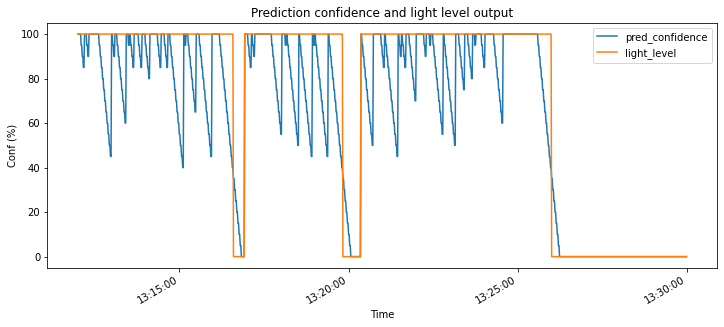
\includegraphics[width=1\textwidth]{thesistemplate/fig/light_output_control_bad.png}
    \caption{Malfunctioning light level control scenario, while room occupancy. The quick jumps back to 100\% are due to PIR triggers, but there is only little reinforcement from sound, which makes the timeout value too short and producing False Negative predictions. }
    \label{fig:light_output_faulty}
  \end{center}
\end{figure}

 
\chapter{Discussion and Future Work}
\label{chapter:discussion}

% Ath this point, you will have some insightful thoughts on your implementation and you may have ideas on what could be done in the future. This chapter may be combined together with the evaluation chapter. All the now insights and findings are given here! This chapter is a good place to discuss your thesis as a whole and to show your professor that you have really understood some non-trivial aspects of the methods you used.


In this thesis, the application of machine learning on an embedded microcontroller was explored in the context of real-time presence detection and lighting automation. Although Convolutional Neural Networks combined with MFCC images have proven to be effective to spot human speech in the audio flow, and combined with PIR, a reliable multisensory device can be created, there are many alternative ways to improve or extend its capabilities.

From an embedded Voice Activity Detector standpoint, further research is encouraged for experimenting with alternative model architectures. Our tests only involved FCN and CNN models, but as software support improves, and more advanced Neural Network building blocks become widely available, there is an expected improvement in model accuracy and performance. The branch of Recurrent Neural Network structures is one of the most promising future candidates for time-series data processing on pre-computed frequency features or the raw audio recording.


Moreover, since the audio signal can be considered as a rich datasource, more complex models and hardware innovations could extract much more information than just the presence of speech. Promising future steps include people counting or crowd size estimation from one microphone source, or sound source localization by the application of a mic array.

As in most Deep Learning applications, the dataset fundamentally determines the model capabilities, the variety and size of the training examples should not be a limiting factor during development. A more thorough analysis of the most common use cases and large-scale field data collection would be advisable for increased robustness. To reduce false-negative predictions during intervals without speech, additional data sources could be considered. Focusing on spotting keyboard typing and mouse clicking in the audio feed could significantly improve the overall lighting control policy, provided quality microphones and relatively low background noise in the selected rooms.  

Furthermore, as previous research suggests, there are great added benefits employing one or multiple analog PIR sensors in the sensor network, as they give more accurate signal related to movement or number of occupants but require additional signal processing and data analysis, which was outside of the scope of the thesis.



% JUHAA
% finding the best model
% - not only speech, but a model especially for keyboard typing

% gray is more important than power saving, short meetings power saving long ones less false negatives
% silence between speech to optimize the timeout value of the algorithm
 
\chapter{Conclusions}
\label{chapter:conclusions}

% Write down the most important findings from your work.
% One to two (never over three) pages might be a good limit

%LAURA
% 9 should repeat the main results/achievements.  (Keep in mind that most people will first look at the abstract, then introduction & conclusions (or only conclusions) and only after that, have a look at the whole thing, if they think it’s worth the time.  )


% TOOM NEW
% The title and the text do not match; the text is a summary of what has been presented, whereas 'conclusions' suggests that this would summarize the outcomes "what was learned". 

The combination of Mel Frequency Cepstral Coefficients and Artificial Neural Networks have been proven effective in many audio-related real-world scenarios, although real-time embedded execution was often limited by the increased computational complexity compared to traditional algorithms. 

In this thesis, we have designed and implemented a prototype of a multisensory presence detection device based on sound and PIR information. The main contributions were the custom-designed machine learning-based algorithms used for audio feature extraction and classification both on desktop and embedded level and the sensor output fusion constructing a final prediction confidence value.

In the development of the audio-based presence detector, the selection of the right feature set played a significant role in the efficient implementation and allowed the usage of smaller machine learning models. The computation of MFCC features is tailor-made for speech recognition purposes and has highly optimized library support for most platforms. Building on top of those features the machine learning model could be reduced to a single classifier structure. Additionally, audio data collected from different sources enhances the reliability of the system and reduces false positive predictions.

In conclusion, as the test results demonstrates, audio-based presence detection has significant research and business potential especially when it is used with other sensors. Moreover, further exploration is encouraged to improve prediction accuracy by more reliable feature extraction or with the introduction of novel sensor inputs.

% First, we have introduced the problem and motivated the need for innovation with the issues the industry is currently facing. This was followed by a short overview of the latest research in audio and PIR-based information processing and its usage in lighting automation.

% Secondly, we have presented a theoretical basis for understanding the used technologies in the audio-based presence detection and implementation sections, namely the working principles of the PIR sensor, MFCC feature extraction, and the most common building blocks of modern Artificial Neural Networks.

%In the Audio-based presence detection chapter, we have constructed a dataset for training using manual recording and external sources and demonstrated high accuracy models found in a grid search. The best-performing models were then selected for embedded implementation where a more thorough analysis of the computational and memory need was presented. The thesis gives a practical suggestion also for the different sensor output fusion by weighting them to strengthen the advantages of each in a State Machine model.

% Finally, in the evaluation section, we have compared our newly proposed solution to the competition and measured the energy saving achieved by the multisensor solution.





% LAURAA


% First of all, I think the thesis is a bit on the long side, which I think you should keep in mind when making changes.  Especially I think that Chapters 1-4 take too much space while 8&9 could be longer

% Especially when it comes to Chapter 1, I’d recommend you think which are the main 3 things you want the reader to remember from that part, and basically remove everything else.  (Actually, you could have the table of contents open and list the main 3 items for each chapter / subchapter, and then check how clearly those items stand out from your text, and if needed, reduce the less important parts so that the important is easier to see).

% In Chapter 2, you should try to fit the intro to the chapter (before 2.1 begins) in one paragraph.  In my opinion, it is not necessary to discuss the contents of subsubchapters (2.1.x) in the opening.  
% Contents of 3.1.1. would perhaps fit better in 2.1 because now you discuss PIR problems before telling much about what PIR is and how it works.  

% The other thing is that the level of knowledge you assume from  the reader seems to vary.   You could have in mind some high-school friend maybe, who went to study something technical but not really computing/automation.  They should be able to follow your thesis.  Do they know what PIR is?  What do they know already of machine learning?  (Would they understand your explanation of these things?)

% Then, I recommend spellchecking and grammar checking.  You seem to be leaving out quite often the main verb of the sentence (is, are, were, …) 


% Overall, I would say the thesis looks good, but I think a more to-the-point opening would give a better first impression.



% Load the bibliographic references
% ------------------------------------------------------------------
% You can use several .bib files:
% \bibliography{thesis_sources,ietf_sources}
\bibliography{sources}


% Appendices go here
% ------------------------------------------------------------------
% If you do not have appendices, comment out the following lines
%\appendix
%\chapter{First appendix}
\label{chapter:first-appendix}

This is the first appendix. You could put some test images or verbose data in an
appendix, if there is too much data to fit in the actual text nicely.

For now, the Aalto logo variants are shown in Figure~\ref{fig:aaltologo}.

\begin{figure}
\begin{center}
\subfigure[In English]{
\includegraphics[width=.8\textwidth]{images/aalto-logo-en}}
\subfigure[Suomeksi]{
\includegraphics[width=.8\textwidth]{images/aalto-logo-fi}}
\subfigure[På svenska]{\includegraphics[width=.8\textwidth]{images/aalto-logo-se}}
\caption{Aalto logo variants}
\label{fig:aaltologo}
\end{center}
\end{figure}


% End of document!
% ------------------------------------------------------------------
% The LastPage package automatically places a label on the last page.
% That works better than placing a label here manually, because the
% label might not go to the actual last page, if LaTeX needs to place
% floats (that is, figures, tables, and such) to the end of the 
% document.
\end{document}
